\documentclass{aalesson}		% Classe spéciale créée pour les cours d'A. Achim

\usepackage{textcomp}			% jeux de symboles spéciaux
\usepackage{subfig}				% gestion des figures multiples
\usepackage{numprint}			% pour écrire les nombres proprement
\usepackage{sistyle}			% jeux de macros pour les unités SI
\usepackage{multirow,multicol}	% pour des tableaux avancées
\usepackage{rotating}			% rotation
\usepackage{enumitem}			% liste à puce avancées
\usepackage{tikz-qtree} 		% package pour dessiner des arbres en LaTeX
\usetikzlibrary{trees}

\title{GBO-4000 / GBO-7000 \\ Anatomie et structure du bois}
\author{Alexis Achim \\ Alain Cloutier}
\date{Automne 2022}
\info{Notes de cours}
\logo{img/Ulaval}

\newcommand{\flip}[1]{\rotatebox{90}{#1}}

\begin{document}

\maketitle

\dominitoc
\faketableofcontents

\chapter*{Avant-propos}

La mise en page de ce document est calquée sur le modèle de la revue scientifique \href{https://peerj.com/}{PeerJ}. Je tiens à remercier sincèrement Pete Binfield, le co-fondateur de la revue, de nous avoir donné la permission d'utiliser son modèle. J'encourage les étudiants à visiter le site de la revue. Tous les articles scientifiques qu'elle contient sont en libre accès (gratuit pour les lecteurs).\\

Le contenu des notes de cours a évolué à partir d'un document de départ rédigé par Alain Cloutier. Depuis 2007, Alexis Achim et Alain Cloutier sont co-responsables du cours et ils ont travaillé ensemble à la mise à jour de certaines parties. La partie dur la physiologie de l'arbre du chapitre 2 est issue des notes de cours de David Pothier. Nous tenons à le remercier d'avoir partagé ses notes avec nous.\\

Plusieurs des illustrations ont été développées par Julie Ferland. Nous souhaitons aussi à souligner la contribution extraordinaire de Jean-Romain Roussel qui a réalisé la migration entre les formats MSWord et \LaTeX en plus de travailler à la production de certaines des illustrations. Si le format des notes de cours peut faciliter votre apprentissage, c'est grâce à lui.\\

Toutes les images et le texte de ce document sont placés sous licence \href{https://creativecommons.org/licenses/by-nc-sa/4.0/}{Creative Commons CC BY-NC-SA 4.0}
, ce qui implique que vous pouvez les réutiliser, modifier et partager dans un but non commercial et sous la même licence, et sous réserve de citer les auteurs originaux.\\

La citation de cet ouvrage devrait apparaître ainsi: Achim, A., Cloutier, A. 2018, GBO-4000 / GBO-7000 Anatomie et structure du bois -- Notes de cours, Automne 2018, Université Laval, 104 p.\\

 
 Bonne lecture et bonne session.\\
 
 \begin{flushright}
 	Alain Cloutier et Alexis Achim, professeurs
 \end{flushright}

\begin{figure}[ht]
	\centering
	\includegraphics[height=2cm]{img/CC_licence}
\end{figure}


\chapter{Notions générales}

\begin{abstract}
Ce chapitre vous présente certaines notions générales sur le matériau bois. Vous devez retenir les directions et plans principaux dans le bois qui nous serviront dans chacun des chapitres suivants.
\end{abstract}

\minitoc

\section{Introduction}

Le bois est un matériau utilisé par l'homme depuis fort longtemps mais il est encore relativement mal connu sur un certain nombre d'aspects et en particulier au niveau de l'effet des conditions de croissance sur ses propriétés physiques, chimiques et mécaniques et sur son comportement mécanique à long terme dans des conditions hygrothermiques variables. Malgré le développement de nouveaux matériaux, la consommation mondiale de bois va en augmentant au fil des ans (croissance d'environ 1\% par an), au fur et à mesure que la population du globe augmente.\\

Les produits du bois ont plusieurs avantages par rapport à d'autres matériaux \cite{bowyer2007forest}: La ressource est renouvelable dans la mesure où les pratiques forestières sont adéquates. Il est possible d'utiliser une partie de la matière récoltée pour produire l'énergie requise à la fabrication des produits du bois (production de vapeur à partir de chaudières à résidus de bois et d'écorce). Le bois peut être transformé facilement: Il peut être scié pour en fabriquer du bois de construction, tranché pour en faire des copeaux ou des placages, ou réduit en fines particules ou en fibres pour en fabriquer des panneaux composites, du papier ou d'autres produits du bioraffinage. Les forêts peuvent aussi être utilisées à d'autres usages que la seule production de matière ligneuse. Le bois est un matériau naturel dont l'utilisation a relativement peu d'impact sur l'environnement comparativement à d'autres matériaux tels que le béton et l'acier.\\

Nous sommes présentement à un tournant au niveau de l'utilisation du bois. Les forêts vierges sont de plus en plus rares, les bois disponibles sont de plus en plus issus de forêts de seconde venue, souvent de dimension et de qualité inférieures aux approvisionnements antérieurs, ce qui implique des changements de technologie majeurs. De plus, les produits forestiers sont maintenant en compétition avec des produits de remplacement (plastiques, acier, béton, etc.). Cette situation favorise le développement de produits composites à base de bois tels que panneaux, poutres composites, revêtements de planchers et autres. Ces produits ont généralement des propriétés supérieures et moins variables que le bois massif et sont moins contraignants quant à la qualité de la matière première.\\

Le volume de bois sur pied à l'échelle mondiale est présenté au Tableau~\ref{volume}. On remarque les forts volumes présents en Amérique du Sud et en Russie. On remarque aussi que le bois résineux est surtout disponible en Amérique du Nord et Russie, le volume étant deux fois plus grand en Russie. Le volume présent dans une région du monde donnée est important mais la productivité forestière l'est également lorsqu'on parle d'utilisation de forêt de seconde venue. Le Tableau~\ref{accroissement} présente la productivité forestière par région productrice de bois. On remarque un groupe de pays dont les productivités forestières dépassent les 15 m\up{3}/ha année. Ces productivités très fortes sont le résultat de climats favorables mais aussi d'une sylviculture intensive. En comparaison, la productivité forestière du Québec est d'environ 1,0 à 2,0 m\up{3}/ha année.

\begin{table}[ht]
\centering
	
	\begin{tabular}{l c c c}
	\hline
	\bf Région & \bf Résineux & \bf Feuillus & \bf Total \\
	\hline
	\hline
	Amérique du Nord & 31.0 & 15.4 & 46.7\\
	Amérique centrale & 1.9 & 3.6 & 5.5\\
	Amérique du Sud & 0.9 & 90.6 & 91.5 \\
	Afrique & 0.2 & 24.8 & 25.0 \\
	Europe & 8.0 & 4.0 & 12.0 \\
	Russie & 65.3 & 20.6 & 85.9 \\
	Asie & 6.0 & 32.0 & 38.0\\
	Océanie	& 0.7 & 5.3 & 6.0 \\
	\hline
	Monde & 114.3 & 196.3 & 310.6 \\	
	\hline
	\end{tabular}

\caption{\label{volume} Volume ($\times10^9$ m\up{3}) mondial de bois sur pied (d'après \cite{MRN1996}).}
\end{table}


\begin{table}[ht]
\centering
	
	\begin{tabular}{l c}
	\hline
	\bf Région	& \bf Accroissement annuel moyen \\
	\hline
	\hline
	Russie &  2.0\\
	Colombie-Britannique (Intérieur)  & 2.5 \\
	Colombie-Britannique (Côte)  & 5.0 \\
	Scandinavie &  5.0 \\
	États-Unis (Sud) &  6.5\\
	États-Unis (Pacifique – Nord-Ouest) &  7.0 \\
	Australie &  15.0 \\
	Afrique du Sud &  17.0 \\
	Brésil (résineux) & 20.0 \\
	Nouvelle-Zélande &  21.0 \\
	Chili &  22.0 \\
	Brésil (feuillus) & 25.0 \\
	\hline
	\end{tabular}

\caption{\label{accroissement} Productivité (m\up{3}.ha\up{-1}.an\up{-1}) forestière dans diverses régions du monde (d'après \cite{MRN1996}).}
\end{table}

Le bois est produit dans une grande variété de plantes mais nous nous intéresserons au bois produit dans les arbres, c'est-à-dire des plantes ligneuses de plus de 7 m de hauteur caractérisées par un tronc unique plutôt que plusieurs petites tiges. Les plantes ligneuses plus petites sont généralement appelées arbustes. Les arbres sont généralement divisés en conifères et feuillus qui sont très différents au niveau botanique. La Figure~\ref{regneveg} illustre la systématique des plantes appliquée au cas des arbres. Les conifères et les feuillus font partie de la division des spermatophytes (les autres divisions sont les thallophytes (algues et champignons), les bryophytes (mousses et lichens) et les ptéridophytes (fougères, joncs)), ce qui implique qu'ils se reproduisent par graines. Ils sont toutefois dans deux sous-divisions différentes, les conifères étant inclus dans les gymnospermes et les feuillus dans les angiospermes. Les gymnospermes produisent des graines nues et les angiospermes des graines incluses dans un ovaire. Pour fins d'identification, on fait généralement référence au genre et à l'espèce auxquels appartient un arbre. Les noms latins évitent toute confusion avec les noms communs des arbres qui peuvent varier entre les régions. Par convention, on attribue une lettre majuscule au genre et une lettre minuscule à l'espèce (à moins qu'elle ne fasse référence à un nom propre).\\

\begin{figure}[h]
	\centering
	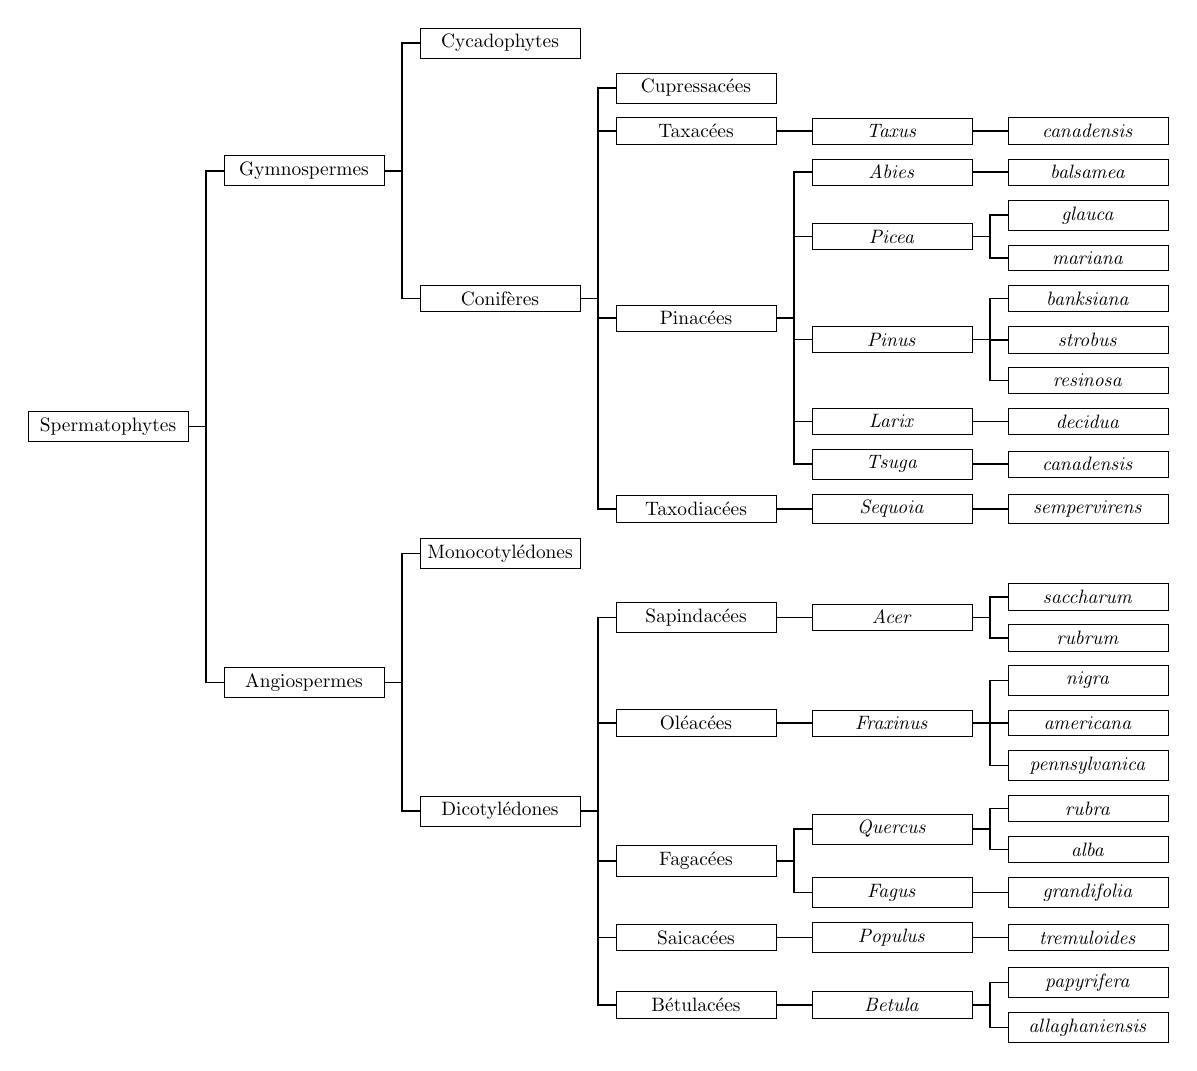
\begin{tikzpicture}[level distance=1.40in,sibling distance=.1in,scale=.7]
	\tikzset{edge from parent/.style= 
			{thick, draw,
					edge from parent fork right},every tree node/.style={draw,minimum width=1in,text width=1.05in, align=center},grow'=right}
	\Tree 
	[. {Spermatophytes}
		[.{Gymnospermes}
			[.{Cycadophytes} ]
			[.{Conifères}
				[.{Cupressacées} ]
				[.{Taxacées} 
					[.{\textit{Taxus}}
						[.{\textit{canadensis}} ]					
					]
				]
				[.{Pinacées}
					[.{\textit{Abies}}
						[.{\textit{balsamea}} ]
					]
					[.{\textit{Picea}}
						[.{\textit{glauca}} ]
						[.{\textit{mariana}} ]
					]
					[.{\textit{Pinus}}
						[.{\textit{banksiana}} ]
						[.{\textit{strobus}} ]
						[.{\textit{resinosa}} ]
					]
					[.{\textit{Larix}}
						[.{\textit{decidua}} ]
					]
					[.{\textit{Tsuga}}
						[.{\textit{canadensis}} ]
					]
				]	
				[.{Taxodiacées}
					[.{\textit{Sequoia}}
						[.{\textit{sempervirens}} ]						
					]
				]
			]
		]
		[.{Angiospermes}
			[.{Monocotylédones} ]
			[.{Dicotylédones}
				[.{Sapindacées} 
					[.{\textit{Acer}}
						[.{\textit{saccharum}} ]
						[.{\textit{rubrum}} ]					
					]
				]
				[.{Oléacées} 
					[.{\textit{Fraxinus}}
						[.{\textit{nigra}} ]
						[.{\textit{americana}} ]
						[.{\textit{pennsylvanica}} ]					
					]
				]			
				[.{Fagacées} 
					[.{\textit{Quercus}}
						[.{\textit{rubra}} ]
						[.{\textit{alba}} ]					
					]
					[.{\textit{Fagus}}
						[.{\textit{grandifolia}} ]					
					]
				]
				[.{Saicacées} 
					[.{\textit{Populus}}
						[.{\textit{tremuloides}} ]				
					]
				]
				[.{Bétulacées} 
					[.{\textit{Betula}}
						[.{\textit{papyrifera}} ]
						[.{\textit{allaghaniensis}} ]					
					]
				]				
			]
		]
	]
	\end{tikzpicture}
	\caption{\label{regneveg} Les arbres dans le règne végétal. Dans l'ordre de gauche à droite: division, sous-division, classe, famille, genre, espèce. Vous apprendrez dans le cadre de ce cours à distinguer chacun des genres présentés à l'aide des caractéristiques anatomiques du bois. On vous initiera aussi à l'identification des arbres sur pied}	
\end{figure}

\todo{Cherchez les noms communs de chacune des espèces représentées dans ce diagramme.}

\section{Principales caractéristiques du bois}

\subsubsection{Les produits forestiers font partie de notre vie de tous les jours}

\begin{itemize}
\item Bois massif
\item Contreplaqué
\item Composites à base de bois
\item Le bois est un matériau composite par excellence
\end{itemize}

\subsubsection{Le bois a une structure cellulaire}

\begin{itemize}
\item Les lumens des principales cellules du bois forment des conduites cylindriques
\item La paroi cellulaire est largement composée de cellulose
\item Les cellules du bois sont liées entre elles par un adhésif naturel: la lignine
\end{itemize}

\subsubsection{Le bois est un matériau orthotrope}

\begin{itemize}
\item Le bois possède une structure orientée selon trois \hyperref[directions]{directions principales} : longitudinale, radiale et tangentielle. Ces trois directions principales forment un système de référence orthogonal. 
\item Les propriétés mécaniques, physiques, thermiques et hydriques varient selon la direction principale considérée. 
\end{itemize}

\subsubsection{Le bois est un matériau hygroscopique}

\begin{itemize}
\item Le bois adsorbe ou désorbe de l'eau en fonction de la température et de l'humidité relative de l'air
\item La température et l'humidité relative de l'air déterminent la teneur en humidité d'équilibre (Héquil) du bois.
\item Une variation de teneur en humidité du bois sous le point de saturation des fibres (psf) implique des changements de dimension : retrait ou gonflement.
\end{itemize}

\subsubsection{Le bois est un matériau hétérogène et variable}

Le bois est un matériau « biologique » donc variable par définition :

\begin{itemize}
\item Présence de nœuds
\item Bois de duramen et bois d'aubier
\item Les conditions de croissance affectent la croissance annuelle et d'autres caractéristiques du bois : masse volumique, longueur des fibres, etc. 
\end{itemize}

\subsubsection{Le bois est un matériau biodégradable}

Le bois peut être réduit en ses composantes principales : sucres simples et lignine, par l'action des champignons de dégradation, des bactéries et des insectes (par exemple : termites et longicornes) 

\subsubsection{Le bois est un matériau combustible}

Le bois représente une source d'énergie thermique importante.  Environ 75\% du volume total de bois coupé dans les pays en voie de développement est utilisé pour le chauffage et la cuisson des aliments.

\subsubsection{Le bois est un matériau durable}

S'il est conservé dans des conditions ne permettant pas la croissance des champignons de pourriture, le bois peut demeurer en service sur de très longues périodes (plus de 100 ans).  Pour y arriver, on doit priver les champignons de pourriture d'une des trois conditions nécessaires à leur croissance :

\begin{itemize}
\item L'eau : On doit maintenir la teneur en humidité du bois inférieure à 20\% H;
\item L'oxygène : L'arrosage des billes permet de réduire la quantité d'oxygène disponible dans le bois;
\item La chaleur : Si la température est inférieure à 4\textdegree C, la croissance des champignons s'arrête.
\end{itemize}

\subsubsection{Le bois est un bon isolant thermique}

Le bois est un mauvais conducteur de chaleur à cause de sa structure poreuse.  Sa conductivité thermique est 6 fois plus faible que celle de la brique, 8 fois plus faible que celle du verre, 15 fois plus faible que celle du béton, 390 fois plus faible que celle de l'acier et 1700 fois plus faible que celle de l'aluminium.

\subsubsection{Le bois est un matériau de construction exceptionnel}

\begin{itemize}
\item L'usinage est facile avec des outils simples;
\item Le bois est plus résistant que l'acier en flexion (2,6 : 1) sur une base massique;
\item Le bois est plus résistant aux impacts que l'acier. Son coefficient d'amortissement est 9 fois plus grand que celui de l'acier. Il absorbe donc beaucoup mieux les vibrations. Il est donc préférable à l'acier et au béton pour les constructions à l'épreuve des tremblements de terre. 
\end{itemize}

\subsubsection{Le bois a une dilatation thermique faible}

\begin{itemize}
\item La dilatation thermique du bois en direction longitudinale est de 0,2\% comparativement à 0,7\% pour l'acier;
\item En grande partie pour cette raison, une structure en bois offre une meilleure résistance au feu que l'acier. 
\end{itemize}

\subsubsection{Le bois est un matériau convivial pour l'être humain}

\begin{itemize}
\item Renouvelable;
\item Recyclable;
\item Faible impact sur l'environnement.
\end{itemize}


\section{Utilisations types du bois massif}

\subsection{Résineux (softwoods)}

\subsubsection{Bois de dimension (ou bois de construction)}

\begin{itemize}
\item épinette noire 
\item épinette blanche
\item sapin baumier
\item pin gris
\end{itemize}

On utilise ces espèces pour la fabrication de bois de dimension (1x3, 1x4, 2x3, 2x4, 2x6,…) principalement pour le moment.  L'industrie envisage la production de produits à plus grande valeur ajoutée avec ces espèces.

\subsubsection{Bois ouvré}

\begin{itemize}
\item pin blanc
\item thuya de l'Est
\end{itemize}

Le pin blanc est largement utilisé pour la fabrication de portes et fenêtres, de meubles et de moulures. Le thuya de l'Est est utilisé pour des applications non-structurales extérieures à cause de sa durabilité.

\subsection{Feuillus (hardwoods)}

\subsubsection{Meubles, escaliers, armoires de cuisine, parquets}

\begin{itemize} 
\item érable à sucre 
\item érable rouge
\item bouleau jaune
\item bouleau à papier
\item chêne rouge
\item frêne blanc
\end{itemize}

\subsubsection{Planchers de boîtes de camions et de wagons de train}

\begin{itemize} 
\item chêne rouge
\end{itemize}

\subsubsection{Bois de dimension}

\begin{itemize} 
\item bouleau à papier
\item peuplier faux-tremble
\end{itemize}

\section{Directions principales et plans principaux du bois}\label{directions}

Le bois est un matériau orthotropique. Il présente donc trois directions principales et trois plans principaux qui sont illustrés à la Figure~\ref{plans}. On reconnaît donc trois directions principales et trois plan principaux.

\subsubsection{Directions principales}

\begin{enumerate}
\item Longitudinale (L)
\item Radiale (R)
\item Tangentielle (T)
\end{enumerate}

\subsubsection{Plans principaux}

\begin{enumerate}
\item Transversal ou radial-tangentiel (RT)
\item Longitudinal-radial (LR)
\item Longitudinal-tangentiel (LT)
\end{enumerate}

\begin{figure}[p]
\centering
\includegraphics[scale=0.5]{img/ch1_orientation}
\caption{Directions principales et plans principaux du bois. Image préparée par Julie Ferland pour \cite{achim2010dendroecologie}}
\label{plans}
\end{figure}

Les principales structures anatomiques visibles dans chacun des trois plans principaux sont présentées à la Figure~\ref{plansmicro}.

\begin{figure}[p]
\centering

\subfloat[plan transversal]{%
    \includegraphics[height=6cm]{img/ch1_transversal}
}
\hfill
\subfloat[Plan longitudinal-tangentiel]{%
	 \includegraphics[height=6cm]{img/ch1_longitudinal-tangentiel}
}
\hfill
\subfloat[Plan longitudinal-radial]{%
    \includegraphics[height=6cm]{img/ch1_longitudinal-radial}
}
\caption{Structures visibles dans chacun des trois plans principaux du bois.}
\label{plansmicro}
\end{figure}
\chapter{Description macroscopique du bois et fondements de la physiologie des arbres}

\begin{abstract}
La science du bois est un domaine d'étude consacré principalement à l'utilisation du bois comme matériau. Or, contrairement à la plupart des autres matériaux utilisés dans la vie de tous les jours, le bois est issu d'un organisme vivant. Pour bien comprendre son anatomie, sa structure et, ultimement, l'impact de ceux-ci sur l'utilisation du bois comme matériau, il est fort utile d'avoir une compréhension au moins sommaire du fonctionnement des plantes qui produisent ce matériau. La physiologie végétale, ou plus particulièrement la physiologie de l'arbre, est la discipline qui s'intéresse au fonctionnement des plantes. Ce chapitre présente certains des fondements du fonctionnement des arbres qui sont utiles à la compréhension de l'anatomie du bois. Comme ils sont intimement liés, la description du fonctionnement de l'arbre est complémenté par une description de son anatomie et sa structure à l'échelle macroscopique. L'identification précise du bois se fait au niveau cellulaire, c'est-à-dire au niveau \og microscopique \fg. Par contre, il est possible de reconnaître un certain nombre de caractères du bois à l'œil nu ou avec une lentille de faible grossissement. On parle alors des caractéristiques \og macroscopiques \fg du bois qui constituent des éléments fort utiles à l'identification.
\end{abstract}

\minitoc
 
\section{Plantes ligneuses et non-ligneuses} 

Le bois est un matériau provenant des plantes. Par contre, les plantes ne possèdent pas toutes des tiges ligneuses et celles qui en possèdent une ne produisent pas toutes du bois exploitable à l'échelle industrielle, c'est-à-dire que les espèces ligneuses ne sont pas nécessairement toutes d'importance commerciale. 

\subsection{Critères définissant une plante ligneuse}

\begin{description} 
\item[Une plante vasculaire]est une plante possédant des tissus de transport spécialisés : 
 
\begin{itemize}
\item xylème (bois, présence de lignine) 
\item phloème (écorce interne)
\end{itemize}
 
\item[Une plante vivace]est une plante vivant plusieurs années. 
\item[Une tige persistante]ne meurt pas à chaque année. 
\item[Croissance de la tige en diamètre] une plante ligneuse a une croissance en diamètre due à l'activité d'une couche de cellules en constante division cellulaire appelée cambium. 
\end{description}
 
\subsection{Types de plantes ligneuses} 
 
\begin{description}
\item[Arbres] un arbre fait plus de 7 m de hauteur à maturité sur un sol fertile et possède une tige principale 
\item[Arbustes] un arbuste fait rarement plus de 7 m de hauteur à maturité et est habituellement formé de plus d'une tige. 
\item[Lianes] une liane est une plante ligneuse grimpante.
\end{description}

Il faut noter qu'une plante d'une espèce donnée peut être arbustive à la limite de son aire de distribution et arborescente ailleurs. 
 
\subsection{Les principales parties d'un arbre}
 
Les principales parties d'un arbre sont illustrées à la Figure~\ref{arbre}. On reconnaît le houppier (ou cime vivante), la tige, les racines, le bois d'aubier, le bois de duramen, le cambium, le phloème (ou écorce interne) et l'écorce. 
 
\subsection{Croissance de la tige}\label{croissance_cernes}
 
La structure de la tige est illustrée à la Figure~\ref{croissance}. On remarque qu'à chaque année un cerne annuel s'ajoute, ce cerne formant une structure tridimensionnelle en forme de cône se déposant sur le bois formé au cours de l'année précédente. Il est à remarquer que l'âge obtenu en comptant les cernes annuels dans le plan transversal (RT) diminue de la souche vers le haut de la tige. Il s'agit ici de l'âge cambial, c'est-à-dire de l'âge du cambium à un niveau donné \\
 
La croissance de la tige s'effectue de deux façons. En hauteur par l'action des méristèmes apicaux (méristèmes primaires) et en diamètre par l'action du cambium (méristème secondaire).\\
 
Dans les zones tempérées, on peut distinguer un cerne annuel par année dû à l'arrêt de la croissance à l'automne. Dans les zones tropicales humides, on ne peut distinguer de cernes annuels car la croissance ne s'arrête pas. Des cernes annuels peuvent toutefois se former suite à des périodes de sécheresse. 
 
\subsection{Forme de la tige}
 
La Figure~\ref{types_arbres} présente la forme typique des arbres résineux, des feuillus et des monocotylédones ligneux (bambous et palmiers). On remarque la tige principale des résineux qui s'étend de la souche au sommet du houppier, ce qui les favorise pour la production de pièces de grande longueur pour usage en charpente. 


\begin{figure}[ht]
\centering
\includegraphics[scale=0.6]{img/ch2_partie_arbre}
\caption{Principales parties de l'arbre et de la tige (adapté de \cite{hoadley1990identifying}). Image préparée par Julie Ferland pour \cite{achim2010dendroecologie}}
\label{arbre}
\end{figure}

\begin{figure}[ht]
\centering
\includegraphics[scale=0.5]{img/ch2_croissance_cernes}
\caption{Représentation de la croissance annuelle de la tige. Image préparée par Julie Ferland pour \cite{achim2010dendroecologie}}
\label{croissance}
\end{figure}

\begin{figure}[ht]
\centering
\includegraphics[scale=0.9]{img/ch2_types_arbres}
\caption{Forme typique des arbres résineux (ou conifères), des feuillus et des monocotylédones ligneux (bambous et palmiers) (adapté de \cite{hoadley1990identifying}}
\label{types_arbres}
\end{figure}

\subsection{Facteurs déterminant l'importance commerciale d'un bois}

\begin{description}
\item[Taille des arbres] La transformation des bois tend généralement à être plus rentable lorsque la taille des arbres augmente. 
\item[Qualité du bois pour usage commercial] Résistance mécanique, durabilité, stabilité dimensionnelle, aptitude au façonnage. 
\item[Accessibilité des peuplements] Infrastructure disponible et relief. En forêt tropicale, peu d'infrastructure et des peuplements mixtes. Dans l'est de la Russie, beaucoup de volume résineux disponible mais peu d'infrastructures.
\item[Volumes disponibles] Volume suffisant pour justifier le développement de l'infrastructure et disponibilité d'autres espèces plus intéressantes au niveau technologique 
\item[Connaissances technologiques] Par exemple, dans les années 1980 le peuplier faux-tremble est passé d'une espèce pour laquelle il y avait peu d'usages à une espèce très convoitée aujourd'hui à cause du développement de l'industrie des panneaux de lamelles orientées (Oriented Strandboards, OSB). 
\end{description}

\subsection{Bois résineux et feuillus}
 
Globalement, les bois résineux sont utilisés en volume plus important que les bois feuillus en Amérique du Nord. Par exemple, au Québec en 2005 on a produit \numprint{15556000} m\up{3} de bois de sciage résineux comparativement à \numprint{846600}  m\up{3} de bois feuillus pour un total de \numprint{17402700} m\up{3}. Il y a cependant peu d'espèces commerciales chez les résineux, mais elles occupent une place importante sur le plan économique pour les raisons suivantes : 

\begin{itemize}
\item Les peuplements de résineux sont purs ou comptent peu d'espèces, donc sont faciles à récolter 
\item Les forêts résineuses sont principalement situées dans des pays industrialisés
\item La tige est plutôt droite avec un défilement généralement faible ce qui est approprié pour le bois de construction 
\item Le bois homogène est adapté à la production de masse du bois de construction 
\end{itemize}
 
Les bois de feuillus sont constitués d'un plus grand nombre d'espèces offrant des bois dont les caractéristiques très variées déterminent des usages plus diversifiés. 

\subsection{Volume marchand brut}
 
Le volume marchand brut correspond à la partie de la tige principale et des branches utilisable à des fins commerciales traditionnelles telles que la production de bois de sciage et de pâte et papier. On le définit habituellement comme le volume de bois provenant du tronc et des branches de 9 cm de diamètre et plus tel qu'illustré à la Figure~\ref{volume_march}. 

\begin{figure}[ht]
\centering
\includegraphics[scale=0.7]{img/ch2_volume_marchand}
\caption{Volume marchand brut (adaptée de \cite{quebec2003tarif} par Joëlle Berthier}
\label{volume_march}
\end{figure}

\subsection{La tige en plan transversal (RT)}

\subsubsection{Cernes annuels}
 
On peut distinguer les cernes annuels suite à la variation du diamètre des cellules et de l'épaisseur des parois cellulaires au cours de la saison de croissance. On distingue le bois initial (aussi appelé bois de printemps) produit au début de la saison de croissance et le bois final (aussi appelé bois d'été) produit à la fin de la saison de croissance (Figure~\ref{josza}). On peut mettre en évidence les caractéristiques suivantes: 

\begin{itemize}
\item Le diamètre des cellules est plus grand et les parois cellulaires plus minces dans le bois initial; 
\item Chez les résineux, la transition du bois initial au bois final peut être graduelle ou abrupte. Chez les feuillus à zone poreuse, elle est abrupte alors que les cernes annuels peuvent être difficiles à distinguer chez certains feuillus à pores diffus; 
\item Le bois final est généralement produit lorsque la croissance en hauteur de l'arbre est ralentie ou complétée; 
\item La masse volumique est plus faible dans le bois initial; 
\item Le bois final est de couleur plus foncée; 
\item La largeur des cernes annuels varie en fonction des espèces, des arbres d'une même espèce, des conditions de croissance, de la hauteur dans l'arbre et des caractéristiques de la cime (hauteur de la cime vivante, nombre de branches); 
\item Des cernes annuels anormaux dits \og cernes discontinus \fg ne font pas le tour de la tige. C'est un cas d'exception que l'on retrouve surtout chez les arbres surannés ou dominés. Le bois obtenu de ces arbres est de mauvaise qualité; 
\item Les \og faux cernes \fg sont des cernes continus à l'intérieur d'un cerne annuel \og normal \fg. Ils peuvent être causés par une défoliation, une sécheresse ou des conditions favorables en fin de saison de croissance.  
\end{itemize}
 
\begin{figure}[h]
\centering
\includegraphics[width=\textwidth]{img/ch2_josza}
\caption{Facteurs régissant la croissance de l'arbre et la production de bois initial et de bois final dans les cernes annuels (image tirée de \cite{jozsa1994discussion})}
\label{josza}
\end{figure}

\subsubsection{Bois d'aubier et bois de duramen}
 
Chez de très jeunes arbres, toute la section de la tige est utilisée pour la conduction de la sève brute et l'entreposage des substances nutritives. Ce bois est appelé bois d'aubier. Les ponctuations ouvertes que l'on rencontre dans les cellules du bois d'aubier permettent le passage de la sève brute. Les cellules de parenchyme sont vivantes et utilisées pour l'entreposage. À mesure que l'âge cambial augmente, la section complète n'est plus nécessaire et les cellules de la partie centrale de la tige cessent de fonctionner. Le bois de duramen est alors formé. Les parenchymes meurent et les cellules axiales perdent leurs propriétés de conduction des liquides. Des substances extractibles se déposent dans les parois cellulaires et donnent au duramen sa couleur généralement plus foncée.\\

On peut mettre en évidence les caractéristiques suivantes pour le bois d'aubier et le bois de duramen: 

\begin{itemize}

\item Aubier
	\begin{itemize}
	\item Support mécanique de la tige; 
	\item Transport de la sève; 
	\item Entreposage des substances nutritives dans les parenchymes vivants. 
	\end{itemize}

\item Duramen
	\begin{itemize}
	\item Les parenchymes meurent; 
	\item Les cellules axiales deviennent moins perméables et n'assurent plus qu'un rôle de support mécanique; 
	\item Il y a formation d'extractibles causant un changement de couleur du bois plus ou moins important; 
	\item Certaines espèces (ex. bouleau blanc, hêtre) ne forment pas de \og vrai \fg duramen mais plutôt du bois coloré d'origine traumatique dont le développement est initié par des blessures ou autres traumatismes subis par l'arbre sur pied. Pour la transformation du bois, c'est souvent la couleur qui importe plus que les processus physiologiques.  
	\end{itemize}
 
\item Aubier \og coloré \fg
	\begin{itemize}
	\item Zone intermédiaire entre l'aubier et le duramen; 
	\item Présence de parenchymes vivants; 
	\item La coloration est présente;
	\end{itemize} 
\item Perméabilité
	\begin{itemize}
	\item La perméabilité du bois de duramen est généralement inférieure à celle du bois d'aubier; 
	\item Présence de substances extractibles bloquant les ponctuations; 
	\item Tyloses chez certains feuillus (ex.: chêne blanc); 
	\item Aspiration des ponctuations aréolées chez les résineux.
	\end{itemize} 
 
\item Résistance à la pourriture
	\begin{itemize}
	\item Le bois de duramen est généralement plus résistant aux champignons de pourriture à cause de la présence des substances extractibles. 
	\end{itemize} 
 
\item Teneur en humidité
	\begin{itemize}
	\item Tel que présenté au Tableau~\ref{humidite}, la teneur en humidité du bois d'aubier des résineux est beaucoup plus élevée que celle du bois de duramen alors que chez les feuillus, il n'y a pas de différences significatives.
	\end{itemize} 
	
\item Largeur du bois d'aubier dépend de:
	\begin{itemize} 
	\item Espèce 
	\item Arbres 
	\item Hauteur 
	\end{itemize}
% 
\item Couleur du bois
	\begin{itemize}
	\item La couleur du bois est surtout due aux substances extractibles; 
	\item La couleur plus foncée du bois de duramen est recherchée chez certaines espèces exemples: chênes, noyers, acajous, cerisier tardif. 
	\end{itemize}
\item Odeur du bois
	\begin{itemize}
	\item L'odeur du bois est causée par les substances extractibles dans le duramen et la présence de champignons et de bactéries. Par exemple, l'odeur forte du genévrier rouge \textit{(Juniperus virginiana)} est due aux extractibles du bois de duramen.
	\end{itemize}

\end{itemize} 

\begin{table}[ht]

\centering
	
	\begin{tabular}{l c c}
	\hline
	\bf Espèce	& \bf Aubier & \bf Duramen \\
	\hline\hline
	Épinette blanche  & 144 &  38\\
	Épinette noire   & 113 & 52 \\
	Pin blanc   & 175 &  50 \\
	Sapin baumier   & 173  & 88 \\
	Thuya occidental  & 240 &  32 \\
	\hline
	Érable à sucre   & 72 &  65 \\
	Bouleau jaune   & 68 & 70  \\
	Chêne rouge   & 69 &  80 \\
	Frêne blanc   & 44 & 46 \\
	Peuplier faux-tremble  & 113 & 95 \\
	\hline
	\end{tabular}

\caption{\label{humidite} Teneur en humidité (\%) à l'état vert du bois d'aubier et du bois de duramen}
\end{table}
~
\todo{Notez que chez les résineux, la teneur en humidité de l'aubier est beaucoup plus élevée que celle du duramen, alors que ce n'est pas le cas chez les feuillus} 

\subsection{Le grain du bois et la pente du fil}
 
Le grain ou fil du bois désigne l'alignement longitudinal des cellules du bois. On définit alors le bois à fil droit, le bois à fil spiralé et le bois à fil croisé ou contrefil tel qu'illustré à la Figure~\ref{fil}. 


\begin{figure}[h]
\centering
\includegraphics[scale=0.7]{img/ch2_fil}
\caption{Grain ou fil du bois (image tirée de \cite{bowyer2007forest}). De gauche à droite: fil droit, fil spiralé, fil croisé.}
\label{fil}
\end{figure}

\subsection{L'écorce}

L'écorce a pour fonctions principales la protection contre la dessiccation, les blessures mécaniques, les insectes et les maladies. Une représentation schématique de l'écorce est présentée à la Figure~\ref{ecorce}. 

\begin{figure}[h]
\centering


\subfloat[Début de la formation du suber]{%
	\includegraphics[height=6cm]{img/ch2_coupe_ecorce}
}
~
\subfloat[Représentation schématique]{%
	\includegraphics[scale=0.52]{img/ch2_ecorce}
}

\caption{Représentation schématique de l'écorce  a) formation de la première couche de suber chez une jeune tige (adaptée de \cite{weier1974botany}); b) écorce à un âge cambial plus avancé.}
\label{ecorce}
\end{figure}

\subsubsection{Structure de l'écorce}

On désigne habituellement par le mot écorce les tissus qui sont situés à l'extérieur du cambium vasculaire. Le phloème constitue la première couche de tissus de l'écorce que l'on désigne aussi comme écorce interne. Le phloème a pour fonction la conduction de la sève élaborée des méristèmes apicaux vers le bas de l'arbre. Chez les conifères, le phloème ne contient pas de trachéides comme c'est le cas dans le xylème. Il est constitué de parenchymes longitudinaux et de rayon incluant des cellules criblées (cellules allongées non lignifiées contenant le protoplasme et formées de paroi primaire seulement), de fibres de phloème (cellules de soutien allongées à paroi épaisse et lignifiée) et de cellules pierreuses ou sclérites (cellules de soutien à parois secondaires épaisses, lignifiées, sans protoplasme à maturité). Chez les feuillus, le phloème contient des parenchymes longitudinaux et de rayon, incluant des tubes criblés, des cellules compagnes (cellule sœur d'un élément de tube criblé), ainsi que des fibres de phloème.\\ 
 
L'écorce externe est aussi appelée rhytidome ou périderme (couche composée du phelloderme, du phellogène et du suber). Elle constitue une couche plus foncée à l'extérieur de l'écorce. L'écorce externe se développe à partir d'une couche de cellules méristématiques appelée phellogène. Le phellogène produit le suber du côté extérieur de l'arbre et une mince couche de cellules appelée phelloderme vers l'intérieur.  Les parois des cellules du suber contiennent de la subérine, une substance cireuse qui rend le suber imperméable à l'eau et aux gaz. Le même périderme peut fonctionner un nombre variable d'années en fonction des espèces. Pour plusieurs espèces, on pourra distinguer le suber produit à chaque année en forme de cercles concentriques.   

\subsubsection{Utilisations de l'écorce }

\begin{itemize}
\item Bouchons de liège (\textit{Quercus suber}); 
\item Tannins pour cuir: pruches (\textit{Tsuga canadensis}, \textit{Tsuga heterophylla})  châtaignier d'Amérique (\textit{Castanea dentata}) 
\item Combustible; 
\item Composte; 
\item Litière; 
\item Panneaux agglomérés; 
\item Médicaments : L'aspirine est produite à partir de l'acide salicylique extrait de l'écorce de \textit{Salix alba} (maintenant synthétisé). 
\end{itemize}
 
\section{La physiologie de l'arbre}

L'arbre est donc une plante qui se distingue des autres notamment par sa grande taille. Cette caractéristique lui permet d'aller chercher une grande quantité de lumière, ce qui est essentiel à son développement et à sa survie. En revanche, cette caractéristique le soumet à d'importantes contraintes mécaniques induites notamment par le vent. Pour s'assurer de rester sur pied (et en vie) l'arbre doit donc être muni d'une tige (ou tronc) de bon diamètre. L'arbre est donc placé devant un important dilemme : utiliser ses ressources pour aller chercher la lumière et risquer le renversement ou utiliser ses ressources pour croître en diamètre et risquer de se faire dominer et ne plus avoir accès à la lumière.\\  

En réalité, la croissance de l'arbre est une solution qu'il applique pour faire face non seulement à ce dilemme, mais aussi à de nombreux autres. Si on veut résumer simplement ce qui régit le développement des arbres on peut faire référence aux quatre fonctions principales dans lesquelles ils doivent s'investir : 

\begin{enumerate}
\item Produire un appareil photosynthétique (cime) pour capter la lumière; 
\item Produire une tige et des racines de structure pour se supporter mécaniquement; 
\item Produire des racines fines pour aller chercher de l'eau et des éléments nutritifs; 
\item Produire des fleurs, des fruits et des graines pour se reproduire. 
\end{enumerate}

Pour y arriver, l'arbre doit utiliser les ressources limitées qui lui sont fournies par la photosynthèse. Chaque fonction est donc reliée aux autres et la solution \og choisie \fg par les arbres face à un tel dilemme est à la base de la structure des arbres et de l'anatomie du bois. C'est en effet grâce à leur hauteur, leur diamètre et la résistance mécanique de leur tige que l'on peut utiliser leur bois comme matériau utile à la construction, par exemple. Les sections qui suivent décrivent les principaux processus physiologique d'intérêt pour expliquer l'anatomie et la structure du bois. 

\subsection{La feuille}

La feuille est l'organe spécialisé dans la photosynthèse chez les arbres et autres végétaux supérieurs (Figures~\ref{feuille} et~\ref{feuille_coupe}). 

\begin{figure}[h]
\centering
\includegraphics[scale=0.5]{img/ch2_feuille}
\caption{Les parties de la feuille. Image: Julie Ferland }
\label{feuille}
\end{figure}

\begin{description}
\item[Le pétiole] relie le reste de la feuille à la tige (le bourgeon axillaire se situe à la base du pétiole). 
\item[Le limbe] partie souvent plate qui permet à la feuille d'exposer un maximum de surface. 
\item[Les nervures] sillonnent le limbe. Elles sont les prolongements du pétiole et sont donc reliées au reste des tissus conducteurs (xylème – phloème). Le regroupement du xylème et du phloème dans les nervures se nomme faisceau cribro-vaculaire (ou libéro-ligneux) 
\item[L'épiderme] Couche de cellules externes des feuilles couverte par une cuticule (d'aspect cireux)  qui protège la feuille en limitant les pertes en eau.  
\item[Les stomates] Permettent les échanges de O2 et au CO2 avec l'atmosphère. La vapeur d'eau est aussi évacuée par les stomates au cours de la transpiration. Elles peuvent se fermer pour limiter les pertes en eau. 
\item [Le mésophylle] Contient deux types de parenchymes: 
\begin{itemize}
\item Le parenchyme pallissadique (face supérieure) est composé de cellules riches en chloroplastes. Il est responsable de la photosynthèse ; 
\item Le parenchyme lacuneux (face inférieure) est composé de cellules de forme plus arrondie. Les lacunes entre les cellules servent à stocker les gaz échangés entre la feuille et l'atmosphère.
\end{itemize}
 
\end{description}

\begin{figure}[h]
\centering
\includegraphics[scale=0.5]{img/ch2_feuille_coupe}
\caption{Anatomie microscopique de la feuille. Adapté de \url{https://fr.wikipedia.org/wiki/Feuille} par Julie Ferland}
\label{feuille_coupe}
\end{figure}

\subsection{Photosynthèse} 

La photosynthèse revêt une très grande importance pour l'ensemble du monde vivant puisque c'est le processus par lequel l'énergie lumineuse est captée et transformée en énergie chimique. La réaction générale de la photosynthèse est la suivante: 

\[CO_2 + H_2O \overset{lumière}{\longrightarrow} CH_2O + O_2\]

L'arbre a donc besoin de CO\sub{2}, d'eau et de lumière pour produire la matière organique nécessaire à sa croissance et à l'accomplissement de ses fonctions vitales. Le processus fournit aussi l'O\sub{2} nécessaire à la respiration cellulaire. Il est intéressant de noter que, contrairement à ce que l'on pourrait penser, l'O\sub{2} provient exclusivement de la molécule de H\sub{2}O et non de celle de CO\sub{2}.\\

La photosynthèse des plantes vertes se divise en deux phases distinctes :  
\begin{description}
\item[La phase lumineuse] qui ne se produit que lorsque la plante est en présence de lumière
\item[la phase sombre] qui peut avoir lieu en présence ou en absence de lumière
\end{description}

Lors de la phase lumineuse, les pigments des cellules photosynthétiques absorbent l'énergie lumineuse et la transforment sous forme chimique par l'entremise de deux produits riches en énergie, l'ATP et le NADPH, tout en libérant de l'oxygène (Figure~\ref{photosynthese}). Pendant la phase sombre, l'ATP et le NADPH générés pendant la phase lumineuse sont utilisés pour réduire le CO\sub{2} atmosphérique et ainsi former du glucose (Figure~\ref{photosynthese}). C'est par ce processus qu'un arbre en croissance peur aider à lutter contre les changements climatiques, puisque le CO\sub{2} atmosphérique est considéré comme le plus important gaz relié à l'effet de serre.\\

Le glucose est un sucre à six carbones qui est couramment retrouvé dans les plantes. Il fait partie de la famille des hydrates de carbones, qui regroupent les composés organiques contenant du carbone, de l'hydrogène et de l'oxygène généralement dans une proportion de 1:2:1. Les hydrates de carbone ont une importance considérable pour les plantes, et ce, de diverses façons : 

\begin{itemize}
\item Premièrement, ils représentent une façon d'entreposer l'énergie provenant de la lumière qui est convertie en hydrates de carbone via le processus de la photosynthèse.  
\item Deuxièmement, ils sont des constituants importants des tissus donnant la structure et la rigidité aux plantes.  
\item Troisièmement, ils fournissent le squelette carboné de plusieurs composés organiques dont les plantes sont constituées.  
\end{itemize}

On verra plus loin que le glucose est l'unité de base de la cellulose, soit un des constituants majeurs de la paroi cellulaire. 

\begin{figure}[ht]
\centering
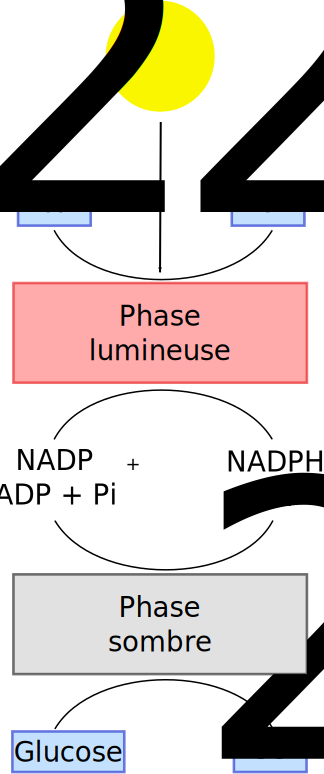
\includegraphics[scale=0.5]{img/ch2_photosynthese}
\caption{Phase lumineuse et phase sombre de la photosynthèse \cite{leninger1993principles}}
\label{photosynthese}
\end{figure}

Quoique le processus de la photosynthèse soit principalement associé à la production d'hydrates de carbone, son mécanisme fondamental consiste à capturer l'énergie lumineuse et de la transformer en énergie chimique à l'aide de pigments sensibles aux longueurs d'onde de la lumière. Ce processus prend place à l'intérieur des cellules végétales vivantes. \\

À une échelle plus fine, une cellule végétale typique possède plusieurs composantes assumant diverses fonctions. Elle est caractérisée par la présence d'une paroi cellulaire et d'une région interne qui est appelée le protoplaste. Le protoplaste est composé du cytoplasme, du noyau, d'une vacuole (qui peut atteindre 95\% du volume de la cellule), et de diverses autres substances comme des tannins, des grains d'amidon, des huiles, etc. Dans le cytoplasme, on retrouve des structures comme des chloroplastes, mitochondries, appareils de Golgi, réticulum endoplasmique, etc. \\

Les phases lumineuse et sombre de la photosynthèse se produisent toutes les deux dans les chloroplastes des cellules qui constituent donc les centrales énergétiques des cellules. La chlorophylle, le pigment donnant la couleur verte aux feuilles des plantes, est le plus important de tous les pigments impliqués dans le processus de la photosynthèse. Plusieurs types de chlorophylle peuvent être distingués, mais les plus abondants sont les chlorophylles a et b qui différencient notamment par leur spectre d'absorption de la lumière. Les chlorophylles a et b ont respectivement des maxima d'absorption dans les régions du orange-rouge et bleu-violet du spectre du visible. Le fait que les deux types de chlorophylle ne montrent que très peu d'absorption dans les longueurs d'onde du vert et du jaune (500 à 600 nm) donne la couleur caractéristique aux feuilles.\\

Plusieurs facteurs interagissent pour influencer la photosynthèse des plantes : 

\subsubsection{La quantité et la qualité de lumière}

Comme on vient de le voir, la qualité de la lumière est fort importante pour le processus de photosynthèse. Par contre, comme la lumière captée par les arbres provient du soleil, il ne s'agit pas d'un facteur facilement modifiable en conditions naturelles.\\

En revanche, la quantité de la lumière est généralement considérée comme un facteur très important pour la croissance des arbres parce qu'elle peut affecter directement le taux de photosynthèse et qu'elle peut être modifiée par des pratiques culturales. Le contrôle de la lumière est le principal outil à la disposition du sylviculteur qui veut influencer la croissance de l'arbre.\\

Les feuilles n'utilisent pour la photosynthèse qu'une petite partie de la lumière incidente. Ainsi, les feuilles sont généralement saturées en lumière à des valeurs inférieures à 50\% de la lumière incidente par temps ensoleillé (Figure~\ref{c_uptake}). 


\begin{figure}[h]
\centering
\includegraphics[scale=0.5]{img/ch2_C_uptake}
\caption{Courbe de saturation de la lumière pour différentes espèces forestières \cite{waring1985forest}. }
\label{c_uptake}
\end{figure}	

Cependant, le même phénomène n'est généralement pas observé lorsque toutes les feuilles de la cime d'un arbre sont considérées. En effet, l'ombre créée par les feuilles de la partie supérieure de la cime sur les feuilles du bas de la cime fait en sorte que peu importe l'intensité lumineuse, toutes les feuilles de la cime ne sont pas saturées en même temps. Ainsi, le taux de photosynthèse de la cime d'un arbre continue généralement d'augmenter parallèlement à l'augmentation de l'intensité de la lumière incidente et n'atteint donc pas un plateau comme dans le cas d'une feuille individuelle.\\

Par opposition au concept de saturation de la lumière, il importe aussi de souligner le point de compensation de la lumière de la lumière qui correspond à l'intensité lumineuse à laquelle le CO\sub{2} utilisé pour la photosynthèse est égal à la quantité de CO\sub{2} libéré par la respiration (voir section ~\ref{respiration}). Cette limite varie beaucoup d'une espèce à l'autre. Elle définit la tolérance à l'ombre de celles-ci (tableau~\ref{tolerance}). 

\begin{table}[h]
\centering
	
	\begin{tabular}{l c c}
	\hline
	\bf Espèce	& \bf Point de compensation & \bf Tolérance à l'ombre \\
	\hline
	\hline
	Érable à sucre & 3,4\% & Très tolérant \\
	Pruche de l'est	& 8,4\%	& Très tolérant \\
	Pin blanc &	10,4\% & Intermédiaire \\
	Chêne rouge	& 13,6\% &  Intermédiaire \\
	Pin ponderosa &	30,6\%	& Intolérant \\
	\hline
	\end{tabular}

\caption{Tolérance à l'ombre (d’après \cite{burns1990silvics}) et point de compensation (en~\% de pleine lumière du soleil d’après \cite{kimmins1987forest}) de la pour différence espèces d'Amérique du Nord }
\label{tolerance}
\end{table}

\subsubsection{La température}

Comme tous les processus métaboliques, la photosynthèse a des contraintes liées à la température qui correspondent approximativement à la tolérance des composés protéiniques (environ 0 à 60\textdegree C). D'une façon générale, une augmentation de l'activité photosynthétique est observée parallèlement à une augmentation de la température jusqu'à une température optimale. À des températures plus élevées que cette température optimale, une baisse de l'activité photosynthétique est généralement observée. Bien que le sylviculteur ne puisse avoir un impact direct sur la température régionale, il faut souligner que le contrôle de l'espacement entre les arbres a un impact sur les conditions météorologiques observées dans le couvert forestier. 

\subsubsection{L'eau}

Il est difficile d'établir si un déficit hydrique peut avoir un effet direct sur le taux de photosynthèse. En effet, la quantité réellement nécessaire pour le processus de la photosynthèse est très petite en comparaison à la quantité d'eau nécessaire pour maintenir un arbre en vie. Par conséquent, avant qu'un déficit hydrique puisse affecter directement la photosynthèse, il est très probable que des effets indirects diminuant le taux de photosynthèse se manifesteront avant.\\
 
Les effets indirects d'un déficit hydrique sur le taux de photosynthèse sont provoqués par une diminution de l'hydratation du protoplasme et par la fermeture des stomates de la feuille. À long terme, ces déficits hydriques sont issus d'une faible teneur en eau du sol associée à un faible pouvoir de rétention en eau du sol, de faibles précipitations, etc. Il est cependant à remarquer que des déficits hydriques peuvent aussi survenir à court terme (quotidiennement) lorsqu'une forte demande évaporative de l'atmosphère pendant le jour provoque une fermeture des stomates. 
 
\subsubsection{La quantité de CO\sub{2} et de O\sub{2} }

D'une part, des concentrations élevées de O\sub{2}  dans l'atmosphère peut inhiber la photosynthèse des plantes. Ce phénomène est relié à un taux de respiration plus élevé en présence de lumière.\\

D'autre part, des concentrations élevées de CO\sub{2} dans l'atmosphère augmentent l'activité photosynthétique. Comme dans le cas de la courbe de saturation à la lumière, la courbe de saturation au CO\sub{2}  comporte un point de compensation (au CO\sub{2}  cette fois) correspond à la concentration en CO\sub{2}  pour laquelle le taux de photosynthèse est égal au taux de respiration lorsque l'intensité lumineuse n'est pas limitative. 
 
\subsection{Respiration}\label{respiration}
 
La respiration est en quelque sorte le processus inverse de la photosynthèse. Toutes les cellules actives respirent continuellement, ce qui occasionne une absorption d'oxygène et une libération de CO\sub{2} dans des proportions égales. Même les cellules qui font de la photosynthèse respirent. En effet, elles aussi doivent utiliser l'énergie produite par la respiration pour alimenter leurs processus métaboliques. Une plante qui a dépassé le point de compensation à la lumière a un bilan positif de photosynthèse vs respiration.\\

La respiration est plus qu'un simple échange gazeux. C'est un processus d'oxydoréduction à l'intérieur duquel des composés sont oxydés pour former du CO\sub{2}, et l'oxygène absorbé est réduit pour former du H\sub{2}O. L'amidon, le sucrose et d'autres sucres de même que des lipides, des acides organiques et même des protéines peuvent servir de substrat pour la respiration. L'équation de la respiration dans le cas du glucose par exemple est : 

\[ C_6H_{12}O_6 + 6O_2  \longrightarrow  6CO_2 + 6H_2O + \mbox{énergie} \]

Une partie de l'énergie produite par le processus de la respiration est libérée sous forme de chaleur mais une autre partie est capturée sous forme d'ATP. L'ATP ainsi formé par la respiration peut ensuite être utilisé par la cellule pour ses différents processus métaboliques. 

\subsection{Transport des sucres} 
 
Les cellules vivantes non-photosynthétiques d'un arbre sont dépendantes des cellules photosynthétiques pour s'approvisionner en combustible organique. Cependant, la distance séparant ces deux types de cellule est parfois très grande. Par conséquent, les arbres ont besoin d'un système de translocation des sucres assez rapide et de dimension telle qu'il puisse répondre aux besoins métaboliques des cellules. Ce transport des sucres est assuré par les tubes criblés qui sont des cellules spécialisées du phloème. Ces cellules forment un réseau vasculaire pouvant transporter les sucres synthétisés par les feuilles à toutes les cellules.\\

En plus des hydrates de carbone, des composés azotés (acides aminés, amides et protéines) peuvent se retrouver dans la sève élaborée. Ces substances proviennent des feuilles ou des fruits en état de sénescence et empruntent la voie du phloème pour être relocalisées dans les tissus plus jeunes de la plante. Parmi les autres substances qu'il est aussi possible de retrouver dans la sève élaborée, il y a l'ATP, des enzymes, des ions organiques, des vitamines, des phytohormones, des herbicides, des virus, des spores de champignon, etc.\\

La direction du transport de la sève élaborée peut être latérale ou axiale. Les mouvements radiaux de la sève élaborée se font surtout vers l'extérieur lorsqu'il y a une blessure à l'écorce qui nécessite la formation d'un cal. Toutefois, des mouvements radiaux vers l'intérieur sont aussi rencontrés dans le parenchyme de rayon et ont pour but d'entreposer des sucres dans le parenchyme du xylème.\\

Par ailleurs, des études ont démontré qu'il n'y a que très peu de transport de la sève élaborée en direction tangentielle. Par exemple, une expérience a déjà démontré qu'une défoliation d'un seul côté d'un arbre aura pour effet de diminuer la croissance radiale seulement du côté où les feuilles ont été enlevées, ce qui implique que les feuilles restantes n'alimentent pas le cambium du côté défolié. Dans l'ensemble, les mouvements latéraux sont quantitativement mineurs comparativement au transport axial, i.e. du haut vers le bas ou du bas vers le haut d'un arbre.\\

Le mouvement axial de la sève élaboré n'est pas polaire, i.e. qu'il peut se produire vers le bas et vers le haut d'un arbre Figure~\ref{pomme}. 


\begin{figure}[h]
\centering
\includegraphics[scale=0.5]{img/ch2_dir_phloeme}
\caption{La croissance de pommes sur une branche annelée à deux endroits \citep{zimmerman1971trees} }
\label{pomme}
\end{figure}

Sur la Figure~\ref{pomme}, une branche de pommier a été annelée à deux endroits, ce qui a eu pour effet d'isoler la pomme b. Si le transport des sucres se faisait uniquement vers le bas de la tige, la pomme c n'aurait pas été approvisionnée en sucres, ce qui aurait diminué sa croissance. À l'inverse, si le transport des sucres se faisait uniquement vers le haut, la pomme a n'aurait pas été approvisionnée en sucres et sa croissance aurait aussi été diminuée. Puisque la croissance des pommes a et c n'a pas été réduite, il faut conclure que le transport de la sève élaborée se fait dans les deux directions.\\

La faible croissance de la pomme b prouve par ailleurs que le transport des sucres se fait bel et bien par le phloème.\\

Non seulement le mouvement axial de la sève élaborée peut se faire dans les deux directions, mais il peut se faire simultanément dans les deux directions. La Figure~\ref{phloeme} illustre ce mouvement bidirectionnel qui implique que les sucres provenant des feuilles peuvent prendre la direction des racines ou ils peuvent être mobilisés vers d'autres points de croissance comme les fleurs, les jeunes feuilles pas encore photosynthétiquement autosuffisantes, ou les fruits. 

\begin{figure}[ht]
\centering
\includegraphics[scale=0.5]{img/ch2_dir_phloeme2}
\caption{Le transport bidirectionnel de la sève élaborée \citep{zimmerman1971trees}}
\label{phloeme}
\end{figure}

D'une façon générale, il a été observé que les feuilles les plus rapprochées des racines (bas de la cime) vont principalement exporter leurs sucres vers les racines (transport vers le bas) alors que les feuilles situées près du sommet de la cime vont principalement exporter leurs sucres vers le haut. Les sucres des feuilles dans une situation intermédiaire seront transportés dans les deux directions.\\ 

À partir d'expériences avec des isotopes radioactifs, il a été possible d'évaluer que la vitesse de transport de la sève élaborée dans le phloème se situait entre 10 et 100 cm/heure, ce qui est remarquablement grand en considérant la taille relativement petite du complexe de tubes criblés qui compose le phloème. Plusieurs hypothèses ont été élaborées pour tenter d'expliquer le mécanisme de transport dans le phloème, mais personne n'a jusqu'ici prouvé qu'une de ces théories était hors de tous doutes le véritable mécanisme. L'étude de ces théories dépasse le cadre de ce cours.\\

\subsection{Transport de l'eau}\label{eau}

Le transport de l'eau brute prend place dans le xylème de l'arbre, ce qui implique qu'il a un important impact sur l'utilisation et la transformation du bois. Physiologiquement, l'aubier représente la partie du xylème qui sert au transport de l'eau (et à l'entreposage des sucres). Tel que présenté au tableau~\ref{humidite}, cette partie de l'arbre a une teneur en humidité beaucoup plus élevée puisque le lumen de ses cellules contiennent de l'eau.\\ 

La force permettant à l'eau de se déplacer du sol jusqu'au sommet d'un arbre est fournie par le gradient de potentiel hydrique entre le sol et l'atmosphère. Puisque l'eau se déplace d'un endroit à fort potentiel vers un endroit à faible potentiel, il faut donc que le potentiel hydrique de l'atmosphère soit plus bas que celui du sol. Cette condition est généralement remplie parce que sous des conditions normales d'humidité relative de l'atmosphère, l'air a un potentiel hydrique beaucoup plus bas que celui du sol. \\

Le faible potentiel hydrique de l'atmosphère généralement rencontré en condition normale fait en sorte que l'eau des feuilles est attirée vers l'atmosphère, et l'évaporation de l'eau qui survient alors à la surface des feuilles est appelé transpiration. À cause de ce phénomène de transpiration, la teneur en eau des cellules foliaires est diminuée, ce qui provoque une baisse de leur potentiel hydrique.\\  

Cette baisse du potentiel hydrique des feuilles aura pour conséquence d'établir un gradient de potentiel hydrique entre les feuilles et le xylème des branches, ce qui aura pour résultat de créer un mouvement d'eau des branches jusqu'aux feuilles.\\ 

En peu de temps, le gradient de potentiel hydrique s'établira partout dans la plante (des feuilles aux racines) et s'étendra finalement jusqu'au sol entourant les racines pour permettre l'entrée de l'eau du sol dans les racines. Ainsi, le gradient de potentiel hydrique qui s'établit entre le sol et l'atmosphère permet aux arbres de puiser l'eau dans le sol et de la retourner dans l'atmosphère par l'entremise de leurs feuilles.\\

Les forces d'adhésion et de cohésion de l'eau sont d'autres propriétés conférant à l'eau une très grande importance pour les plantes.\\

À cause de sa nature polaire (charge positive à une extrémité d'une molécule d'eau et charge négative à l'autre extrémité), l'eau est attirée par plusieurs autres substances, comme les protéines et la cellulose, et les imbibe. Cette attraction entre l'eau et d'autres substances est appelée adhésion.\\

Par ailleurs, l'attraction exercée par les molécules d'eau entre elles est appelée cohésion. Cette force de cohésion entre les molécules d'eau est responsable de la grande résistance de l'eau à la tension et fait en sorte qu'une colonne d'eau de petit diamètre (comme dans une trachéide ou un vaisseau) peut résister à l'application de très fortes tensions. C'est donc cette force de cohésion qui permet à l'eau d'être transportée des racines jusqu'aux feuilles d'un arbre.\\

Chez les gymnospermes (arbres résineux), le transport de l'eau est assuré par des trachéides qui ne sont pas ouvertes à leurs deux extrémités comme les éléments de vaisseau mais qui comportent plusieurs ponctuations principalement concentrées aux deux bouts des trachéides. Puisqu'un certain chevauchement existe entre les trachéides, l'eau peut monter jusqu'au sommet d'un arbre en passant d'une trachéide à l'autre via les ponctuations.\\ 

Puisque les trachéides ont un plus petit diamètre que les vaisseaux et ne sont pas ouvertes à leurs deux extrémités, le transport de l'eau rencontre plus de résistance dans le bois de conifères comparativement aux angiospermes (arbres feuillus). Chez les angiospermes, le transport de l'eau se fait plus rapidement chez les espèces ayant du bois à zones poreuses (ex. : chênes, frênes, orme) que celles possédant du bois à pores diffus (ex. : érables, peupliers, bouleaux).\\

Parmi les autres propriétés de l'eau, il est important de noter que l'eau est un solvant pour plusieurs substances et peut donc servir de véhicule aux acides aminés, aux hydrates de carbone de faible poids moléculaire, aux ions (K+, Ca+2, H2PO4, NO3-, etc.) et à de petites molécules sous forme gazeuse comme l'oxygène. Cette propriété de l'eau, conjointement avec sa force de cohésion, permet donc le transport des éléments minéraux des racines jusqu'aux feuilles.\\ 

\subsection{La nutrition minérale}

Bien que la plante soit principalement formée de matière organique (les composés C, H et O forment ensemble 95\% de la masse anhydre d'une plante), elle a également besoin de nombreux éléments inorganiques puisés dans le sol pour accomplir ses différentes fonctions métaboliques. La Figure~\ref{mineraux} montre la forme de la relation entre la croissance d'une plante et sa concentration en éléments minéraux. 

\begin{figure}[h]
\centering
\includegraphics[scale=1]{img/ch2_nutr_min}
\caption{Relation entre la croissance d'une plante et sa concentration en éléments minéraux \citep{landis1989container}}
\label{mineraux}
\end{figure}

En dépit du nombre élevé d'éléments disponibles dans le sol et rencontrés dans les analyses chimiques des plantes, les physiologistes ne reconnaissent actuellement que 16 éléments minéraux indispensables à la croissance de la plupart des plantes. Les éléments essentiels se divisent arbitrairement en deux groupes : les éléments majeurs ou macroéléments qui sont requis en grande quantité (20 à 1000 mg/litre de solution), et les éléments mineurs ou oligoéléments qui sont requis en très petites quantité (<10 mg/litre). La liste de ces éléments est donnée au tableau~\ref{elements}. 

\begin{table}[h]
\centering
	
	\begin{tabular}{l c c}
	\hline
	& \bf Forme d'absorption & \bf Concentration (ppm) \\
	\hline
	\hline
	H & H\sub{2}O &  \numprint{60000} \\
	C &  CO\sub{2}&  \numprint{450000} \\
	O & CO\sub{2}, H\sub{2}O, O\sub{2} & \numprint{450000}  \\
	N &  & \numprint{15000} \\
	K & K\up{+} & \numprint{10000} \\
	Ca & Ca\up{2+} & \numprint{5000} \\
	Mg & Mg\up{2+}  & \numprint{2000} \\
	P &  & \numprint{2000} \\
	S & SO\sub{4} &  \numprint{1000} \\
	\hline
	Cl & Cl\up{-} & 100 \\
	B &  &  20 \\
	Fe &  & 100  \\
	Mn & Mn\up{2+} & 50 \\
	Zn & Zn\up{2+} & 20 \\
	Cu & Mg\up{2+}  & 6 \\
	Mo &  & 0.1 \\
	\hline
	\end{tabular}

\caption{Liste des éléments essentiels à toutes les plantes vasculaires et concentration dans les tissus}
\label{elements}
\end{table}

\subsection{La régulation de la croissance par les hormones}

À partir d'observations et d'expériences, certains chercheurs ont suggéré que des substances chimiques régularisant la croissance étaient présentes dans les plantes. Cette théorie a été proposée pour la première fois par le botaniste allemand Sachs vers la fin du 19e siècle et a été suivie par de nombreuses études qui se poursuivent encore de nos jours.\\

Au fil de ces recherches, une terminologie s'est établie de façon à pouvoir distinguer les substances impliquées dans la régulation de la croissance des végétaux. Ainsi, une phytohormone est définie comme étant un composé organique synthétisé par une certaine partie d'une plante et généralement transporté vers une autre partie de cette plante où, à de très faibles concentrations, il régularise un processus physiologique.\\ 

Cinq groupes de phytohormones jouent des rôles importants dans la physiologie des arbres. Il s'agit des auxines, des gibbérellines, des cytokinines, de l'acide abscissique et de l'éthylène. Parmi celles-ci, les auxines revêtent une importance particulière pour l'anatomie et la structure du bois. 

\subsection{Les auxines}\label{section_auxines} 

Les auxines sont un groupe de substances de structure voisine à l'acide indole 3 acétique (AIA) qui est la plus répandue des auxines naturelles. La découverte des auxines s'est faite en plusieurs étapes. Le premier scientifique qui a contribué à cette découverte fut Darwin qui est mieux connu pour sa théorie de l'évolution que pour ses travaux sur les auxines. Il a démontré que l'inclinaison des tiges et des racines d'une plante en présence d'une source de lumière unidirectionnelle était contrôlée par l'apex. Cette inclinaison des plantes vers la lumière est appelée phototropisme. Darwin a aussi observé que lorsque l'apex de la plante était coupé ou couvert, aucune inclinaison de la plante ne se produisait.\\

Il est possible de retrouver des auxines partout dans une plante mais les plus fortes concentrations se rencontrent dans les apex, les méristèmes et les jeunes feuilles des bourgeons terminaux où ils sont synthétisés. Les plus fortes concentrations d'auxines sont donc rencontrées dans le haut des tiges. En allant vers le bas de la tige, il y a normalement une diminution graduelle de la concentration d'auxines qui est suivie par une augmentation au niveau de la pointe des racines. Un précurseur primaire de l'AIA est le tryptophane qui est un acide aminé. \\

Outre le phototropisme, les auxines régulent plusieurs processus dont notamment la dominance apicale, la production du péricarpe des fruits, l'abscission des feuilles à l'automne, la production racinaire, la formation de cals pour cicatriser les blessures, l'élongation cellulaire et le géotropisme.\\

Les deux derniers éléments de cette énumération montrent que les auxines jouent un rôle primordial pour déterminer les caractéristiques du bois produit par un arbre. La théorie expliquant l'effet de la sylviculture sur la qualité du bois est d'ailleurs centrée sur la concentration de ces hormones dans la plante. Cette théorie, développée par \cite{larson1969wood} sera abordée en détails au chapitre 8.\\

Pour mettre en évidence le lien entre les auxines et la qualité du bois, on peut utiliser le mécanisme par lequel le mode de croissance des plantes est affecté par la force de gravité (le géotropisme). Quand une plante est mise en position horizontale, sa croissance sera déviée de façon à ce que la tige soit dirigée vers le haut (géotropisme négatif) et les racines vers le bas (géotropisme positif). Pour pouvoir orienter sa croissance vers le haut, il faut que la croissance des cellules de la face inférieure de la tige soit plus rapide que celle des cellules de la face supérieure. Cette différence de croissance est possible par une augmentation de la concentration d'auxines dans les cellules de la partie inférieure de la tige qui se ferait à cause de la gravité. On remarque donc qu'une concentration plus élevée d'auxines entraine une activité cambiale plus élevée. \\

C'est par ce même processus que les conditions de croissance affectent le défilement d'une tige. Les arbres croissant en lieux ouverts et n'ayant pas subi d'élagage artificiel ont généralement des branches sur toute la longueur de la tige. À l'opposé, les arbres croissant sous couvert ou ayant subi un élagage artificiel ont moins de branches. Dans un tel cas, la concentration en auxines produites dans les méristèmes apicaux se veut beaucoup plus élevée dans le haut de la tige (tel qu'illustré à la Figure~\ref{auxines}). Comme ces hormones agissent comme démarreur de l'activité cambiale, la croissance en diamètre débute plus rapidement dans la cime vivante au printemps. De plus, la concentration en auxines demeure plus élevée dans la cime vivante tout au long de la saison de croissance, ce qui stimule davantage l'activité cambiale dans cette partie de la tige. Le défilement de la tige est donc moins fort (tige plus cylindrique) pour les arbres possédant une cime vivante moins développée, c'est-à-dire les arbres croissant sur des sites de densité de peuplement plus élevée ou les arbres ayant subi un élagage artificiel. Il est également à remarquer que du bois de type juvénile est produit sous l'effet d'une concentration élevée en auxines, donc dans la cime vivante.  

\begin{figure}[h]
\centering
\includegraphics[scale=0.5]{img/ch2_auxine}
\caption{Impact de l'importance de la cime vivante sur le défilement de la tige (adapté de \cite{jozsa1994discussion}. Image préparée par Julie Ferland pour \cite{achim2010dendroecologie}}
\label{auxines}
\end{figure}

% 
%Références 
%Burns, R.M., Honkala, B.H. 1990. Silvics of North America. 654, Vol. 1 Conifers., USDA For. Serv. 675 p. 
%Jozsa, L.A.; Middleton, G.R. 1997. Les caractéristiques determinant la qualité du bois : Nature et conséquences pratiques. Publication spéciale SP-34F, Forintek Canada Corp., Québec. 42 p. 
%Haygreen, J.G.; Bowyer, J.L. 1989. Forest products and wood science. An introduction. Second Edition. Iowa State University Press. Ames, USA. 500 p. 
%Hoadley, R.B. 1990. Identifying wood. Accurate results with simple tools. The Taunton Press Inc. Connecticut, USA. 223 p. 
%Kimmins, J.P. 1987. Forest ecology. Macmillan Publishing Company, New York, U.S.A. 
%Landis, T.D., Tinus, R.W., McDonald, S.E. et Barnett, J.P. 1989. The container tree nursery manual. Volume Four. Seedling nutrition and irrigation. Agric. Handb. 674. USDA For. Serv., Washington, D.C., U.S.A. 
% 
%Larson, P. 1969: Wood formation and the concept of wood quality. Yale Univ. Sch. For. Bull. 74: 1-54. 
%Lehninger, A.L. 1982. Principles of biochemistry. Worth Publishers Inc., New York, U.S.A. 
%MRNF. 2007. Ressources et industries forestières – Édition complète. Ministère des ressources naturelles et de la faune, Gouvernement du Québec. 
%Panshin, A.J.; de Zeeuw, C. 1980. Textbook of wood technology. Fourth edition. McGraw-Hill Book Co. New York. 722 p. 
%Waring, R.H. and Schlesinger, W.H. 1985. Forest ecosystems, concepts and management. Academic Press, London, U.K. 
%Weier, T.E.; Stocking, C.R.; Barbour, M.G. 1974. Botany: An introduction to plant biology. Fifth edition. John Wiley and Sons. New York. 693 p. 
%Zimmermann, M.H. et Brown, C.L. 1971. Trees structure and function. Springer-Verlag, Berlin, Germany. 
% 
% 

\chapter{Description microscopique des bois résineux}\label{resineux}

\begin{abstract}
Ce chapitre décrit chacun des types de cellules rencontrés chez les arbres résineux. Nous nous attardons aussi à certaines caractéristiques anatomiques, comme les ponctuations des champs de croisement, qui permettent d'identifier les espèces.
\end{abstract}

\minitoc

\section{Introduction}

La caractéristique essentielle du bois des résineux (gymnospermes) est l'absence de cellules spécialisées pour la conduction de la sève brute tel qu'on en retrouve chez les feuillus. La sève brute circule par les trachéides longitudinales qui jouent à la fois un rôle de support mécanique et de conduction.\\

Le bois des résineux possède une structure simple composée essentiellement de trois types de cellules :

\begin{enumerate}
\item Les trachéides longitudinales;
\item Les trachéides transversales;
\item Les parenchymes :
	\begin{itemize}
	\item Parenchyme de rayon;
	\item Cellules épithéliales;
	\item Parenchyme longitudinal
	\end{itemize}
\end{enumerate}

\section{Cellules orientées longitudinalement}

\subsection{Trachéides longitudinales}

Les trachéides longitudinales sont les plus longues cellules que l'on retrouve chez les bois résineux et feuillus. Elles représentent environ 92\% du volume du bois. Elles ont deux fonctions principales, soit le support mécanique de la tige et la conduction de la sève brute. Leur longueur varie de 3 à 7 mm environ en fonction des espèces (voir Tableau~\ref{tab:diam_long}).\\

En plan transversal, les trachéides longitudinales sont disposées en files radiales. Ceci est spécifique aux résineux, les feuillus présentant une disposition plutôt aléatoire. Cette disposition en files radiales s'explique par le fait que le diamètre tangentiel des trachéides longitudinales change peu ou pas, du bois initial au bois final. Par contre, le diamètre radial des trachéides diminue du bois initial au bois final et l'épaisseur des parois cellulaires augmente. La section des trachéides longitudinales est de forme plutôt hexagonale dans le bois initial et de forme rectangulaire dans le bois final.

\begin{table}[ht]
\centering
	
	\begin{tabular}{l c c}
	\hline
	\bf Espèce	& \bf $\varnothing$ tangentiel (\micro m)& \bf Longueur (mm) \\
	\hline\hline
	Séquoia (\textit{Sequoia sempervirens}) & 50-80 & 7.0 \\
	Pin à encens (\textit{Pinus taeda})  &  35-60 &  4.3\\
	Sapin Douglas (\textit{Pseudotsuga menziesii})  & 35-55 & 3.4 \\
	Sapin baumier (\textit{Abies balsamea})  & 30-50 & 3.3 \\
	Pin blanc \textit{(Pinus strobus})  & 25-45 &  3.5 \\
	Mélèze laricin (\textit{Larix laricina})  & 30-45 & 3.0 \\
	Épinette noire (\textit{Picea mariana})  & 25-30 & 3.5 \\
	Épinette blanche (\textit{Picea glauca})  & 25-35 & 3.3 \\
	Genévrier rouge (\textit{Juniperus virginiana})  & 20-35 & 2.2 \\
	If de l'Ouest (\textit{Taxus brevifolia}) & 15-25 &  2.3\\
	\hline
	\end{tabular}

\caption{\label{tab:diam_long} Dimensions des trachéides de quelques bois résineux (d'après \cite{panshin1980textbook}}
\end{table}

La transition du bois initial au bois final varie en fonction des espèces. Par exemple, elle est graduelle chez l'épinette (\textit{Picea spp.}) et abrupte chez le sapin Douglas (\textit{Pseudotsuga menziesii}) (Figure~\ref{transition}).

\begin{figure}[h]
\centering
\includegraphics[scale=0.6]{img/ch3_transition}
\caption{Illustration de la différence entre une transition abrupte chez le Douglas (\textit{Pseudotsuga menziesii}) et graduelle chez l'épinette (\textit{Picea spp.}) (grossissement : $\times$40) du bois initial au bois final. Image préparée par Julie Ferland pour \cite{achim2010dendroecologie}}
\label{transition}
\end{figure}

\subsubsection{Dimensions des trachéides longitudinales}

Le diamètre tangentiel des trachéides est un caractère héréditaire, donc peu variable à l'intérieur d'une espèce. Ce caractère défini les bois résineux à texture fine ou grossière (Figure~\ref{fig:texture}). Par exemple, le bois de séquoia présente une texture grossière avec des trachéides longitudinales d'un diamètre tangentiel moyen d'environ 80 \micro m. À l'opposé, le bois du if de l'Ouest (\textit{Taxus brevifolia}) a une texture fine avec des trachéides longitudinales d'un diamètre tangentiel moyen d'environ 25 \micro m. Plusieurs bois résineux commerciaux ont une texture moyenne avec des trachéides longitudinales d'un diamètre tangentiel variant de 30 à 45 \micro m (Tableau~\ref{tab:diam_long}). On remarque que la longueur des trachéides longitudinales est généralement corrélée avec le diamètre tangentiel, c'est-à-dire que les bois à texture grossière possèdent également les plus longues trachéides longitudinales.

\subsubsection{Épaississements spiralés}

Les épaississements spiralés sont des épaississements de la paroi tertiaire (S\sub{3}) des trachéides, disposés du côté du lumen (Figure~\ref{fig:epaississ}). Ils sont toujours présents chez les trachéides longitudinales et transversales du bois de sapin Douglas et sont utilisés comme critère d'identification pour cette espèce.\\

L'angle que font les épaississements avec l'axe longitudinal de la trachéide est approximativement le même que celui des microfibrilles de la paroi S\sub{3}. On distingue les épaississements en \og S \fg  et les épaississements en \og Z \fg  en fonction de l'orientation de la spirale lorsqu'on l'observe en plan longitudinal-radial ou longitudinal-tangentiel. 

%image à refaire avec une meilleure résolution
\begin{figure}[h]
\centering
\includegraphics[scale=0.7]{img/texture}
\caption{De gauche à droite : Bois à texture grossière (séquoia); bois à texture moyenne (sapin baumier); bois à texture fine (épinette) (grossissement $\times$40).}
\label{fig:texture}
\end{figure}

\begin{figure}[h]
\centering
\includegraphics[scale=1]{img/epaississements}
\caption{Épaississements spiralés en S chez le sapin Douglas (\textit{Pseudotsuga menziesii}) (tiré de \cite{butterfield2012three}; grossissement $\times$850)}
\label{fig:epaississ}
\end{figure}

\subsection{Files de trachéides}

Les files de trachéides sont constituées de courtes trachéides longitudinales dotées de parois terminales. Elles possèdent des ponctuations aréolées, ce qui permet de les différencier des parenchymes longitudinaux. Ces trachéides courtes peuvent être considérées comme des cellules transitoires entre les trachéides longitudinales d'une part et les parenchymes longitudinaux et les cellules épithéliales d'autre part. Lorsqu'elles sont présentes, les files de trachéides sont souvent situées au voisinage des canaux résinifères, à la marge des cernes annuels ou au voisinage des canaux résinifères traumatiques. En Amérique du Nord, on les retrouve parfois chez les mélèzes (\textit{Larix spp.}) (Figure~\ref{fig:file}), le sapin Douglas et le séquoia (\textit{Sequoia sempervirens}).

\subsection{Parenchymes orientés longitudinalement}

Les parenchymes sont des cellules ayant pour fonction la sécrétion des résines ou la réserve de substances nutritives. Leur paroi cellulaire a une structure différente de celle des trachéides puisqu'on a soit une paroi primaire mince, soit une paroi primaire épaissie qui a l'allure d'une paroi secondaire. On rencontre deux types de parenchymes orientés longitudinalement chez les résineux : 1) le parenchyme longitudinal et 2) le parenchyme épithélial (ou cellules épithéliales).

\begin{figure}[h]
\centering
\includegraphics[scale=0.2]{img/file}
\caption{File de trachéides chez le mélèze de l'Ouest (\textit{Larix occidentalis}) (adapté de \cite{panshin1980textbook}}
\label{fig:file}
\end{figure}

\subsubsection{Parenchyme longitudinal}

Contrairement aux feuillus, le parenchyme longitudinal n'est pas très fréquent ni abondant chez les résineux. On le rencontre toutefois chez certaines espèces où il prend la forme de files orientées longitudinalement. Il sert alors de tissu de réserve. Comme c'est toujours le cas entre les parenchymes, les ponctuations sont simples au niveau des parois terminales, c'est-à-dire à l'interface entre deux cellules de parenchyme. Les parois terminales sont dites lisses ou noduleuses selon que les ponctuations simples forment des nodules ou non.\\

Le parenchyme longitudinal n'est jamais présent chez le genre \textit{Pinus}. Il est sporadiquement présent chez les genres \textit{Larix}, \textit{Pseudotsuga}, \textit{Tsuga} et \textit{Abies}. Il est relativement abondant chez les genres de la famille des Cupressaceae (\textit{Thuja, Chamaecyparis, Cupressus, Calocedrus,} et \textit{Juniperus}). Toutefois, il est abondant chez les genres de la famille des Taxodiaceae (\textit{Sequoia} et \textit{Taxodium}). Le parenchyme longitudinal chez le séquoia est présenté à la figure~\ref{fig:par_long}.\\

\subsection{Parenchyme épithélial et canaux résinifères longitudinaux}

Les cellules de parenchyme épithélial sécrètent la résine chez les résineux. Elles recouvrent les canaux résinifères longitudinaux et transversaux des bois résineux qui en possèdent. Un canal résinifère est en réalité un espace intercellulaire, c'est-à-dire une cavité recouverte de cellules épithéliales. Les cellules épithéliales forment l'épithélium qui peut avoir plusieurs cellules d'épaisseur. L'épaisseur des cellules épithéliales varie d'une espèce à l'autre. On les qualifie de cellules épithéliales à paroi mince (Figure~\ref{fig:epth_mince}) ou de cellules épithéliales à paroi épaisse (Figure~\ref{fig:epth_epaisse}). Le tableau~\ref{tab:mince_epaisse} présente les principales caractéristiques de quelques bois résineux d'Amérique du Nord en ce qui concerne les canaux résinifères.


\begin{figure}[h]
\centering
\includegraphics[scale=0.7]{img/parenchyme_long}
\caption{Parenchyme longitudinal à parois terminales lisses en coupe longitudinale-tangentielle chez le séquoia (\textit{Sequoia sempervirens}) (grossissement $\times$100).}
\label{fig:par_long}
\end{figure}

\begin{figure}[h]
\centering
\includegraphics[scale=0.7]{img/epith_mince}
\caption{Canal résinifère longitudinal et cellules épithéliales à paroi mince chez le pin blanc (\textit{Pinus strobus}) (grossissement $\times$100)}
\label{fig:epth_mince}
\end{figure}


\begin{figure}[h]
\centering
\includegraphics[scale=0.7]{img/epith_epaisse}
\caption{Canal résinifère longitudinal et cellules épithéliales à paroi épaisse chez l'épinette \textit{(Picea spp.)} (grossissement : $\times$400)}
\label{fig:epth_epaisse}
\end{figure}

\begin{table}[ht]
	\centering
	
	\begin{tabular}{l c c}
		\hline
		\bf Sans canaux résinifères normaux	& \multicolumn{2}{c}{\textbf{Avec canaux résinifères normaux}}\\
		& \bf cell. épith. à parois minces & \bf cell. épith. à parois épaisses\\
		\hline\hline
		Pruches \textit{(Tsuga spp.)} &	Pins \textit{(Pinus spp.)} &	Épinettes \textit{(Picea spp.)}\\
		Sapins \textit{(Abies spp.)} & & Mélèzes \textit{(Larix spp.)}\\
		Genévrier rouge \textit{(J. virginiana)} & & Sapin Douglas \textit{(P. menziesii)}\\
		Séquoia \textit{(Sequoia sempervirens)} &&\\
		Thuyas \textit{(Thuja spp.)}&&\\
		\hline
	\end{tabular}
	
	\caption{\label{tab:mince_epaisse} Présence ou absence des canaux résinifères normaux chez quelques bois résineux d’Amérique du Nord}
\end{table}

Les cellules épithéliales à paroi mince et à paroi épaisse présentent certaines particularités. Les cellules épithéliales à paroi mince des pins n'ont pas de ponctuations et ne sont pas lignifiées. Les cellules épithéliales à paroi épaisse des épinettes, des mélèzes et du sapin Douglas ont des ponctuations et sont lignifiées.

\subsection{Canaux résinifères normaux ou traumatiques}

Les canaux résinifères sont qualifiés de normaux ou de traumatiques. Les canaux résinifères normaux sont toujours présents chez les espèces où ils sont caractéristiques. Ces canaux résinifères sont présents en direction longitudinale et en direction radiale dans les rayons fusiformes.\\

Les canaux résinifères traumatiques apparaissent chez des arbres ayant subi une blessure mécanique du cambium, une attaque d'insectes ou toute autre source de stress. Ils peuvent être transversaux ou longitudinaux mais rarement les deux pour un échantillon donné. Ils peuvent être présents chez des espèces qui n'ont pas de canaux résinifères normaux comme les pruches et les sapins. Les cellules épithéliales des canaux résinifères traumatiques sont toujours à paroi épaisse et sont lignifiées.

\section{Cellules orientées transversalement}

On rencontre trois types de cellules orientées transversalement dans le xylème des résineux qui sont toutes présentes des les rayons ligneux: 1) les parenchymes de rayon; 2) les trachéides transversales et 3) les cellules épithéliales.

\subsection{Parenchymes de rayon et rayons ligneux}

Les cellules des parenchymes de rayon ont des parois cellulaires minces. Il s'agit de paroi primaire plus ou moins épaissie. Les ponctuations entre ces cellules sont de type simple. Les ponctuations du plan longitudinal-radial des parenchymes de rayon en contact avec les trachéides longitudinales sont appelées champs de croisement (Figure~\ref{fig:croisement}). La forme des ponctuations semi-aréolées que l'on retrouve dans les champs de croisement est importante pour l'identification des bois résineux.\\

Les parenchymes de rayon forment les rayons qui sont disposés en direction radiale. Les cellules de parenchyme de rayon du bois d'aubier sont vivantes et celles du bois de duramen sont mortes. Les rayons ligneux traversent le xylème et le phloème et sont utilisés pour le transport de la sève élaborée du phloème vers les parenchymes vivants de l'aubier. Les rayons ligneux ne contenant qu'une cellule de large en plan longitudinal-tangentiel sont dits unisériés. Si on a deux cellules de large, on a alors des rayons ligneux bisériés. Dans la plupart des cas, les rayons sont unisériés chez les résineux. La hauteur des rayons varie entre les espèces. Elle est de 40 à 60 cellules de hauteur (0,5 à 1 mm) chez le séquoia, de 10 à 15 cellules en moyenne et peut descendre à moins de 6 cellules (0,3 mm) chez le genévrier. Le volume moyen des rayons est d'environ 7\% du volume total du bois chez les résineux.

\begin{figure}[h]
	\centering
	\includegraphics[scale=0.8]{img/ch3_croisement}
	\caption{Le champs de croisement sont constitués par l'interface entre des cellules de rayon et des trachéides dans le plan longitudinal-radial. Image préparée par Julie Ferland pour \cite{achim2010dendroecologie}}
	\label{fig:croisement}
\end{figure}

\subsection{Trachéides transversales et rayons fusiformes}

Les trachéides transversales sont présentes chez plusieurs résineux. Ce sont des cellules mortes orientées radialement et associées aux rayons ligneux. Elles possèdent des ponctuations aréolées tout comme les trachéides longitudinales, mais de plus petit diamètre. C'est d'ailleurs grâce à leurs paires de ponctuations aréolées qu'on peut facilement les distinguer des parenchymes de rayon (Figure~\ref{fig:trach_trans}).\\

Les trachéides transversales sont présentes chez les pins, les épinettes, les mélèzes, les pruches et le sapin de Douglas. On les retrouve sporadiquement chez les sapins et très rarement chez le séquoia, les thuyas et les genévriers.\\

Les trachéides transversales sont lisses ou dentées. Les trachéides transversales dentées (Figure~\ref{fig:dentees}) sont caractéristiques des groupes des pins durs (\textit{Pinus banksiana, Pinus resinosa, Pinus ponderosa}) et des pins du Sud (\textit{Pinus palustris, Pinus echinata, Pinus taeda, Pinus elliottii, Pinus rigida, Pinus serotina}, etc.).\\

Les parenchymes de rayon et le cas échéant les trachéides transversales vont parfois être associés à des canaux résinifères transversaux. Dans ce cas, on désigne cette structure comme étant un rayon fusiforme. On peut observer les rayons fusiformes en plan longitudinal-tangentiel (Figure~\ref{fig:fusiforme}). Ils permettent de s'assurer qu'il s'agit bien d'un bois possédant des canaux résinifères, car les canaux résinifères transversaux sont invariablement présents dans ce cas. Les rayons fusiformes contiennent donc les trachéides transversales, le parenchyme de rayon et les cellules épithéliales du ou des deux canaux résinifères présents.

\begin{figure}[h]
	\centering
	\includegraphics[scale=0.8]{img/ch3_Fahn_trach}
	\caption{Portion du plan longitudinal-radial d’un bois résineux montrant les parenchymes de rayon, les champs de croisement et les trachéides transversales (adapté de \cite{fahn1990plant})}
	\label{fig:trach_trans}
\end{figure}

\begin{figure}[h]
\centering
\includegraphics[scale=0.7]{img/ch3_dentees}
\caption{Trachéides transversales dentées en plan longitudinal-radial chez Pinus radiata (tiré de Butterfield et Meylan 1980) (grossissement : $\times$1500)}
\label{fig:dentees}
\end{figure}

\begin{figure}[h]
\centering
\includegraphics[scale=0.8]{img/ch3_fusiforme}
\caption{Rayon fusiforme en plan longitudinal-tangentiel chez l'épinette (Picea spp.) (Grossissement : $\times$400)}
\label{fig:fusiforme}
\end{figure}

Le nombre de rayons fusiformes est toujours inférieur au nombre de rayons unisériés. Par exemple, le ratio est de 1:25 chez le sapin Douglas, 1:40 chez les épinettes et 1:60 chez les mélèzes.\\

Les rayons unisériés sont dits homo-cellulaires s'ils ne sont constitués que de parenchymes de rayon ou que de trachéides transversales. Ils sont dits hétérocellulaires s'ils sont constitués d'un mélange des deux types de cellules.

\section{Ponctuations} %ajoute rimage comme au chapitre 4

Les ponctuations peuvent être définies comme une discontinuité dans la paroi cellulaire donnant naissance à une ouverture. Elles se présentent généralement deux à deux pour former une paire de ponctuations entre deux cellules servant au passage des liquides dans l'arbre vivant.
%
\subsection{Ponctuations parenchyme - parenchyme}

Les ponctuations que l'on retrouve entre les parenchymes et en particulier, entre les parenchymes de rayon, sont des paires de ponctuations simples (Figure~\ref{fig:ponctuations2}A).

\subsection{Ponctuations trachéide - trachéide}

Les ponctuations que l'on retrouve entre les trachéides sont des paires de ponctuations aréolées (Figure~\ref{fig:ponctuations2}B). Les paires de ponctuations inter-trachéales sont les plus nombreuses et les plus grosses sur les parois radiales des trachéides du bois initial. On peut avoir plus d'une ponctuation de large sur la face radiale des trachéides longitudinales : 

\begin{itemize}
\item texture fine (épinettes):	ponctuations unisériées;
\item texture moyenne (pins):	ponctuations bisériées;
\item texture grossière (séquoia):	3 à 4 ponctuations de large.
\end{itemize}

Les crassules sont des lignes foncées apparaissant sur les faces radiales des cellules autour des paires de ponctuations bisériées. Les ponctuations sur les parois tangentielles sont plus petites que sur les parois radiales et ne sont présentes que pour les dernières rangées de cellules du bois final. 

\subsection{Ponctuations trachéide - parenchyme}

Les ponctuations que l'on retrouve entre les trachéides et les parenchymes sont des paires de ponctuations semi-aréolées (Figure~\ref{fig:ponctuations2}C). Les ponctuations des champs de croisement sont de ce type et ont une importance particulière pour l'identification des bois de résineux. On distingue 5 types de ponctuations des champs de croisement qui sont illustrés à la figure~\ref{fig:ponctuations} et décrits ci-dessous. La figure~\ref{fig:pontuations_cote} montre des coupes de chacune de ces ponctuations qui pourront vous aider à comprendre ce que vous observerez au microscope.

\begin{figure}[h]
\centering
\includegraphics[scale=0.7]{img/ch3_ponctuations2}
\caption{Ponctuations (A) simples (B) aréolées; (C) semi-aréolées; Image préparée par Julie Ferland pour \cite{achim2010dendroecologie}}
\label{fig:ponctuations2}
\end{figure}


\begin{figure}[h]
	\centering
	\includegraphics[scale=0.7]{img/ch3_ponctuations}
	\caption{Ponctuations des champs de croisement. Image préparée par Julie Ferland pour \cite{achim2010dendroecologie}}
	\label{fig:ponctuations}
\end{figure}
	
\subsubsection{Ponctuations fenestriformes}

Grandes ponctuations de forme quadrangulaire présentes chez certains pins (pin blanc et pin rouge par exemple).

\subsubsection{Ponctuations pinoïdes}

Ponctuations plus petites que les ponctuations fenestriformes et plus nombreuses par champs de croisement. L'aréole peut ne pas être visible dans le bois initial. Elles sont caractéristiques du groupe des pins durs.

\subsubsection{Ponctuations picéoïdes}

Petites ponctuations à ouverture étroite, linéaire et semblant déborder l'aréole. Elles sont caractéristiques des épinettes, des mélèzes, du sapin Douglas et des pruches.

\subsubsection{Ponctuations taxodioïdes}

Ponctuations à ouverture ovale à circulaire tangente en deux points au contour de l'aréole. L'aréole est étroite mais bien visible. Elles sont caractéristiques du séquoia, des sapins et des thuyas.

\subsubsection{Ponctuations cupressoïdes}

Ponctuations semblables aux picéoïdes mais l'ouverture est elliptique et entièrement incluse dans l'aréole. Elles sont caractéristiques du genévrier, des cyprès (\textit{Chamaecyparis spp.}) et présentes à l'occasion chez les épinettes et les pruches.

\begin{figure}[h]
	\centering
	\includegraphics[scale=0.6]{img/ch3_pontuations_cote}
	\caption{Ponctuations des champs de croisement en plan tangentiel a) fenestriformes; b) pinoïdes; c) picéoïdes; d) cupressoïdes; e) taxodioïdes; (d’après \cite{butterfield2012three})}
	\label{fig:pontuations_cote}
\end{figure}

\section{L'anatomie du bois des résineux en un clin d'œil}

La figure~\ref{fig:Fahn} illustre l'organisation des différentes cellules du bois des résineux.

\begin{figure}[h]
\centering
\includegraphics[scale=0.7]{img/ch3_Fahn}
\caption{Structure tridimensionnelle générale des résineux (adapté de \cite{fahn1990plant})}
\label{fig:Fahn}
\end{figure}




%Références
%
%Butterfield, B.G.; Meylan, B.A. 1980. Three-dimensional structure of wood. An ultrastructural approach. Second edition. Chapman and Hall, London, New York. 103 p.
%
%Fahn, A. 1990. Plant anatomy. Fourth edition. Pergamon Press, Oxford. 588 p.
%
%Hoadley, R.B. 1990. Identifying wood. Accurate results with simple tools. The Taunton Press Inc. Connecticut, USA. 223 p.

\chapter{Description microscopique des bois feuillus}\label{feuillus}

\begin{abstract}
Ce chapitre décrit chacun des types de cellules rencontrés chez les arbres feuillus. Nous nous attardons aussi à certaines caractéristiques anatomiques, comme la disposition des cellules de parenchymes longitudinaux, qui permettent d'identifier les espèces.
\end{abstract}

\minitoc

\section{Introduction}

Un certain nombre de différences importantes existent entre la microstructure des bois résineux et celle des bois feuillus. Les principales sont les suivantes :\\

\begin{description}

\item[Les bois feuillus possèdent des cellules spécialisées dans le transport de la sève brute] L'ensemble des éléments de vaisseaux forme les vaisseaux qui sont de véritables conduites servant au transport de la sève brute. Ces vaisseaux sont aussi appelés pores. On peut les voir aisément à l'aide d'une loupe de grossissement $\times$10 chez la plupart des bois feuillus.\\

\item[On ne retrouve pas d'alignement radial net des cellules longitudinales chez les feuillus] Ceci s'explique par la croissance en diamètre très importante des éléments de vaisseaux après leur formation au niveau de l'initiale du cambium, contrairement aux autres cellules longitudinales qui vont s'allonger.  On note également une croissance du cambium ralentie près des éléments de vaisseaux, ce qui favorise la croissance en diamètre de ces derniers. L'absence d'alignement des cellules est mis en évidence par le louvoiement des rayons ligneux lorsqu'on les observe en plan transversal.\\

\item[Les feuillus ont une structure beaucoup plus complexe que celle des résineux] On retrouve un plus grand nombre de types de cellules de même que plus de variation en dimension, forme et disposition des cellules à l'intérieur d'un cerne annuel. \\

\item[Les rayons des bois feuillus sont plus variables en largeur que ceux des bois résineux] En effet, chez les résineux, les rayons sont unisériés dans la grande majorité des cas de sorte qu'on ne peut pas les voir à l'œil nu ou à l'aide d'une loupe de faible grossissement ($\times$10).  Chez les feuillus, les rayons sont beaucoup plus larges (bisériés et jusqu'à 30-sériés et plus) de sorte qu'on utilise leur largeur comme critère d'identification à la loupe. Par exemple, la largeur des rayons est un excellent critère permettant de distinguer les érables durs (\textit{Acer spp.}) des bouleaux (\textit{Betula spp}.). De plus, les rayons des feuillus peuvent contenir plus d'un type de cellules de parenchymes.\\
\end{description}

La liste des différents types de cellules rencontrées dans les bois feuillus est présentée à la figure~\ref{fig:resum_feuillus}. La forme et la dimension relative des principaux types de cellules sont présentées aux Figures~\ref{fig:ch4_type_cell}~et~\ref{fig:ch4_form_cell_X}.  On remarque que les fibres sont les cellules les plus allongées et celles qui possèdent les parois cellulaires les plus épaisses. Ces caractéristiques leurs confèrent la fonction principale de support mécanique de la tige. Chaque type de cellule sera décrit dans les paragraphes qui suivent.

\begin{figure}[h]
\centering

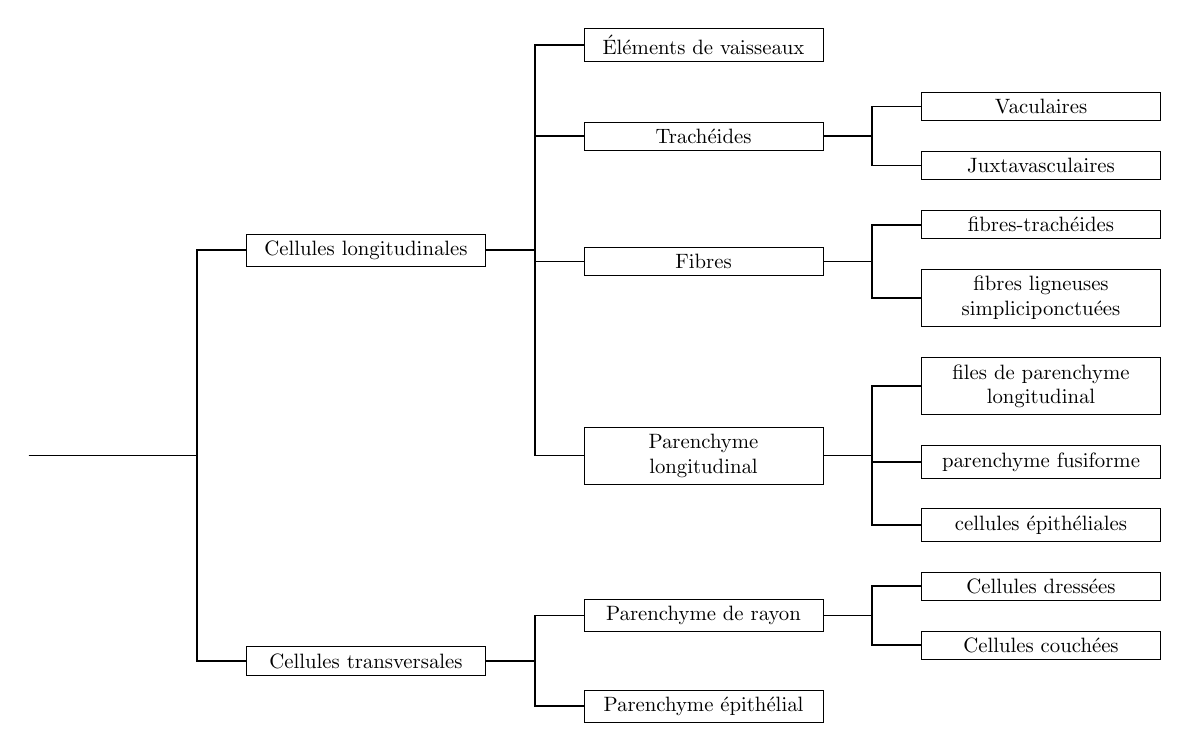
\begin{tikzpicture}[level distance=2.25in,sibling distance=.2in,scale=.75]
\tikzset{edge from parent/.style= 
            {thick, draw,
                edge from parent fork right},every tree node/.style={draw,minimum width=1in,text width=1.5in, align=center},grow'=right}
\Tree 
   [
    [. {Cellules longitudinales}
        [.{Éléments de vaisseaux}
        ]
        [.{Trachéides}
            [.{Vaculaires} ]
            [.{Juxtavasculaires} ]
        ] 
        [. {Fibres}
        	[.{fibres-trachéides} ]
            [.{fibres ligneuses simpliciponctuées} ]
        ]
        [. {Parenchyme longitudinal}
	        [.{files de parenchyme longitudinal} ]
	        [.{parenchyme fusiforme} ]
	        [.{cellules épithéliales} ]
        ] 
    ]
    [. {Cellules transversales}
	    [.{Parenchyme de rayon}
		    [.{Cellules dressées} ]
		    [.{Cellules couchées} ]
	    ] 
	    [.{Parenchyme épithélial}
	    ] 
    ]    
   ]
\end{tikzpicture}
\caption{Les types de cellules orientées dans les directions longitudinale et transversale chez les feuillus}
\label{fig:resum_feuillus}	
\end{figure}


\begin{figure}[h]
\centering
\includegraphics[scale=0.5]{img/ch4_type_cell}
\caption{Forme et longueur relative des principaux types de cellules des bois feuillus (adapté de \cite{hoadley1990identifying})}
\label{fig:ch4_type_cell}
\end{figure}

\begin{figure}[h]
\centering
\includegraphics[scale=0.5]{img/ch4_form_cell_X}
\caption{Forme, diamètre et épaisseur des parois cellulaires relatives des principaux types de cellules des bois feuillus (adapté de \cite{hoadley1990identifying})}
\label{fig:ch4_form_cell_X}
\end{figure}

\section{Cellules orientées longitudinalement}

On peut séparer les cellules orientées longitudinalement en deux grands groupes : les éléments de vaisseaux (trachéides et fibres) et le parenchyme longitudinal.

\begin{description}
\item[Éléments de vaisseaux (trachéides et fibres)] Il s'agit de cellules allongées possédant une variété de types de ponctuations et servant à la conduction de la sève brute et au support mécanique de la tige. Ces cellules perdent leur protoplasme aussitôt qu'elles ont atteint leur maturité à partir des initiales fusiformes du cambium.

\item[Parenchyme longitudinal] Ces cellules conservent leur protoplasme dans l'aubier. Ce sont des cellules courtes possédant des ponctuations simples et servant à l'entreposage des substances nutritives.
\end{description}

\subsection{Éléments de vaisseaux}

Les éléments de vaisseaux sont les unités de base formant les structures composites en forme de tubes que l'on appelle vaisseaux ou pores.  Les éléments de vaisseaux sont les cellules des bois feuillus possédant les plus grands diamètres mais aussi une paroi cellulaire mince.  Ils sont disposés les uns sur les autres en séries verticales et leurs parois terminales sont perforées de façon à former un tube continu permettant le passage des fluides, c'est-à-dire un vaisseau. Les parois terminales sont perforées par action enzymatique avant que le protoplasme ne soit éliminé.  Cette opération produit ce qu'on appelle les cloisons perforées qui ont des formes différentes en fonction des espèces.\\

Les vaisseaux ne sont pas des tubes verticaux rectilignes indépendants les uns des autres. Au contraire, les vaisseaux dévient par rapport à la verticale et ce jusqu'à 30 cm par 5 m de longueur.  De plus, ils sont interconnectés par des ponctuations et cloisons perforées de façon à créer un réseau de pores permettant d'éviter les cul-de-sacs.\\

La longueur des éléments de vaisseaux varie considérablement en fonction des espèces (Tableau~\ref{tab:long_vaiss}) même si peu ou pas de croissance en longueur ne se produit pour ces cellules. Ceci est dû au fait que la longueur des initiales fusiformes du cambium varie d'une espèce à l'autre (0,18 à 1,3 mm).  On remarque que la longueur des éléments de vaisseaux varie d'environ 0,22 à 1,00 mm alors que celle des fibres varie d'environ 0,9 à 1,55 mm pour les principales espèces de feuillus de l'Est de l'Amérique du Nord.\\

Quant au diamètre des vaisseaux ou pores, il est mesuré selon la direction tangentielle et varie de 20 \micro m jusqu'à 300 \micro m en fonction des espèces.

\begin{table}[ht]
	\centering
	\begin{tabular}{l c c c c}
		\hline
		\bf Espèce & \multicolumn{2}{c}{\textbf{Éléments de vaisseaux}} & \multicolumn{2}{c}{\textbf{Fibres}}\\
		& \bf long. moy. (mm) & \bf Écart-type & \bf long. moy. (mm) & \bf Écart-type \\
		\hline
		\hline
		Érable à sucre	&	0,41	&	0,09	&	0,92	&	0,13	\\
		Bouleau jaune	&	0,84	&	0,16	&	1,38	&	0,17	\\
		Bouleau à papier	&	1,00	&	0,26	&	1,35	&	0,15	\\
		Frêne blanc	&	0,29	&	0,03	&	1,26	&	0,17	\\
		Frêne noir	&	0,27	&	0,04	&	1,27	&	0,17	\\
		Noyer cendré	&	0,36	&	0,14	&	1,13	&	0,17	\\
		Noyer noir	&	0,51	&	0,08	&	1,21	&	0,14	\\
		P. faux-tremble	&	0,67	&	0,18	&	1,32	&	0,22	\\
		Chêne rouge	&	0,42	&	0,09	&	1,32	&	0,29	\\
		Orme d’Amérique	&	0,22	&	0,04	&	1,55	&	0,20	\\
		\hline
	\end{tabular}
	\caption{Longueur des éléments de vaisseaux et des fibres des principales espèces de feuillus de l'est de l'Amérique du Nord.}\label{tab:long_vaiss}
\end{table}

\subsubsection{Disposition des vaisseaux}

On peut classer les bois feuillus en trois grands groupes en fonction de la disposition et de la taille des vaisseaux.  Ces critères constituent en fait la première étape dans l'identification des bois feuillus. Ces trois groupes sont illustrés à la figure~\ref{fig:dispo_pores} et décrits ci-dessous.

\begin{description}

\item[Bois à zone poreuse] Les vaisseaux formés au printemps ont un diamètre beaucoup plus grand que ceux formés plus tard en saison. On peut rencontrer une ou plusieurs rangées de gros vaisseaux formant le bois initial.  Les chênes, ormes et frênes sont caractéristiques des bois à zone poreuse.

\item[Bois à zone semi-poreuse] Les vaisseaux formés au printemps ont un diamètre maximum et ce diamètre diminue et demeure constant ou continue à diminuer dans le cerne annuel. Les noyers (\textit{Juglans spp.}) sont caractéristiques des bois à zone semi-poreuse.

\item[Bois à pores diffus] Les vaisseaux ont un diamètre plutôt constant et sont répartis uniformément dans le cerne annuel. Les érables (\textit{Acer spp.}), bouleaux (\textit{Betula spp.}), hêtres (\textit{Fagus spp.}) et tilleuls (\textit{Tilia spp.}) sont caractéristiques des bois à pores diffus.
\end{description}

\begin{figure}[h]
\centering
\includegraphics[scale=0.6]{img/ch4_dispositon_pores}
\caption{Disposition des pores chez les feuillus. Image préparée par Julie Ferland pour \cite{achim2010dendroecologie}.}
\label{fig:dispo_pores}
\end{figure}

\subsubsection{Caractéristiques des éléments de vaisseaux}

Certaines caractéristiques des éléments de vaisseaux sont utilisées pour l'identification des bois feuillus.  Il s'agit 1) de la forme des cloisons perforées, 2) de la disposition des ponctuations intervasculaires et 3) de la présence d'épaississements spiralés.

\subsubsection{Forme des cloisons perforées}\label{cloisons}

Les cloisons perforées sont les ouvertures que l'on retrouve dans la paroi commune entre deux éléments de vaisseaux.  On retrouve habituellement deux cloisons perforées par élément de vaisseau mais il peut y en avoir davantage pour permettre l'interconnexion entre les vaisseaux. On trouve plusieurs types de cloisons perforées:

\begin{description}
\item[Perforation unique (\textit{simple})] La perforation unique consiste en une ouverture simple occupant habituellement toute la surface de la cloison perforée (Figure~\ref{fig:cloisons}). On retrouve ce type de perforation chez environ 80\% des feuillus d'Amérique du Nord. On nomme bourrelet de la perforation le résidu de la paroi cellulaire perforée qui forme un anneau autour d'une perforation unique.

\begin{figure}[h]
	\centering
	\includegraphics[scale=0.6]{img/ch4_perforation_cloison}
	\caption{Cloisons perforées chez les éléments de vaisseaux.  a) perforation unique; b) perforation en grille; c) perforation en réseau. Image préparée par Julie Ferland pour \cite{achim2010dendroecologie}.}
	\label{fig:cloisons}
\end{figure}

\item[Perforation en grille (\textit{scalariform})] La perforation en grille consiste en une série d'ouvertures parallèles orientées transversalement (Figure~\ref{fig:cloisons}). Les résidus de la paroi cellulaire demeurant dans la cloison perforée ont l'apparence des barreaux d'une échelle (Figure~\ref{fig:grille}) d'où le nom anglais \og scalariform \fg. Elles sont typiques chez les bouleaux (\textit{Betula spp.}). Le nombre de barreaux varie d'une espèce à l'autre.  On peut retrouver les deux types de perforation, unique et en grille, chez certaines espèces (ex. : hêtre à grandes feuilles (\textit{Fagus grandifolia})).

\item[Perforation en réseau (\textit{reticulate})] La perforation en réseau est semblable à la perforation en grille sauf que les résidus de la paroi cellulaire encore présents dans la cloison perforée ont l'apparence d'un filet plutôt irrégulier (Figures~\ref{fig:cloisons}~et~\ref{fig:reseau}). Ce type de perforation n'est toutefois pas présent chez les espèces commerciales de l'Amérique du Nord.
\end{description}

\begin{figure}[h]
\centering
\includegraphics[scale=1]{img/ch4_grille}
\caption{Perforation en grille chez Alnus glutinosa (d'après \cite{butterfield2012three})}
\label{fig:grille}
\end{figure}

\begin{figure}[h]
\centering
\includegraphics[scale=1]{img/ch4_reseau}
\caption{Perforation en réseau chez \textit{Coprosma tenuicaulis} (d'après \cite{butterfield2012three})}
\label{fig:reseau}
\end{figure}

\subsubsection{Disposition des ponctuations intervasculaires}\label{disposition}

Tout comme c'est le cas chez les résineux, le type de ponctuations que l'on retrouve entre les cellules des bois feuillus dépend du type de cellules en contact entre elles.  Il faut noter en particulier que les parois des cellules de parenchyme des feuillus sont plus épaisses que celles des résineux. Il s'agit de parois primaires \og épaissies \fg pouvant donner des couples de ponctuations aréolées ou semi-aréolées. Il faut remarquer que chez les feuillus, les couples de ponctuations aréolées ne comportent pas de torus comme chez les conifères.\\

On peut donc avoir les types de ponctuation suivants en fonction du type de cellules en cause (Figure~\ref{fig:type_ponct_feuillus}).

\begin{figure}[h]
	\centering
	
	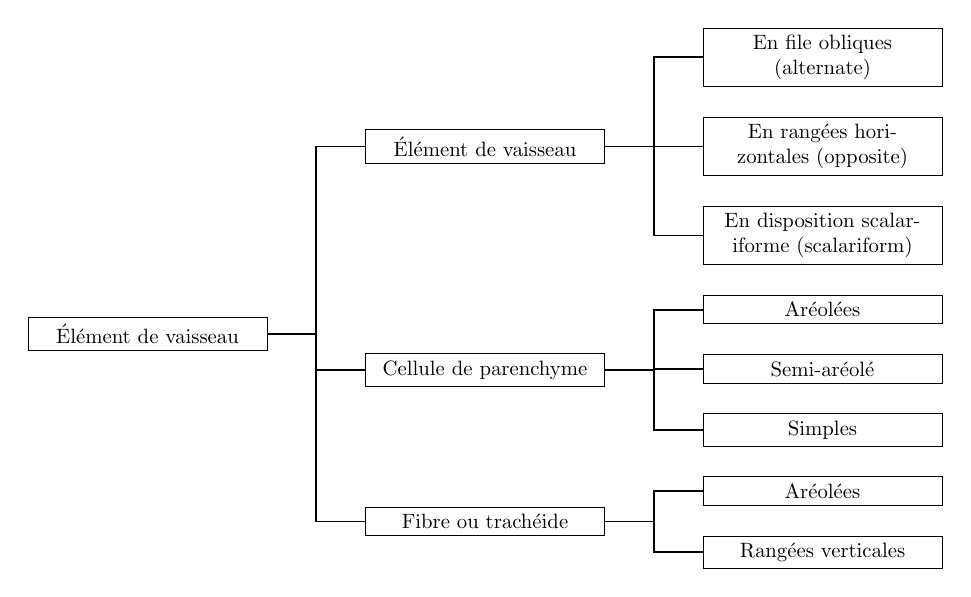
\begin{tikzpicture}[level distance=2.25in,sibling distance=.2in,scale=.75]
	\tikzset{edge from parent/.style= 
		{thick, draw,
			edge from parent fork right},every tree node/.style={draw,minimum width=1in,text width=1.5in, align=center},grow'=right}
	\Tree 
	[. {Élément de vaisseau}
		[.{Élément de vaisseau}
			[.{En file obliques (alternate)} ]
			[.{En rangées horizontales (opposite)} ]
			[.{En disposition scalariforme (scalariform)} ]
		]
		[.{Cellule de parenchyme}
			[.{Aréolées} ]
			[.{Semi-aréolé} ]
			[.{Simples} ]
		] 
		[. {Fibre ou trachéide}
			[.{Aréolées} ]
			[.{Rangées verticales} ]
		] 
	]
	\end{tikzpicture}
	\caption{Types de ponctuations entre les éléments de vaisseaux et chacun des types de cellules du bois des feuillus}
\label{fig:type_ponct_feuillus}	
\end{figure}

Les ponctuations intervasculaires sont celles que l'on retrouve sur les parois des éléments de vaisseaux, particulièrement en plan longitudinal-tangentiel. Elles servent au passage de la sève brute d'un vaisseau à l'autre. Il s'agit de couples de ponctuations aréolées.  On reconnaît trois types de disposition des ponctuations intervasculaires : 1) les ponctuations intervasculaires en files obliques, 2) les ponctuations intervasculaires en rangées horizontales et 3) les ponctuations intervasculaires en disposition scalariforme. Les trois types sont illustrés à la Figure~\ref{fig:intervasc}.


\begin{figure}[h]
\centering
\includegraphics[scale=0.55]{img/ch4_ponctuations_intervasculaires}
\caption{Disposition des ponctuations intervasculaires. Image préparée par Julie Ferland pour \cite{achim2010dendroecologie}.}
\label{fig:intervasc}
\end{figure}	

Les ponctuations intervasculaires peuvent être classées selon leur dimension:

\begin{itemize}
\item diamètre de 2 à 4 \micro m:	petites (\textit{Betula spp.})
\item diamètre de 5 à 10 \micro m:	moyennes (\textit{Acer spp.})
\item diamètre de 12 à 50 \micro m:	grandes (\textit{Magnolia spp.})
\end{itemize}

\subsubsection{Épaississements spiralés dans les éléments de vaisseaux}\label{epais}

Des épaississements peuvent être présents dans la paroi secondaire des éléments de vaisseaux, des fibres et des trachéides chez certaines espèces et ils servent de critère d'identification. Ils sont des épaississements de la couche \hyperref[s3]{S\sub{3}} de la paroi cellulaire (voir chapitre~\ref{paroi}). Chez les bois à pores diffus, lorsque les épaississements spiralés sont présents, ils le sont pour tous les vaisseaux du cerne annuel. Chez les bois à zone poreuse, lorsqu'ils sont présents, on ne retrouve les épaississements spiralés  que chez les plus petits vaisseaux du bois final (Figure~\ref{vaiss_spiral}). Les épaississements spiralés dans les vaisseaux sont caractéristiques des érables (\textit{Acer spp.}), du cerisier tardif (\textit{Prunus serotina}) et du tilleul d'Amérique (\textit{Tilia americana}). On retrouve des épaississements spiralés dans les trachéides vasculaires chez l'orme rouge (\textit{Ulmus rubra}).

\begin{figure}[h]
\centering
\includegraphics[scale=0.8]{img/ch4_vaiss_spiral}
\caption{Épaississements spiralés dans un vaisseau de tilleul d'Amérique (\textit{Tilia americana}) (grossissement $\times$400).}
\label{vaiss_spiral}
\end{figure}

\subsubsection{Incrustations dans les éléments de vaisseaux}

Un thylle (tylosis) est une excroissance d'un parenchyme adjacent dans un vaisseau, à travers une ponctuation. Les thylles peuvent obstruer un vaisseau ou le bloquer complètement si ils sont suffisamment nombreux. Les thylles sont généralement formés dans la partie intérieure de l'aubier, juste avant que la duraminisation se produise.  Ils peuvent parfois se former au début de l'aubier s'il y a sécheresse, blessure ou infection. On parle alors de thylles traumatiques. Le chêne blanc (\textit{Quercus alba}) est une espèce caractéristique présentant de nombreux thylles. Des thylles caractéristiques sont présentés à la Figure~\ref{fig:thylles}. \\

\begin{figure}[h]
	\centering
	\includegraphics[scale=0.6]{img/ch4_thylles}
	\caption{Thylles dans les vaisseaux du chêne blanc (\textit{Quercus alba}) (à gauche) et de l'acacia blanc (Robinia pseudoacacia) (à droite) (grossissement: $\times$20) (d'après \cite{hoadley1990identifying})}
\label{fig:thylles}
\end{figure}

Des gommes et des résines peuvent aussi être sécrétées dans les vaisseaux.  Ces substances proviennent souvent des parenchymes de rayon et s'écoulent dans les vaisseaux par les ponctuations que l'on retrouve entre les vaisseaux et les parenchymes de rayon.  Elles sont caractéristiques de quelques espèces d'Amérique du Nord, par exemple le cerisier tardif (\textit{Prunus serotina}).

\subsubsection{Volume des vaisseaux}

Les vaisseaux constituent en moyenne 30\% du volume des bois feuillus, mais avec une variabilité importante entre les espèces (de 7 à 55\%). Chez les bois feuillus d'Amérique du Nord, la moyenne est plutôt d'environ 20\% du volume. La proportion du volume du bois occupée par les diverses composantes est présentée au Tableau~\ref{tab:prop_feuillus}.

\begin{table}[ht]
\centering
	\begin{tabular}{l c c c c}
	\hline
		& \bf Vaisseaux	& \bf	Fibres	& \bf	Rayons	& \bf	Parenchyme longitudinal	\\
		\hline
		\hline
		Érable à sucre	&	21,0	&	61,0	&	17,9	&	0,1	\\
		Bouleau jaune	&	21,4	&	63,8	&	10,8	&	2,0	\\
		Bouleau à papier	&	10,6	&	75,7	&	11,7	&	2,0	\\
		Cerisier tardif	&	41,4	&	41,4	&	17,2	&	-	\\
		Frêne blanc	&	20,4	&	61,7	&	11,9	&	4,2	\\
		Frêne noir	&	11,6	&	69,4	&	12,0	&	7,0	\\
		Noyer cendré	&	22,6	&	58,0	&	10,4	&	9,0	\\
		Noyer noir	&	21,0	&	48,7	&	16,8	&	13,5	\\
		Chêne rouge	&	21,6	&	43,5	&	21,4	&	13,5	\\
		Orme d’Amérique	&	48,0	&	34,7	&	11,3	&	6,0	\\
	\hline
	\end{tabular}
\caption{Proportion (\%) du volume du bois occupé par ses diverses composantes.}
\label{tab:prop_feuillus}
\end{table}

\subsection{Trachéides}

\subsubsection{Trachéides vasculaires}

Les trachéides vasculaires ressemblent aux vaisseaux du bois final mais elles ne possèdent pas de cloison perforée dans les bouts (éléments de vaisseaux imparfaits). Elles sont associées à des vaisseaux, elles sont organisées en séries verticales (longitudinales) et possèdent des couples de ponctuations aréolées.  Elles peuvent avoir des épaississements spiralés et ont l'apparence de petits vaisseaux en coupe transversale.  Les trachéides vasculaires sont présentes chez les ormes (\textit{Ulmus spp.}) au voisinage des vaisseaux du bois final.

\subsubsection{Trachéides juxtavasculaires}

Les trachéides juxtavasculaires sont de courtes trachéides de forme irrégulière, se trouvant à proximité immédiate des vaisseaux et ne faisant pas partie d'une série axiale définie. Elles ne possèdent pas de cloison perforée dans les bouts mais possèdent un nombre important de couples de ponctuations aréolées et des parois minces. On les retrouve surtout autour des vaisseaux du bois initial et elles forment des zones irrégulières en forme de flammes en coupe longitudinale-radiale. On les retrouve, entre autres, chez les chênes (\textit{Quercus spp.}) et les frênes (\textit{Fraxinus spp.}).

\subsection{Fibres}

Les fibres sont de longues cellules de faible diamètre, possédant des parois cellulaires épaisses mais ne possédant pas de cloison perforée dans les bouts. On distingue deux types de fibres : les fibres-trachéides et les fibres ligneuses simpliciponctuées.

\subsubsection{Fibres-trachéides}

Les fibres-trachéides possèdent de nombreux couples de ponctuations aréolées habituellement faciles à observer au microscope optique.

\subsubsection{Fibres ligneuses simpliciponctuées}

Les fibres ligneuses simpliciponctuées  possèdent des ponctuations simples habituellement peu nombreuses ayant l'apparence de petites ouvertures circulaires souvent difficiles à voir au microscope optique. On peut retrouver un type de fibre ou l'autre ou bien les deux chez une espèce en particulier. Il est souvent difficile d'identifier le type de fibre avec certitude. \\

La proportion du volume total du bois occupé par les fibres-trachéides et les fibres ligneuses simpliciponctuées varie de 25\% à 75\% en fonction des espèces et en détermine largement la résistance mécanique.

\subsection{Parenchyme longitudinal}

Le parenchyme longitudinal est constitué de cellules courtes en forme de briques disposées en files longitudinales. Les cellules de parenchyme gardent longtemps leur protoplasme et restent physiologiquement actives. Leur rôle essentiel est la mise en réserve et la distribution de substances nutritives (hydrates de carbone). Pour cela, leur paroi est peu lignifiée et abondamment ponctuée. Leur activité cesse dans le bois de duramen. Ces cellules de parenchyme sont connectées entre elles par des ponctuations simples.\\

Chez les feuillus, le parenchyme longitudinal est disposé de façon particulière en fonction des espèces. Cette disposition caractéristique est utilisée comme critère d'identification. Le parenchyme longitudinal peut occuper une proportion importante du volume du bois en fonction des espèces. Cette proportion varie d'environ 1 à 25\% chez les espèces nord-américaines et peut aller jusqu'à 50\% chez certains feuillus tropicaux.\\

On reconnaît trois types de parenchyme longitudinal : 1) les files de cellules de parenchyme longitudinal, 2) les cellules de parenchyme fusiforme et 3) les cellules de parenchyme épithélial. Nous verrons chaque type dans les paragraphes qui suivent.

\subsubsection{Files de cellules de parenchyme longitudinal}

Les files de cellules de parenchyme longitudinal sont formées par divisions transversales de l'initiale fusiforme fille.  Elles consistent en des groupements de cellules pouvant varier de une à plusieurs et sont souvent visibles en coupe transversale. Leurs arrangements variables peuvent être utilisés pour l'identification. Classement du parenchyme longitudinal :

\begin{description}

\item[Parenchyme apotrachéal] Le parenchyme apotrachéal est typiquement isolé des vaisseaux. Le parenchyme apotrachéal peut être :

\begin{description}
	\item[dispersé] Le parenchyme apotrachéal dispersé est caractérisé par des cellules de parenchyme isolées en plan RT tel qu'illustré à la Figure~\ref{fig:parenchymes_feuillus}A.  Il est caractéristique des érables (\textit{Acer spp.}).
	
	\item[dispersé en chaînettes] Le parenchyme apotrachéal dispersé en chaînettes est caractérisé par des cellules de parenchyme regroupées en de courtes lignes tangentielles disposées entre les rayons en plan RT tel qu'illustré à la Figure~\ref{fig:parenchymes_feuillus}B.  Il est caractéristique des noyers (\textit{Juglans spp.}) et des tilleuls (\textit{Tilia spp.}).
	arenchyme apotrachéal terminal (ou marginal)

	\item[terminal] Le parenchyme apotrachéal est caractérisé par des cellules de parenchyme regroupées en couches plus ou moins larges à la fin du cerne annuel en plan RT tel qu’illustré à la Figure~\ref{fig:parenchymes_feuillus}C. Il est caractéristique des peupliers (\textit{Populus spp.}).
	
	\item[en couches] Le parenchyme apotrachéal en couches est caractérisé par des cellules de parenchyme regroupées en couches plus ou moins larges qui ne sont pas nécessairement localisées à la fin du cerne annuel en plan RT tel qu'illustré à la Figure~\ref{fig:parenchymes_feuillus}D. Il est caractéristique des caryers (\textit{Carya spp.}).
\end{description}

\item[Parenchyme paratrachéal] Le parenchyme paratrachéal est typiquement associé aux vaisseaux ou aux trachéides vasculaires. Il peut être :

\begin{description}
	\item[juxtavasculaire] Le parenchyme paratrachéal juxtavasculaire est caractérisé par quelques cellules de parenchyme disposées autour des vaisseaux mais ne les entourant pas complètement en plan RT tel qu'illustré à la Figure~\ref{fig:parenchymes_feuillus}E.  Il est caractéristique des érables (\textit{Acer spp.}).
	
	\item[circumvasculaire] Le parenchyme paratrachéal circumvasculaire est caractérisé par une ou plusieurs couches de cellules de parenchyme disposées autour des vaisseaux et les entourant complètement en plan RT tel qu'illustré à la Figure~\ref{fig:parenchymes_feuillus}F.  Il est caractéristique des frênes (\textit{Fraxinus spp.}).

	\item[aliforme] Le parenchyme paratrachéal aliforme est caractérisé par une ou plusieurs couches de cellules de parenchyme disposées autour des vaisseaux, les entourant complètement et s'étendant de chaque côté en forme d'aile en plan RT tel qu'illustré à la Figure~\ref{fig:parenchymes_feuillus}G. Il est caractéristique des frênes (\textit{Fraxinus spp.}).
	
	\item[anastomosé (confluent)] Le parenchyme paratrachéal anastomosé est caractérisé par une ou plusieurs couches de cellules de parenchyme disposées autour de plusieurs vaisseaux, les entourant complètement et formant des bandes irrégulières tangentielles en plan RT tel qu'illustré à la Figure~\ref{fig:parenchymes_feuillus}H. Il est caractéristique du \textit{Robinia pseudoacacia}.
	
	\item[en couche] Le parenchyme paratrachéal en couche est caractérisé par une ou plusieurs couches de cellules de parenchyme disposées autour de plusieurs vaisseaux, les entourant complètement et formant de larges bandes irrégulières tangentielles en plan RT tel qu'illustré à la Figure~\ref{fig:parenchymes_feuillus}I.  Il est caractéristique des caryers (\textit{Carya spp.}) et des hêtres (\textit{Fagus spp.}).
	
	\marginpar{Des parenchymes apotrachéals et paratrachéals peuvent être présents tous les deux chez la même espèce.}	
\end{description}

\end{description}

\begin{figure}[h]
\centering
\includegraphics[scale=0.75]{img/ch4_parenchymes}
\caption{Différents types de parenchymes -- A. Dispersé B. Dispersé en chaînette C. Terminal D. En couche E. Juxtavasculaire F. Circumvasculaire G. Aliforme H. Anastomosé I. En couche}
\label{fig:parenchymes_feuillus}
\end{figure}

\subsubsection{Cellules de parenchyme fusiformes}

Le parenchyme fusiforme est un parenchyme longitudinal dérivé d'une initiale fusiforme sans subdivision.  Il s'agit donc d'une cellule de parenchyme allongée.  Ce type de parenchyme est rare chez les bois nord-américains.

\subsubsection{Cellules de parenchyme épithélial}

Les cellules de parenchyme épithélial tapissent les cavités des canaux longitudinaux (gomme ou résine) présents chez certains feuillus tropicaux.  Ces canaux sont absents chez les feuillus nord-américains.


\section{Cellules transversales}

Les cellules transversales constituent essentiellement les rayons comme c'est le cas chez les résineux. Les rayons présentent toutefois une plus grande variabilité chez les feuillus que chez les résineux à l'égard de la forme, de l'arrangement, de la largeur et de la hauteur.


\subsection{Composition des rayons}

Chez les feuillus, les rayons sont composés uniquement de cellules de parenchyme. Ces cellules sont de deux types: les cellules dressées et les cellules couchées. Les cellules dressées sont des cellules allongées verticalement et les cellules couchées sont des cellules allongées horizontalement.\\

On classe les rayons en deux catégories, les rayons homogènes et les rayons hétérogènes uniquement. Les rayons hétérogènes sont composés de cellules couchées et de cellules dressées (Figure~\ref{fig:rayons_feuillus}). Les rayons homogènes sont composés de cellules couchées ou de cellules dressées.

\begin{figure}[h]
\centering
\includegraphics[scale=0.75]{img/ch4_rayons}
\caption{Différents types de rayons chez les feuillus (adapté de \cite{jane1970structure}).}
\label{fig:rayons_feuillus}
\end{figure}

\subsection{Taille des rayons}

Chez les feuillus, les rayons sont visibles ou non à l'oeil nu. Les peupliers (\textit{Populus spp.}) possèdent des rayons unisériés mais la plupart du temps, les rayons des feuillus sont plurisériés et ils peuvent être très larges comme chez les chênes (\textit{Quercus spp.}) où ils atteignent jusqu'à 30 cellules de large (30-sériés). Chez certaines espèces, les rayons sont de deux dimensions distinctes, soit des rayons unisériés et des rayons plurisériés. C'est le cas de l'érable à sucre (\textit{Acer saccharum}) et du hêtre à grandes feuilles (\textit{Fagus grandifolia}). La hauteur des rayons varie d'environ 20 m (une cellule) jusqu'à 50 mm.

\subsection{Espacement des rayons}

L'espacement des rayons est défini comme le nombre de rayons par millimètre en section transversale. Pour le déterminer, on mesure le nombre de rayons par mm traversant la fin ou le début du cerne annuel. Le classement de l'espacement des rayons est donné au Tableau~\ref{tab:espace_rayons}.

\begin{table}[ht]
	\centering
	\begin{tabular}{l l}
		\hline
		\bf Rayon/mm & \bf Espacement\\
		\hline
		\hline
		5 ou moins & Largement espacés\\
		6 à 9 & Normalement espacés \\
		10 à 13 & Plutôt rapprochés \\
		14 à 20 & Rapprochés \\
		21 ou plus & Extrêmement rapprochés\\
		\hline	
	\end{tabular}
	\caption{Classement de l'espacement des rayons}
\label{tab:espace_rayons}
\end{table}

\subsection{Ponctuations dans les rayons}

Les ponctuations des parenchymes de rayon vont de simples et petites à aréolées et grandes en fonction des cellules en contact avec les parenchymes de rayon. On reconnaît trois principaux types de ponctuations rayon-vaisseau:

\begin{enumerate}
\item Ponctuations rayon-vaisseau simples et allongées.
\item Ponctuations rayon-vaisseau simples à aréolées et variables en forme et en dimension.
\item Ponctuations rayon-vaisseau semblables aux ponctuations intervasculaires.
\end{enumerate}

\subsection{Contenus cellulaires}

Des contenus cellulaires sont souvent présents dans les cellules des rayons.  Il s'agit de cristaux, de silice, de substances amorphes (gommes, résines, tannins, huiles, latex, \ldots) ou d'amidon.

\subsection{Proportion des rayons}

La proportion du volume des bois feuillus constituée par des rayons varie de 10 à 20\%. La proportion en volume des rayons a un effet important sur les propriétés mécaniques du bois en termes de stabilité dimensionnelle, de formation de gerces et de fentes internes lors du séchage, de perméabilité et de résistance mécanique.

\subsection{Canaux à gomme}

Des canaux à gommes normaux ou traumatiques peuvent être présents. Ces canaux contiennent des cellules épithéliales sécrétant des gommes ou résines. Des canaux à gommes \og normaux \fg ne sont pas présents chez les espèces nord-américaines.

\section{L'anatomie du bois des feuillus en un clin d'œil}

La figure~\ref{fig:Fahn_feu} illustre l'organisation des différentes cellules du bois des résineux.

\begin{figure}[h]
\centering
\includegraphics[scale=0.7]{img/ch4_Fahn_feu}
\caption{Structure tridimensionnelle générale des feuillus (adapté de \cite{fahn1990plant})}
\label{fig:Fahn_feu}
\end{figure}
%
%
%
%Références
%
%
%
%Butterfield, B.G.; Meylan, B.A. 1980. Three-dimensional structure of wood. An ultrastructural approach. Second edition. Chapman and Hall, London, New York. 103 p.
%
%Fahn, A. 1990. Plant anatomy. Fourth edition. Pergamon Press, Oxford. 588 p.
%
%Hoadley, R.B. 1990. Identifying wood. Accurate results with simple tools. The Taunton Press Inc. Connecticut, USA. 223 p.
%
%Jane, F.W. 1970. The structure of wood.  Second Edition.  Adam and Charles Black, London.  478 p.
%
%Panshin, A.J.; de Zeeuw, C. 1980. Textbook of wood technology. Fourth edition. McGraw-Hill Book Co. New York. 722 p.
%

% apr lecture c'est quqnd même très très superficiel comme chapitre non ?


\chapter{Croissance en hauteur et en diamètre}

\begin{abstract}
Ce chapitre décrit comment l'activité des méristèmes est responsable de la croissance en hauteur et diamètre des arbres. Nous nous attarderons surtout à l'action du cambium, ou méristème secondaire, dont l'importance est fondamentale en sciences du bois. Il s'agit d'une fine couche de cellules dont la division est responsable de la formation des cellules de xylème et de phloème. La fin du chapitre montre comment l'action du cambium a une importance fondamentale sur la variabilité de la longueur des trachéides ou des fibres du centre de la tige vers l'écorce. Ces patrons de variabilité seront traités en détails dans les chapitres suivants. 
\end{abstract}

\minitoc

\section{Introduction}

La croissance des plantes ligneuses se produit selon deux mécanismes distincts, soit la croissance en hauteur et la croissance en diamètre. Chacun de ces mécanismes de croissance est assuré par des tissus particuliers appelés \textbf{méristèmes}. Les méristèmes sont des tissus embryonnaires \textbf{peu différenciés} et en constante division cellulaire. Ils produisent donc constamment de nouveaux tissus s'ajoutant à la plante.\\

On reconnait deux types de méristèmes dans les plantes ligneuses. Premièrement le \textbf{méristème apical} (ou méristème primaire) responsable de la croissance en hauteur et situé au bout des branches. Deuxièmement, \textbf{le cambium} (ou méristème secondaire) responsable de la croissance en diamètre et situé entre le xylème et le phloème.

\section{Méristème apical}

Le méristème apical est responsable de la croissance primaire, c'est-à-dire de l'élongation de la pousse terminale de la tige et des branches. Il produit trois types de tissus, le protoderme (ou épiderme), le procambium et le méristème de la moelle. Ces tissus évoluent vers le protoderme, le phloème secondaire, le cambium et le xylème secondaire. La Figure~\ref{fig:apical} montre chacune des étapes entre les deux. Comme l'objet de ce cours est d'abord relié à la croissance secondaire, vous pouvez vous contenter de retenir le rôle principal de ce méristème (vous n'avez pas à retenir chacune des étapes présentées à la Figure~\ref{fig:apical})

\begin{figure}[h]
	\centering
	\includegraphics[scale=0.3]{img/ch5_apical}
	\caption{Représentation schématique du méristème apical (adapté de \cite{bowyer2007forest}).}
	\label{fig:apical}
\end{figure}.

\section{Cambium (méristème secondaire)}

Le cambium est une couche de cellules méristématiques en voie de division active située entre le xylème et le phloème (Figure~\ref{fig:camb_xyl}). Ces cellules sont appelées initiales du cambium. On retrouve deux types d'initiales du cambium, les \textbf{initiales fusiformes} et les \textbf{initiales de rayon}.

\begin{figure}[h]
	\centering
	\includegraphics[scale=0.7]{img/ch5_camb_xyl}
	\caption{Représentation schématique du cambium, des initiales fusiformes et des initiales de rayon (adapté de \cite{bowyer2007forest}).}
\label{fig:camb_xyl}
\end{figure}

\subsection{Initiales fusiformes}

Les initiales fusiformes donnent naissance aux cellules longitudinales autant du côté du xylème que du phloème. En plan LT, les initiales fusiformes ont une forme aplatie et effilée (Figure~\ref{fig:camb_xyl}) alors qu'elles ont un profil en fuseau dans le plan LR (Figure~\ref{fig:periclinal}). Elles sont d'une longueur variant de 2 à 9 mm et d'un diamètre de 30 µm et plus chez les résineux. Chez les feuillus, les initiales fusiformes ont une longueur variant de 0,3 à 2 mm.\\

Le cambium étagé est un cas particulier que l'on rencontre chez certaines espèces incluant l'acacia blanc (\textit{Robinia pseudoacacia}). Chez ces bois, les initiales fusiformes sont de longueur plus ou moins uniforme et sont groupées en rangées horizontales (Figure~\ref{fig:cambium_etage}).  La longueur des initiales fusiformes chez les bois à cambium étagé varie de 140 µm à 520 µm.

\begin{figure}[h]
	\centering
	\includegraphics[scale=0.5]{img/ch5_periclinal}
	\caption{Cloisonnement périclinal des initiales fusiformes du cambium (adapté de \cite{bowyer2007forest}).}
	\label{fig:periclinal}
\end{figure}

\begin{figure}[h]
	\centering
	\includegraphics[scale=0.4]{img/ch5_cambium_etage}
	\caption{Cambium en plan LT.  1) cambium étagé, 2) cambium non-étagé (adapté de \cite{fahn1990plant}).}
\label{fig:cambium_etage}
\end{figure}

\subsection{Initiales de rayon}

Les initiales de rayon sont des cellules de forme cubique donnant naissance aux cellules de rayon et aux cellules épithéliales (Figures~\ref{fig:cambium_etage}~et~\ref{fig:cellules_resume}). La Figure~\ref{fig:cellules_resume} peut vous servir de résumé des chapitres sur l'anatomie du bois des \hyperref[resineux]{résineux} et des \hyperref[feuillus]{feuillus}.

\subsubsection{Processus de division cellulaire dans le cambium}

Les cellules du cambium peuvent se diviser successivement pour former de nouvelles initiales du cambium et de nouvelles cellules de xylème et de phloème.  Les initiales du cambium se divisent selon deux mécanismes différents : 1) selon un cloisonnement \textbf{périclinal} et 2) selon un cloisonnement \textbf{anticlinal}.

\begin{figure}[h]
\centering
\includegraphics[width=1\textwidth]{img/ch5_cellules_resume}
\caption{Types de cellules du xylème produites par les initiales du cambium chez les résineux et les feuillus (adapté de \cite{jane1970structure}).}
\label{fig:cellules_resume}
\end{figure}

\subsubsection{Cloisonnement périclinal}

Le cloisonnement périclinal s'effectue selon un plan LT tel qu'illustré aux Figures~\ref{fig:periclinal}, \ref{fig:peri_anti} et \ref{fig:peri_anti_haut}. Ce type de cloisonnement permet la croissance en diamètre de la tige par la formation de nouvelles cellules de xylème et de phloème.

\begin{figure}[h]
\centering
\includegraphics[scale=0.8]{img/ch5_peri_anti}
\caption{Cloisonnement périclinal et anticlinal d'une initiale fusiforme du cambium (d'après \cite{doucet2009manuel}).}
\label{fig:peri_anti}
\end{figure}

\begin{figure}[h]
\centering
\includegraphics[scale=0.5]{img/ch5_peri_anti_haut}
\caption{Cloisonnement périclinal et anticlinal d'une initiale du cambium (adapté de \cite{bowyer2007forest}).}
\label{fig:peri_anti_haut}
\end{figure}

\subsubsection{Cloisonnement anticlinal}

Le cloisonnement anticlinal s'effectue selon un plan LR tel qu'illustré aux Figures~\ref{fig:peri_anti} et \ref{fig:peri_anti_haut}. Il est responsable de la formation de nouvelles cellules du cambium permettant la croissance en circonférence de ce dernier. Il faut remarquer que la croissance en circonférence du cambium est également due à la croissance subséquente des initiales du cambium en hauteur et en diamètre suite à la division cellulaire tel qu'illustré à la Figure~\ref{fig:elongation}.\\

La production de nouvelles initiales de rayon a lieu selon différents mécanismes.  Elles peuvent être produites par la réduction en longueur d'un certain nombre d'initiales fusiformes ou par la division cellulaire d'initiales fusiformes ou de parties d'initiales fusiformes tel qu'illustré à la Figure~\ref{fig:init_rayons}. Dans le cas des feuillus à rayons plurisériés, le nombre d'initiales de rayons augmente par division des initiales de rayon présentes ou par fusion de plusieurs rayons voisins.\\

\begin{figure}[h]
\centering
\includegraphics[scale=0.7]{img/ch5_elongation}
\caption{Cloisonnement anticlinal et allongement des initiales fusiformes du cambium. A) l'initiale se divise selon un cloisonnement anticlinal, B) et C) les deux cellules ainsi produites s'allongent (d'après \cite{jane1970structure}).}
\label{fig:elongation}
\end{figure}

\begin{figure}[h]
\centering
\includegraphics[scale=0.7]{img/ch5_init_rayons}
\caption{Formation des initiales de rayon à partir des initiales fusiformes (d'après \cite{panshin1980textbook}).}
\label{fig:init_rayons}
\end{figure}

\subsection{Mécanisme de formation des cellules de xylème et de phloème}

La croissance de l'arbre en diamètre est causée par le cloisonnement périclinal des initiales fusiformes et des initiales de rayon. Ces cloisonnements peuvent produire soit une nouvelle initiale de cambium et une cellule-mère de xylème, soit une nouvelle initiale de cambium et une cellule-mère de phloème. Les cellules-mères de xylème sont produites plus fréquemment que les cellules-mères de phloème. Une cellule-mère de phloème se divisera en deux cellules de phloème alors qu'une cellule-mère de xylème se divisera en deux cellules-filles de xylème qui se diviseront à nouveau chacune en deux cellules de xylème. On obtient comme résultat qu'une division par cloisonnement périclinal de l'initiale de cambium résulte en deux nouvelles cellules de phloème ou quatre nouvelles cellules de xylème.  De plus, un moins grand nombre de divisions de l'initiale de cambium donnent naissance à une cellule-mère de phloème. Ceci explique que le cambium produit beaucoup plus de cellules de xylème que de phloème. Le mécanisme général de formation des cellules de xylème et de phloème est présenté aux Figures~\ref{fig:xyl_phlo} et \ref{fig:xyl_phlo_img}.

\subsection{Variation de la longueur des initiales fusiformes du cambium}

La longueur des initiales fusiformes du cambium varie en fonction d'un certain nombre de facteurs. En règle générale, la longueur des initiales fusiformes détermine la longueur des cellules du xylème et du phloème.  De plus, la longueur des initiales fusiformes est inversement proportionnelle au taux de cloisonnement anticlinal. Ceci implique que plus le taux de croissance est élevé, plus les initiales fusiformes sont courtes.

\begin{figure}[h]
\centering

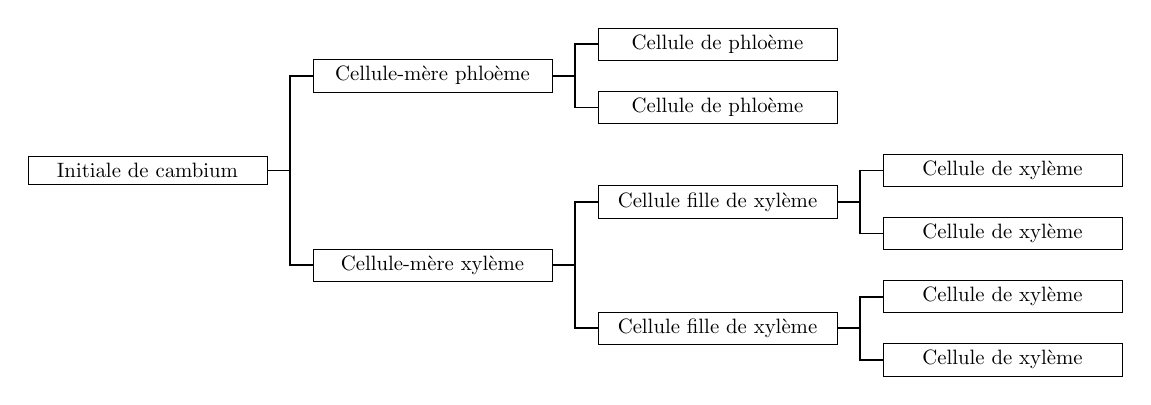
\begin{tikzpicture}[level distance=1.9in,sibling distance=.2in,scale=.75]
\tikzset{edge from parent/.style= 
            {thick, draw,
                edge from parent fork right},every tree node/.style={draw,minimum width=1in,text width=1.5in, align=center},grow'=right}
\Tree 
    [. {Initiale de cambium}
        [.{Cellule-mère phloème}
            [.{Cellule de phloème} ]
            [.{Cellule de phloème} ]
        ]
        [.{Cellule-mère xylème}
            [.{Cellule fille de xylème} 
            	[. {Cellule de xylème} ] 
            	[. {Cellule de xylème} ] ]
            [.{Cellule fille de xylème} 
                 [. {Cellule de xylème} ] 
                 [. {Cellule de xylème} ] ]
        ] 
    ]
\end{tikzpicture}
\caption{Mécanisme de formation des cellules de xylème et de phloème}
\label{fig:xyl_phlo}	
\end{figure}


\begin{figure}[h]
\centering
\includegraphics[scale=0.8]{img/ch5_develop_cambium}
\caption{Mécanisme de formation des cellules de xylème et de phloème (adapté de \cite{panshin1980textbook}).}
\label{fig:xyl_phlo_img}
\end{figure}
%
%
\subsubsection{Effet de la distance radiale de la moelle vers l'écorce}

La longueur des initiales fusiformes augmente de la moelle vers l'écorce comme le montre la Figure~\ref{fig:cloisonnement_long}. De plus, la proportion des initiales fusiformes subissant un cloisonnement anticlinal diminue de la moelle vers l'écorce.

\subsubsection{Effet de la hauteur dans l'arbre}

La longueur des initiales fusiformes augmente de la souche à la base de la cime vivante et décroît jusqu'au sommet de l'arbre.

\subsubsection{Effet du taux de croissance}\label{prt_longueur}

Une augmentation du taux de croissance implique un accroissement du nombre de cloisonnements anticlinaux, donc une réduction de la longueur des initiales fusiformes.

\begin{figure}[h]
\centering
\includegraphics[scale=0.7]{img/ch5_cloisonnement_long}
\caption{Changements des initiales fusiformes en fonction de leur position par rapport à la moelle. A: Longueur des initiales fusiformes, B: Pourcentage d'initiales fusiformes effectuant un cloisonnement anticlinal (adapté de \cite{panshin1980textbook}).}
\label{fig:cloisonnement_long}
\end{figure}

\section{Mécanisme de croissance des cellules}

Le mécanisme de croissance des cellules du bois à partir des divisons périclines des initiales fusiformes du cambium est illustré à la Figure \ref{fig:mecacroissance}.

\begin{figure}[h]
	\centering
	
	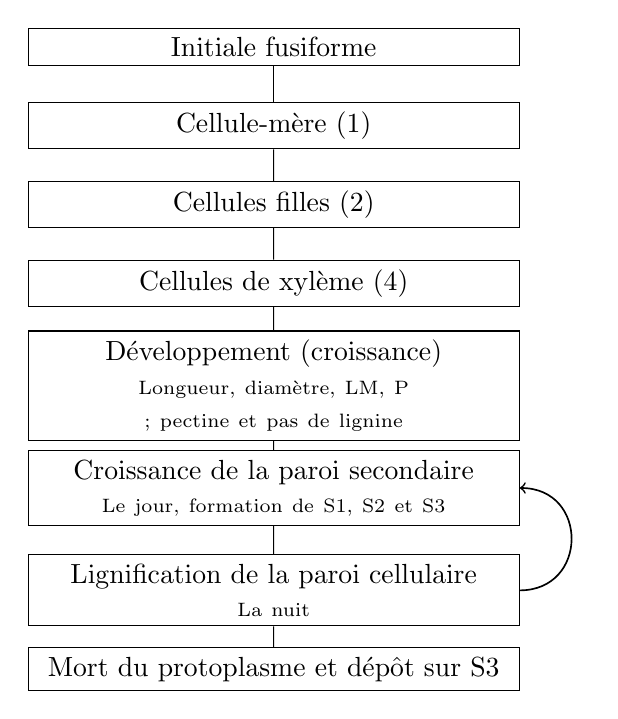
\begin{tikzpicture}[level distance=1cm, text width=6cm, align=center]
	\node[draw] {Initiale fusiforme}
	child {node[draw] {Cellule-mère (1)}
		child {node[draw] {Cellules filles (2)} 
			child {node[draw] {Cellules de xylème (4)} 
				child[level distance=1.3cm] {node[draw] {Développement (croissance) \\ {\scriptsize Longueur, diamètre, LM, P ; pectine et pas de lignine}} 
					child {node[draw](cr){Croissance de la paroi secondaire \\ {\scriptsize Le jour, formation de S\sub{1}, S\sub{2} et S\sub{3}}} 
						child {node[draw](li){Lignification de la paroi cellulaire \\ {\scriptsize La nuit}} 
							child[level distance=1cm] {node[draw] {Mort du protoplasme et dépôt sur S\sub{3}} } } } } } }
	};
	
	\draw[semithick,->] (li)..controls +(east:4) and +(east:4)..(cr);
	\end{tikzpicture}
	
	\caption{Mécanisme de croissance des cellules du bois à partir des divisons périclinales des initiales fusiformes du cambium.}
	\label{fig:mecacroissance}
\end{figure}

\subsection{Activité du cambium vasculaire selon la saison}

Le cambium est inactif en hiver. Au printemps, l'activité du cambium reprend si la température moyenne demeure supérieure à 5°C pour une semaine. La reprise de l'activité du cambium coïncide avec la production d'auxines par les méristèmes apicaux lors de l'ouverture des bourgeons. À l'automne, l'arrêt de l'activité du cambium est fonction de la photopériode.
%
%
%Références
%
%Benabdallah, B. 1996. Structure de la matière ligneuse.  Manuel de foresterie.  Ordre des ingénieurs forestiers du Québec et Presses de l'Université Laval. pp. 1276-1296. 
%Fahn, A. 1990.  Plant anatomy.  Fourth edition.  Pergamon Press, Oxford.  588 p.
%Jane, F.W. 1970. The structure of wood.  Second Edition.  Adam and Charles Black, London.  478 p.
%Panshin, A.J.; de Zeeuw, C. 1980.  Textbook of wood technology.  Fourth edition.  McGraw-Hill Book Co. New York.  722 p.

\chapter{La paroi cellulaire : composition chimique et structure}\label{paroi}

\begin{abstract}
Dans ce chapitre, nous présentons la structure hiérarchique du matériau bois, de l'échelle de la molécule à celle de la pièce de bois. Bien qu'il s'agisse d'un matériau complexe et variable, le bois n'est constitué en grande majorité que de trois types d'atomes, soit l'hydrogène, le carbone et l'oxygène. Ces atomes se groupent ensuite en trois grands types de molécules aux propriétés physico-mécaniques distinctes, soit la cellulose, les hémicelluloses et la lignine. Les chaînes de cellulose s'assemblent en cristallites, puis en microfibrilles qui, imprégnées dans une matrice de cellulose et d'hémicelluloses, forment ensuite la paroi cellulaire.
\end{abstract}

\minitoc

\section{Composantes chimiques de la paroi cellulaire}

Le bois est constitué de trois composantes principales :

\begin{description}
\item[La cellulose] qui donne au bois la majeure partie de sa résistance mécanique
\item[Les hémicelluloses] qui constituent la matrice dans laquelle on retrouve la cellulose
\item[La lignine] qui permet de \og coller \fg les cellules du bois entre-elles. 
\end{description} 

En plus de ces principaux constituants, on retrouve une quantité variable de composés organiques de faible poids moléculaire appelés \textbf{extractibles} pouvant se loger dans la paroi cellulaire et en réduire l'hygroscopicité et la perméabilité en plus d'affecter la couleur du bois et sa résistance aux champignons de dégradation. Des \textbf{constituants inorganiques} ou \textbf{cendres} sont également présents dans des proportions faibles variant de 0,1\% à 0,5\% de la masse anhydre. Le Tableau \ref{tab:composes} présente la composition chimique de la paroi cellulaire.\\

\begin{table}[!h]
\centering
	\begin{tabular}{l c c}
	\hline
	& \bf Résineux & \bf Feuillus \\
	\hline
	\hline
	Cellulose & 40 - 50 & 40 - 50 \\
	Hémicelluloses & 20 - 30 & 25 - 40 \\
	Lignine & 25 - 35 & 20 - 25 \\
	Extractibles &	0 - 25 & 0 -25 \\
	\hline
	\end{tabular}
\caption{Composition chimique de la paroi cellulaire du bois en proportion massique anhydre de la paroi cellulaire (\%) (adapté de \cite{choong1997wood})}
\label{tab:composes}
\end{table}

On qualifie souvent le bois de polymère car il est constitué de plusieurs composantes qui sont elles mêmes des polymères, c'est-à-dire des substances constituées par de grandes molécules formées par la répétition de plus petites unités structurales. Les polymères constituant la paroi cellulaire sont mélangés de façon ordonnée, cette organisation lui conférant ses propriétés mécaniques et par le fait même celles du bois.

\subsection{Cellulose}

La cellulose est la composante la plus importante du bois, autant en pourcentage de la masse anhydre que d'effet sur les propriétés mécaniques et l'hygroscopicité du bois. La cellulose est un polymère fibreux très stable chimiquement. Il est donc difficile de la modifier artificiellement pour en changer les propriétés. Il est aussi difficile d'isoler la cellulose pure car elle est étroitement liée avec d'autres polysaccharides, les hémicelluloses.\\

La cellulose (Figure \ref{fig:cellulose}) est un polymère contenant des molécules de longueurs différentes constituées d'une répétition de monomère appelés cellobiose. La cellobiose est l'unité de base de la cellulose et est constituée de deux cycles de glucose liés par des liaisons $\beta$-glycosidiques lui conférant ses propriétés structurales.\\


Chaque unité de cellobiose fait environ 1,03 nm de longueur et a des dimensions transversales de 0,84 x 0,79 nm dans les portions cristallines de la cellulose. Le degré de polymérisation de la cellulose, c'est-à-dire le nombre d'unités de glucose que l'on retrouve dans une molécule de cellulose, est d'environ \numprint{10000} dans la paroi secondaire des cellules du bois. Ceci correspond à une longueur moyenne de 5 \micro m pour la molécule de cellulose du bois.

\begin{figure}[h]
\centering
\includegraphics[scale=0.3]{img/cellulose}
\caption{La cellulose est un polymère monotone de cellobiose}
\label{fig:cellulose}
\end{figure}

La cellulose se présente sous forme cristalline dans les parois cellulaires, mais des zones amorphes sont aussi présentes. La cristallinité est une propiété d'un solide dont les constituants primaires sont disposés selon un motif régulier répété un grand nombre de fois. Les parties amorphes sont donc moins \og organisées \fg, ce qui leur confère de moins bonnes propriétés mécaniques et une plus grande hygroscopicité. 

Voici quelques faits saillant pour décrire la molécule de cellulose :

\begin{enumerate}
\item La molécule de cellulose a une forme rubanée,

\marginpar{L'amylase, le polymère de glucoses liés par des laisons $\alpha$ est une molécule de réserves énergétiques qui n'a pas de propriétés mécaniques}
\item les liaisons $\beta$-glycosidique donnent à la chaîne de cellulose une grande résistance mécanique. 

\item de nombreux groupements hydroxyles (--OH) sont disponibles le long de la chaîne de cellulose pour former des liaisons hydrogène latérales avec d'autres chaînes de cellulose tel qu'illustré à la Figure \ref{fig:cellulose_hydrogene}.\\
\end{enumerate}

Rappelons qu'une liaison hydrogène est de nature électrostatique. C'est une force intermoléculaire impliquant un atome d'hydrogène et un atome électronégatif comme l'oxygène. Ce sont également les groupements hydroxyles disponibles le long de la chaîne de cellulose qui en expliquent l'hygroscopicité.

% c'est faux
% et qu'elle consiste en la mise en commun d'un électron entre l'atome d'oxygène et l'atome d'hydrogène.
% Oui, t'as raison. Je le disais aux étudiant que c'était faux, mais je n'avais jamais pris le temps de le corriger. 

\begin{figure}[h]
\centering
\includegraphics[scale=0.8]{img/ch6_cellulose_hydrogene}
\caption{Liaisons hydrogène inter-moléculaires et intra-moléculaires entre deux molécules de cellulose}
\label{fig:cellulose_hydrogene}
\end{figure}

\subsection{Hémicelluloses}

% c'est faux
% Les hémicelluloses sont des polysaccharides  de composition semblable à la cellulose 
% AA: je pense qu'on devrait dires combien de C ont chacun des monomères décrits ici. 
Les hémicelluloses sont des polysaccharides de masse moléculaire beaucoup plus faible que la cellulose. Les monomères de l'hémicellulose peuvent être du xylose, du mannose, du galactose, du rhamnose ou de l'arabinose liée par des liaisons $\alpha$ ou $\beta$. Ils constituent de 20 à 35\% de la masse anhydre du bois et sont solubles dans les bases faibles et facilement hydrolysables dans les acides faibles pour former des sucres et des acides uroniques. Un groupe d'hémicelluloses appelés xylanes est dominant chez les feuillus et un autre groupe appelé glucomannanes est dominant chez les résineux.

\subsection{Lignine}

% Ce paragraphe est d'une complexité extraordinaire ! Tout tombe comme un cheveux sur la soupe. C'est quoi un procédé d'extraction ? C'est quoi la fraction remanente ? C'est quoi la lignine de Klason ? 
% AA; Ok, voilà qui est mieux je pense.
La lignine n'est formée que dans les parois cellulaires des plantes vivantes des spermatophytes, des ptéridophytes et des mousses. Le mot lignine vient du latin \textit{lignum} pour bois. On définit la lignine naturelle présente dans le bois comme un polymère tridimensionnel amorphe appelé protolignine produit dans la zone cambiale.\\

La lignine, quant à elle, réfère à la molécule que l'on peut extraire du bois à l'aide d'un procédé chimique (les plus connus sont les procédés Soda, sulfite et Kraft) ou thermique (pyrolyse). La distinction entre les termes lignine et protolignine vient du fait que les différent procédés d'extraction applicables altèrent la structure de la molécule. Il faut donc spécifier le procédé d'extraction utilisé lorsqu'on parle de lignine. Par exemple, suite à l'extraction à partir d'acides minéraux forts, on obtient la lignine dite \og de Klason \fg dont la structure générale est illustrée à la Figure~\ref{fig:lignine}. Elle consiste en un arrangement tridimensionnel complexe de noyaux phénoliques. Plusieurs groupements hydroxyles sont présents, ce qui résulte en une certaine hygroscopicité qui demeure tout de même bien inférieure à celle de la cellulose. On dit d'ailleurs que la lignine est \og partiellement hydrophobe \fg. La structure de la protolignine est légèrement différente de celle présentée à la Figure~\ref{fig:lignine} mais la structure générale est similaire. Il est aussi reconnu que la protolignine ne constitue pas un seul composé chimique mais un groupe de composés. La protolignine est différente entre les feuillus et les résineux et même entre les différentes espèces de feuillus et de résineux.\\

La protolignine est rigide mais remarquablement thermoplastique ou viscoélastique (Figure~\ref{fig:contrainte}), ce qui confère au bois la même propriété qui est exploitée dans le procédé de pressage à chaud des panneaux agglomérés à base de bois (180\textdegree C < T < 220\textdegree C) et lors du séchage à haute température (T > 100\textdegree C). Elle est produite dans la zone cambiale et est présente dans les cavités fines de la paroi cellulaire contribuant à en réduire l'hygroscopicité. La protolignine n'est pas distribuée uniformément dans la paroi cellulaire. On retrouve jusqu'à 70\% (base anhydre) de protolignine dans la lamelle moyenne composée entre les cellules. Cette proportion s'abaisse rapidement jusqu'à environ 10\% dans la paroi secondaire. Inversement, la teneur en cellulose est faible dans la lamelle moyenne composée et élevée dans la paroi secondaire.

\begin{figure}[h]
\centering
\includegraphics[scale=0.8]{img/ch6_lignine}
\caption{Description schématique de la structure de la lignine de Klason (d'après \cite{choong1997wood}).}
\label{fig:lignine}
\end{figure}

\begin{figure}[h]
\centering
\includegraphics[scale=0.5]{img/ch6_contrainte}
\caption{Viscoélasticité du bois due aux propriétés de la cellulose (composante élastique) et aux propriétés de la lignine (composante visqueuse).}
\label{fig:contrainte}
\end{figure}

\subsection{Substances extractibles}

Les substances extractibles peuvent être infiltrées dans les parois cellulaires ou déposées à la surface des lumens. Elles sont solubles dans l'eau chaude et/ou dans des solvants organiques (alcool, benzène). Les extractibles ne représentent généralement qu'une faible proportion de la masse anhydre du bois. Toutefois, ils peuvent représenter jusqu'à 35\% de la masse anhydre chez certains bois dont le quebracho \textit{(Schinopsis lorentzii Engl.}) très riche en tannin utilisé comme adhésif dans l'industrie des panneaux composites à base de bois dans quelques usines d'Amérique du Sud.\\

Les extractibles représentent une large gamme de composés organiques dont les polyphénols (ex. tannins) et les oléorésines (ex. térébenthine) sont les plus importants. On y retrouve aussi des gommes, graisses, acides gras, cires et hydrocarbures volatils. Ces produits sont responsables de plusieurs propriétés du bois dont l'odeur et la couleur du bois de duramen, la résistance aux champignons de pourriture et aux insectes, la perméabilité et la masse volumique. Comme les extractibles ne sont pas hygroscopiques, ils réduisent l'hygroscopicité du bois lorsqu'ils sont présents en forte proportion.

\subsection{Cendres}

Les cendres sont des composées inorganiques représentant environ 0,1 à 0,5\% de la masse anhydre du bois. On y retrouve principalement des composés à base de calcium, potassium, et magnésium. Le manganèse peut aussi être présent. Il est la cause des taches minérales chez les érables durs. La silice peut compter jusqu'à 2\% de la masse anhydre chez certaines espèces. Elle cause de graves problèmes d'usure prématurée des outils de coupe.

\section{Structure de la paroi cellulaire}

La paroi cellulaire est formée de structures rubanées appelées microfibrilles incrustées dans la lignine amorphe pour former une paroi cellulaire rigide. La structure des composantes de la paroi cellulaire sera décrite ci-dessous.

\begin{figure}[h]
\centering
\includegraphics[scale=0.55]{img/ch6_cellule}
\caption{Schéma bilan regroupant l'ensemble des éléments du chapitre}
\label{fig:grosschema}
\end{figure}

\subsection{Structure des microfibrilles}

Les microfibrilles sont des bandes ou rubans de polysaccharides visibles au microscope électronique. Elles sont souvent présentées comme les constituants de base de la paroi cellulaire, ce qui n'est pas tout à fait exact. En fait, on peut séparer les microfibrilles en unités appelées cristallites, qui font environ 60 nm de longueur et 3,5 $\times$ 10 nm en section transversale tel qu'illustré à la Figure \ref{fig:grosschema}. Chaque cristallite contient environ 50 chaînes de cellulose juxtaposées. Le terme cristallite réfère au fait qu'il s'agit d'une unité critalline de molécules de cellobiose agencées de manière régulière grâce aux liaisons hydrogène latérales entre les chaînes de cellulose.\\

On retrouve également des régions amorphes où les chaînes de cellulose ne sont pas liées par des liaisons hydrogène latérales. Ces régions amorphes sont donc les sites disponibles pour l\textbf{'eau liée} puisque des groupements hydroxyles libres sont présents. La sorption de l'eau liée dans les régions amorphes force les chaînes de cellulose à s'éloigner les unes des autres, ce qui résulte en un \textbf{gonflement de la paroi cellulaire}.


\subsection{Groupement des microfibrilles}

Les microfibrilles sont constituées de 3 à 25 cristallites formant une structure fibreuse. Les microfibrilles sont organisées entre elles en lamelles superposées dans une matrice de lignine et d'hémicellulose (Figure \ref{fig:grosschema}). Elles sont déposées à angle variable pour former la paroi cellulaire. Cette structure est analogue à celle du béton armé sauf qu'ici, la matrice est plastique. La grande élasticité de la cellulose pour des charges à court terme et la plasticité de la lignine pour des charges à long terme expliquent le comportement viscoélastique du bois.

\subsection{Porosité de la paroi cellulaire}

La paroi cellulaire est poreuse à cause du remplissage incomplet des espaces entre les microfibrilles par la lignine et les hémicelluloses. Cette porosité prend la forme de microcapillaires longs et étroits. Ces microcapillaires permettent à l'eau de pénétrer dans la paroi cellulaire. Ce réseau de capillaires occupe un volume maximal lorsque la paroi cellulaire est saturée d'eau. La masse volumique de la matière composant la paroi cellulaire varie de 1450 à 1500 kg/m\up{3}.

\subsection{Résumé de l'organisation des matériaux de base de la paroi cellulaire}
% Parler des crystallites de cellulose alors qu'on saute plein d'éléments contituants les parois ca me gène.
%AA: C'est mieux?

\begin{itemize}
\item La cellulose est un polymère dont l'unité de base est la cellobiose.
\item Les chaînes de cellulose contiennent des régions amorphes dans lesquels des groupements hydroxyles sont disponibles pour former des liaisons hydrogène avec des molécules d'eau. Elle contiennent également des zones critallines (les cristallites) au sein desquelles des liaisons hydrogène sont formées entre les chaînes, ce qui leur procure un arrangement parallèle.
\item Les cristallites sont organisés en longs “rubans” plus ou moins parallèles, groupés et imprégnés d'hémicelluloses partiellement liées à la cellulose. Le tout forme les microfibrilles.
\item La lignine et les extractibles sont ensuite déposés dans les microfibrilles de la paroi cellulaire.
\end{itemize}

\section{Les couches de la paroi cellulaire}

La paroi cellulaire est composée d'un ensemble de couches de structure différente. Une représentation schématique de la paroi cellulaire est présentée à la Figure \ref{fig:grosschema}. On y reconnaît la lamelle moyenne, la paroi primaire, les trois composantes de la paroi secondaire et la membrane verruqueuse. La Figure~\ref{fig:couches} vous procure une autre représentation de la même structure.

\begin{figure}[h]
	\centering
	\includegraphics[scale=0.7]{img/ch6_couches}
	\caption{Représentation schématique de la paroi cellulaire chez une trachéide de conifère. M: lamelle moyenne; P et P': paroi primaire; S\sub{1}: couche externe de la paroi secondaire; S\sub{2}: couche médiane de la paroi secondaire; S\sub{3}: couche interne de la paroi secondaire; W : membrane verruqueuse (d'après \cite{choong1997wood}).}
\label{fig:couches}
\end{figure}

\subsection{La lamelle moyenne}

La lamelle moyenne a pour fonction de cimenter les cellules adjacentes. Elle est isotrope et composée de substances amorphes telles que les pectines et la lignine. Les pectines, substances hautement polymérisées, sont sécrétées en quantité importante au cours du cloisonnement cellulaire. La teneur en lignine est faible chez les cellules proches du cambium et elle augmente pour devenir très importante à mesure qu'on s'en éloigne. La faible teneur en lignine de la lamelle moyenne près du cambium permet le développement des cellules du bois, la pectine étant relativement souple. L'épaisseur de la lamelle moyenne varie d'environ 0,2 à 2,0 \micro m.

\subsection{La paroi primaire}

La paroi primaire est la paroi de la cellule vivante en développement dès le méristème secondaire (cambium). La paroi primaire est fine et plastique chez la jeune cellule végétale, ce qui permet son développement à partir du cambium. La paroi primaire ne fait qu'environ 0,1 \micro m. Il est donc difficile, voir même impossible de la voir au microscope optique. On a donc défini la lamelle moyenne composée qui englobe la lamelle moyenne et les parois primaires de deux cellules adjacentes.

La paroi primaire est composée d'un peu de cellulose (9\%), d'hémicelluloses, de pectine, de lignine et d'eau (plus de 70\%), la lignine n'étant présente que chez les cellules matures. On retrouve donc peu de microfibrilles dans cette \og matrice \fg. En fait, elles n'occupent que 2,5 à 5,0\% du volume de la paroi primaire. L'orientation générale des microfibrilles de la paroi primaire est d'environ 85 par rapport à la direction axiale de la cellule.

\subsection{La paroi secondaire}

Une fois que la cellule a atteint sa taille maximale, la paroi \og grandit \fg vers l'intérieur en plusieurs couches: S\sub{1}, S\sub{2} et S\sub{3}. La matrice de lignine et d'hémicelluloses est beaucoup moins importante dans la paroi secondaire, la teneur en cellulose atteignant jusqu'à 94\% de la masse, ce qui confère au bois sa résistance mécanique. L'angle que font les microfibrilles avec la direction axiale des cellules varie pour les trois couches de la paroi secondaire. La croissance de la paroi secondaire serait cyclique, la cellulose étant produite le jour et la lignine la nuit.\\

Les ponctuations des trachéides, fibres et éléments de vaisseaux se mettent en place lors de la croissance de la paroi secondaire. Lorsque ces cellules ont terminé leur développement, le protoplasme (noyau + cytoplasme) meurt, ce qui n'est pas le cas pour les parenchymes qui demeurent en vie jusqu'à ce qu'il y ait duraminisation. Lorsque la paroi secondaire est mature, elle est dense et rigide. Il n'y a donc plus de croissance possible.

\subsection{Structure de la paroi secondaire}

\subsubsection{Couche externe de la paroi secondaire (S\sub{1})}

La couche externe de la paroi secondaire est une couche de transition entre la paroi primaire et la couche médiane de la paroi secondaire (S\sub{2}). Elle est mince (0,1 à 0,2 \micro m) et les microfibrilles y forment une spirale faisant un angle de 50 à 70\textdegree{} par rapport à la direction axiale de la cellule.

\subsubsection{Couche médiane de la paroi secondaire (S\sub{2})}

La couche médiane de la paroi secondaire est la plus importante autant en terme de volume qu'en terme d'impact sur les propriétés du bois. Son épaisseur varie de 1 à 5 \micro m et les microfibrilles y forment une spirale faisant un angle de 10 à 30\textdegree{} par rapport à la direction axiale de la cellule. À cause de cet angle faible des microfibrilles, la couche S\sub{2} change de dimension en épaisseur mais peu en longueur suite à la sorption de l'eau liée. L'angle des microfibrilles est beaucoup plus fort pour le bois juvénile et le bois de réaction que pour le bois adulte normal, ce qui explique la forte tendance au gauchissement de ce type de bois au séchage. L'épaisseur de la couche S\sub{2}  explique la variation de l'épaisseur de la paroi cellulaire entre le bois initial et le bois final.

\subsubsection{Couche interne de la paroi secondaire (S\sub{3})}\label{s3}

La couche interne de la paroi secondaire est mince (0,05 à 0,35 \micro m). Les microfibrilles y forment une spirale faisant un angle de 60 à 90\textdegree{} par rapport à la direction axiale de la cellule.

\subsubsection{Structure des parois cellulaires des parenchymes de xylème}

Il n'y a pas de paroi secondaire chez les parenchymes du xylème. On y retrouve plutôt des parois primaires \og épaissies \fg.\\

La proportion en volume des composantes de la paroi cellulaire est présentée au Tableau \ref{tab:proportionvolume}.

\begin{table}[ht]
\centering
	\begin{tabular}{c c}
	\hline
	\bf Composante & \bf Valeur \\
	\hline
	LMC & 2\% (constant) \\
	S\sub{1} & 10 à 20\% (variable) \\
	S\sub{2} & 68 à 78\% (variable) \\
	S\sub{3} &	8\% (constant) \\
	\hline
	\end{tabular}
\caption{Proportion en volume des composantes de la paroi cellulaire.}
\label{tab:proportionvolume}
\end{table}

\subsection{Distribution des constituants chimiques dans la paroi cellulaire}

La distribution des constituants chimiques dans la paroi cellulaire est présentée à la Figure~\ref{fig:prop}. On remarque que la teneur en lignine est maximale dans la lamelle moyenne composée et diminue vers l'intérieur de la cellule. Inversement, la teneur en cellulose est minimale dans la lamelle moyenne composée, maximale dans la couche S\sub{2} et diminue légèrement dans la couche S\sub{3}. La plus grande quantité de lignine se retrouve dans la couche S\sub{2} car elle est la plus épaisse bien que la teneur en lignine n'y soit pas très élevée.

\begin{figure}[h]
\centering
\includegraphics[scale=0.7]{img/ch6_prop}
\caption{Distribution des constituants chimiques de la paroi cellulaire (adapté de \cite{panshin1980textbook}).}
\label{fig:prop}
\end{figure}

\section{Notions complémentaires}

\subsection{Structure des ponctuations}

Les trois principaux types de ponctuations sont présentés à la Figure~\ref{fig:ponctuations2_rep}. On y reconnaît les ponctuations simples que l'on retrouve entre deux cellules de parenchyme, les ponctuations aréolées que l'on retrouve entre deux trachéides, deux éléments de vaisseaux ou deux fibres et les ponctuations semi-aréolées que l'on retrouve entre une cellule de parenchyme et une trachéide, un élément de vaisseau ou une fibre.
\\

Notons également les éléments suivants :

\begin{itemize}
\item le \og margo \fg d'une ponctuation aréolée chez les résineux est un réseau (filet) de paroi primaire flexible (pas de lamelle moyenne);
\item le \og torus \fg d'une ponctuation aréolée chez les résineux est un épaississement de la lamelle moyenne composée;
\item des incrustations se déposent sur le torus et la membrane de la ponctuation, surtout dans le bois de duramen, diminuant ainsi la perméabilité du bois.
\end{itemize}

\begin{figure}[!h]
	\centering
	\includegraphics[scale=0.7]{img/ch3_ponctuations2}
	\caption{Trois principaux types de ponctuations. a) ponctuation simple, b) ponctuation aréolée, c) ponctuation semi-aréolée.}
	\label{fig:ponctuations2_rep}
\end{figure}

\subsection{Impact des composantes chimiques sur les propriétés du bois et son utilisation}

\begin{multicols}{2}
\subsubsection{Cellulose}

\begin{itemize}
\item résistance à la traction longitudinale élevée
\item fabrication des pâtes et papiers
\item comportement élastique du bois
\end{itemize}			

\subsubsection{Lignine et hémicelluloses}
	
\begin{itemize}
\item cimentent les cellules et les microfibrilles entre elles
\item résistance mécanique générale du bois
\item comportement plastique du bois
\end{itemize}

\subsubsection{Hygroscopicité du bois}	

\begin{itemize}
\item cellulose (groupements --OH)
\item pectines et hémicelluloses sont hygroscopiques
\end{itemize}

\subsubsection{Gonflement et retrait}\label{gonflement}

\begin{itemize}
\item L < R < T
\item structure du bois
\item angle des microfibrilles dans la couche S\sub{2}
\end{itemize}

\todo{Référez-vous au schéma fait en classe pour expliquer l'effet de l'angle des microfibrilles sur l'ampleur des changements dimensionels dans chaque direction}

\subsubsection{Substances extractibles}
	
\begin{itemize}
\item stabilité dimensionnelle (peu hygroscopiques)
\item relations bois-eau
\item couleur, odeur
\item durabilité
\end{itemize}
\end{multicols}


%Références
%Fengel, D.; Wegener, G. 1989. Wood - chemistry, ultrastructure, reactions. Walter de Gruyter, Berlin. 613 p.
%Panshin, A.J.; de Zeeuw, C. 1980. Textbook of wood technology. Fourth edition. McGraw-Hill Book Co. New York. 722 p.
%Siau, J.F. 1995. Wood: Influence of moisture on physical properties. Department of Wood Science and Forest Products, Virginia Polythechnic Institute and State University. 227 p. 

\chapter{Variabilité du bois}\label{variabilite}

\begin{abstract}
Dans ce chapitre, nous décrivons la variabilité des propriétés du bois aux échelles suivantes: 1) dans un même cerne annuel, de la moëlle vers l'écorce et 3) selon la position au long de la tige. Nous nous attardons tant aux caractéristiques anatomiques (longueur et diamètre des cellules de bois) qu'à la composition chimique et aux propriétés physico-mécaniques. Un résumé de toutes le notions est inclus à la toute fin du chapitre.
\end{abstract}

\minitoc

\section{Introduction}

On fait souvent l'erreur de croire que le bois produit par des arbres de la même espèce est identique au niveau de sa structure et de ses caractéristiques physiques. En fait, le bois produit par des arbres de la même espèce et même le bois de deux pièces provenant du même arbre peut être très différent à plusieurs points de vue : masse volumique, accroissement annuel, dimension des cellules, épaisseur des parois cellulaires, constituants chimiques, angle des microfibrilles, nombre et taille des nœuds, rectitude du fil, résistance mécanique, perméabilité.\\

La \og qualité \fg du bois pour une utilisation donnée est déterminée par la variabilité d'une ou plusieurs de ces caractéristiques et de son impact sur cette utilisation. Les causes de ces variations peuvent se résumer comme suit :

\begin{enumerate}
\item Les changements du cambium vasculaire avec l'âge;
\item Le bagage génétique;
\item L'environnement.
\end{enumerate}

\section{Variabilité du bois à l'intérieur d'un arbre}

La variabilité du bois à l'intérieur des arbres et entre les arbres de la même espèce est encore peu connue pour les espèces commerciales résineuses et feuillues du Québec. Toutefois, des efforts de recherche sont présentement consentis dans ce domaine. La variabilité du bois dans un arbre dépend principalement de deux facteurs :

\begin{enumerate}
\item Le vieillissement du cambium;
\item Les variations de l'activité du cambium.
\end{enumerate}

\subsection{Variabilité des dimensions des cellules dans la section transversale des tiges}

Des variations importantes et claires sont observables chez les cellules où une élongation post-cambiale est présente, c'est-à-dire chez les trachéides, les fibres et les éléments de vaisseaux. Des variations moins accentuées sont observables dans la section des cellules, l'épaisseur des parois cellulaires et l'angle des microfibrilles dans les parois cellulaires.

\subsubsection{Longueur des trachéides des résineux et des fibres des feuillus dans le cerne annuel}

Les trachéides des résineux et les fibres des feuillus ont une longueur minimale dans le bois initial et maximale dans le bois final. La longueur est généralement en décroissance à la fin du cerne annuel (Figures ~\ref{fig:long_cerne} à \ref{fig:long_mfa_cerne}).

\begin{figure}[h]
	\centering
	\includegraphics[scale=0.8]{img/ch7_long_cerne}
	\caption{Variation de la longueur des cellules du bois initial au bois final à l'intérieur d'un cerne annuel. a) longueur des trachéides chez Pseudotsuga menziesii (résineux à transition abrupte), b) longueur des trachéides chez Pinus radiata (résineux à transition graduelle), c) longueur des fibres chez Catalpa bignonioides (feuillu à zone poreuse), d) longueur des fibres chez Populus tremuloides (feuillu à pores diffus) (adapté de \cite{panshin1980textbook})}
	\label{fig:long_cerne}
\end{figure}

\subsubsection{Longueur des éléments de vaisseaux dans le cerne annuel}

Chez les bois à zone poreuse, les éléments de vaisseaux sont courts dans le bois initial et longs dans le bois final (Figure~\ref{fig:long_fibres_cerne}). La longueur des éléments de vaisseaux est donc inversement proportionnelle au diamètre de ces derniers. Chez les bois à pores diffus, on observe une légère augmentation de la longueur des éléments de vaisseaux du bois initial au bois final (Figure~\ref{fig:long_diffus_cerne}).


\begin{figure}[h]
	\centering
	\includegraphics[scale=0.7]{img/ch7_long_fibres_cerne}
	\caption{Variation de la dimension des cellules à l'intérieur d'un cerne annuel de bois mature d'un bois feuillu à zone poreuse \textit{Fraxinus pennsylvanica} (adapté de \cite{panshin1980textbook})}
	\label{fig:long_fibres_cerne}
\end{figure}

\begin{figure}[h]
	\centering
	\includegraphics[scale=0.8]{img/ch7_long_diffus_cerne}
	\caption{Longueur des fibres et des éléments de vaisseaux à l'intérieur d’un cerne annuel de bois mature d'un bois feuillu à pores diffus, \textit{Fagus sylvatica} (adapté de \cite{panshin1980textbook})}
	\label{fig:long_diffus_cerne}
\end{figure}

\begin{figure}[h]
	\centering
	\includegraphics[scale=0.7]{img/ch7_long_mfa_cerne}
	\caption{Variation des dimensions des cellules et des angles des microfibrilles dans le cerne annuel d'un bois résineux à transition abrupte (adapté de \cite{panshin1980textbook})}
	\label{fig:long_mfa_cerne}
\end{figure} 


\subsubsection{Section des cellules dans le cerne annuel}

La section (surface) des cellules diminue du bois initial au bois final. Chez les résineux, en raison de l'alignement radial des trachéides, c'est la dimension des trachéides en direction radiale qui tend à varier (Figure~\ref{fig:resume_resineux}). Chez les feuillus à zone poreuse et semi-poreuse, on observe une diminution en diamètre des vaisseaux sans orientation particulière (Figure~\ref{fig:long_fibres_cerne}).

\subsubsection{Angle des microfibrilles des parois cellulaires dans le cerne annuel}

L'angle des microfibrilles des parois cellulaires est inversement proportionnel à la longueur des cellules. Il est donc maximal dans le bois initial et minimal dans le bois final (Figure~\ref{fig:long_mfa_cerne}).

\subsubsection{Variabilité de la structure du bois entre les cernes annuels}

On observe des variations nettes des caractéristiques du bois de la moelle vers l'écorce. Les causes de ces variations sont principalement :

\begin{enumerate}
\item Les changements des initiales du cambium avec le vieillissement de ce dernier;
\item le développement post-cambial des cellules.
\end{enumerate}

Cela engendre des variations dans :	

\begin{itemize}
\item dimensions des cellules;
\item structure de la paroi cellulaire incluant l'angle des microfibrilles;
\item proportion du volume occupé par différents types de cellules;
\item composition chimique des parois cellulaires.
\end{itemize}

Qui ont pour conséquences des changements dans les propriétés du bois :

\begin{itemize}
\item masse volumique;
\item résistance mécanique;
\item retrait et gonflement;
\item autres\ldots
\end{itemize}

Ces variations dans la section transversale en direction radiale et selon l'axe de la tige sont assez constantes d'une tige à l'autre, autant chez les résineux que chez les feuillus.

\subsubsection{Variation de la longueur des cellules dans le plan transversal des tiges}

On observe en général une élongation rapide des fibres et des trachéides dans les premières années de croissance (Figure~\ref{fig:long_moelle}). Il s'agit alors du bois juvénile. Suite à la période de production du bois juvénile, le cambium mature produit du bois selon les trois caractéristiques suivantes :

\begin{enumerate}
\item Stabilisation de la longueur des cellules;
\item Augmentation continue de la longueur des cellules;
\item Courbes paraboliques montrant une diminution de la longueur des cellules
\end{enumerate}

\begin{figure}[h]
	\centering
	\includegraphics[scale=0.7]{img/ch7_long_moelle}
	\caption{Courbes typiques illustrant la longueur des cellules de la moelle vers l'écorce (adapté de \cite{panshin1980textbook})}
	\label{fig:long_moelle}
\end{figure}


D'autre part, notons les points suivants :

\begin{itemize}
\item La période juvénile se termine habituellement après 10 à 20 ans dans le climat de l'Est du Canada. 
\item En général, la longueur des fibres et des trachéides diminue chez les arbres surannés. 
\item Les fibres et les trachéides sont toujours plus courtes dans le bois initial que dans le bois final.
\item La longueur des fibres et des trachéides varie en fonction de la hauteur dans l'arbre (Figure~\ref{fig:long_haut_resume}).
\item Les éléments de vaisseaux augmentent en longueur de la moelle vers l'écorce mais moins que les fibres puisque les éléments de vaisseaux croissent davantage en directions radiale et tangentielle dans la zone cambiale (Figure~\ref{fig:long_moelle_feuillus}).
\end{itemize}

La variation en longueur des éléments de vaisseaux, des fibres et des trachéides est due : 1) à la variation en longueur des initiales du cambium et 2) au développement post-cambial des cellules.

\begin{figure}[h]
	\centering
	\includegraphics[scale=0.7]{img/ch7_long_haut_resume}
	\caption{Variation de la longueur des trachéides selon la hauteur dans la tige pour le bois initial et le bois final dans une tige de pin rouge (\textit{Pinus resinosa}) de 35 ans. Les plus courtes trachéides se retrouvent au niveau du sol (S). La longueur des trachéides augmente rapidement jusqu'à une hauteur de 0,6 m. L'augmentation en longueur continue jusqu'à une longueur maximale sous la cime vivante (3,7 m) et décroît alors jusqu'au sommet de la cime vivante. Les courbes du bois initial montrent des trachéides plus courtes dans tous les cas (adapté de \cite{panshin1980textbook})}
	\label{fig:long_haut_resume}
\end{figure}

\begin{figure}[h]
	\centering
	\includegraphics[scale=0.7]{img/ch7_long_moelle_feuillus}
	\caption{Variation de la longueur des fibres et des éléments de vaisseaux de la moelle vers l'écorce (adapté de \cite{panshin1980textbook})}
	\label{fig:long_moelle_feuillus}
\end{figure}

\subsubsection{Variation du diamètre des cellules de la moelle vers l'écorce}

\begin{itemize}
	\item Chez les résineux, la section des trachéides augmente de la moelle vers l'écorce (Figure~\ref{fig:resume_resineux});
	\item Le volume des trachéides augmente de la moelle vers l'écorce puisque la section et la longueur augmentent;
	\item Chez les feuillus, les éléments de vaisseaux s'accroissent en diamètre de la moelle vers l'écorce, autant chez les bois à pores diffus qu'à zone poreuse; 
	\item Chez les feuillus, les fibres s'accroissent en diamètre modérément ou ce diamètre demeure constant de la moelle vers l'écorce, autant chez les bois à pores diffus qu'à zone poreuse.
\end{itemize}

\subsubsection{Variation de l'épaisseur des parois cellulaires de la moelle vers l'écorce}

Chez les résineux, l'épaisseur des parois du bois final augmente progressivement au moins jusqu'à 30 ans (environ 40\%), l'épaisseur des parois du bois initial augmente aussi mais de façon moins prononcée (environ 20\%) et on a une augmentation en épaisseur selon la direction radiale surtout.\\

Chez les feuillus on a une augmentation de l'épaisseur des parois de la moelle vers l'écorce.

\begin{figure}[h]
	\centering
	\includegraphics[scale=0.7]{img/ch7_resume_resineux}
	\caption{Variation des dimensions des trachéides de la moelle vers l'écorce chez de jeunes arbres de \textit{Pinus radiata} \cite{panshin1980textbook})}
	\label{fig:resume_resineux}
\end{figure}


\subsubsection{Variation de l'angle des microfibrilles de la moelle vers l'écorce}

L'angle des microfibrilles dans les parois cellulaires des trachéides et des fibres est inversement proportionnel à la longueur des cellules (Figure~\ref{fig:long_mfa_moelle}). Donc, l'angle des microfibrilles change de la moelle vers l'écorce avec les changements de longueur des trachéides ou des fibres.

\begin{figure}[h]
	\centering
	\includegraphics[scale=0.8]{img/ch7_long_mfa_moelle}
	\caption{Variation de la longueur des trachéides et de l'angle des microfibrilles de la moelle vers l'écorce dans les parois cellulaires de \textit{Cryptomeria japonica} (Cèdre du Japon ou Sugi) \cite{panshin1980textbook})}
	\label{fig:long_mfa_moelle}
\end{figure}

\subsection{Variabilité des dimensions des cellules selon la hauteur des tiges}

\subsubsection{Variation de la longueur des cellules selon la hauteur}

De façon générale, on peut dire que la longueur maximale des trachéides ou des fibres est localisée dans la partie extérieure du tronc, à environ 1/3 à 1/2 de la hauteur de l'arbre. Il y a des exceptions à cette règle. Par exemple, chez le sapin Douglas la longueur des trachéides augmente du bas vers le haut de l'arbre.

\subsubsection{Variation du diamètre des cellules}

En général, le diamètre des trachéides des résineux augmente de la souche jusqu'à environ le tiers à la demie de la hauteur de l'arbre et il diminue par la suite jusqu'au sommet de la cime vivante.\\

En général, le diamètre des fibres des feuillus diminue de la base jusqu'au sommet de la cime vivante.

\subsubsection{Variation de l'épaisseur des parois cellulaires}

L'épaisseur des parois cellulaires varie de la même façon que le diamètre des cellules, c'est-à-dire qu'en général, l'épaisseur des parois des trachéides des résineux augmente de la souche jusqu'à environ le tiers à la demie de la hauteur de l'arbre et elle diminue par la suite jusqu'au sommet de la cime vivante.\\

L'épaisseur des parois des fibres des feuillus diminue de la base jusqu'au sommet de la cime vivante.
%

%\begin{figure}[h]
%	\centering
	%	\includegraphics[scale=0.55]{img/ch6_cellule}
%	\caption{Variation de la longueur des fibres dans le plan longitudinal-radial d'une tige d'Eucalyptus regnans. Les deux côtés de la figure présentent les mêmes données de façon différente \cite{panshin1980textbook})}
%	%	\label{fig:grosschema}
%\end{figure}

\subsection{Dimensions des cellules dans les branches et les racines}

Les parties non commerciales des tiges (branches, racines, houppier) constituent environ 25\% de la masse anhydre des arbres. Il est donc pertinent de s'interroger sur les caractéristiques de ce bois.


\subsubsection{Variation des dimensions des cellules dans les branches}

Dans les résineux les trachéides sont significativement plus courtes dans les branches que dans la tige (50\% plus courtes) (Figure~\ref{fig:long_tige_branches}). Leur longueur atteint un maximum à environ un quart de la longueur de la branche et diminue par la suite.\\

Dans les feuillus la longueur des fibres des branches est d'environ 75\% de la longueur des fibres de la tige.

\subsubsection{Variations des dimensions des cellules dans les racines}

Dans les résineux, au collet, les trachéides sont courtes et il n'y a pas de variation radiale de longueur. La longueur des trachéides augmente du collet vers le bout des racines. Les trachéides des racines sont 50\% plus longues que celles de la tige en moyenne. Les trachéides des racines sont 30\% plus larges en direction tangentielle et les parois sont 15\% plus minces.

Dans les feuillus, les fibres des racines des feuillus sont environ 10\% plus courtes que celles des tiges.

\begin{figure}[h]
	\centering
	\includegraphics[scale=0.7]{img/ch7_long_tige_branches}
	\caption{Longueur des trachéides en fonction de l'âge cambial dans la tige et les branches de pin rouge (\textit{Pinus resinosa}) \cite{panshin1980textbook})}
	\label{fig:long_tige_branches}
\end{figure}

\section{Variation de la composition chimique des parois cellulaires}

\subsection{Polysaccharides}

\subsubsection{Teneur en cellulose}

Chez les résineux elle représente 40\% de la masse anhydre du bois initial et 50\% de la masse anhydre du bois final (Figure~\ref{fig:cellulose_cerne}). La cellulose du bois final possède un degré de polymérisation plus élevé et est plus cristalline que celle du bois initial. La teneur en cellulose des parois cellulaires augmente de la moelle vers l'écorce (45 à 65\% de la masse anhydre) (Figure~\ref{fig:cellulose_moelle}).

\subsubsection{Teneur en hémicelluloses}

Diminue de la moelle vers l'écorce (Figure~\ref{fig:cellulose_moelle}).

\subsection{Lignine}

Variations mineures en général. Elle varie de manière sinusoïdale dans le cerne annuel (Figure~\ref{fig:cellulose_cerne}) et tend à diminuer de la moelle vers l'écorce (Figure~\ref{fig:cellulose_moelle}).

\begin{figure}[h]
	\centering
	\includegraphics[scale=0.7]{img/ch7_cellulose_cerne}
	\caption{Variation de la teneur en cellulose et en lignine dans un cerne annuel de sapin Douglas (\textit{Pseudotsuga menziesii}) \cite{panshin1980textbook})}
	\label{fig:cellulose_cerne}
\end{figure}

\begin{figure}[h]
	\centering
	\includegraphics[scale=0.55]{img/ch7_cellulose_moelle}
	\caption{Distribution des composés chimiques de la paroi cellulaire de la moelle vers l'écorce chez les résineux \cite{panshin1980textbook})}
	\label{fig:cellulose_moelle}
\end{figure}


\section{Variation des propriétés physiques du bois}

\subsection{Variation de la masse volumique}

La masse volumique est définie comme la masse de matière par unité de volume. Elle est le plus important indicateur de qualité du bois et est principalement le résultat de variations de la structure cellulaire qui seront décrites ci-dessous.

\subsubsection{Variation de la masse volumique dans les cernes annuels}

Chez les résineux, la masse volumique est maximale dans le bois final et minimale dans le bois initial. La pente de la courbe $M_v$ en fonction de la position dans un cerne annuel dépend du type de transition bois initial / bois final. Le ratio $M_v$ bois final / $M_v$ bois initial = 2,5 à 5,0. Le bois initial est produit pendant la croissance des rameaux alors que la production d'auxines est maximale.  La transition bois initial / bois final correspond à l'arrêt de la croissance en longueur des rameaux.\\

L'augmentation de $M_v$ du bois final chez les résineux est principalement due à l'augmentation de l'épaisseur des parois cellulaires. Cette dernière résulte de la physiologie de l'arbre. Au début de la saison de croissance, les produits de la photosynthèse sont utilisés en priorité pour la croissance des rameaux et la production des aiguilles. Un minimum de substances nutritives est donc disponible au niveau du cambium.  En conséquence, les parois cellulaires demeurent minces jusqu'à ce que la croissance en longueur des rameaux cesse et que davantage de substances nutritives soient disponibles au niveau du cambium.

Chez les feuillus, la distribution des différents types de cellules (vaisseaux, fibres, parenchymes) détermine les variations de masse volumique dans le cerne annuel. De manière générale, la masse volumique est minimale dans le bois initial et maximale dans le bois final pour les feuillus à zone poreuse, à zone semi-poreuse et à pores diffus.
%
\subsubsection{Variation de la masse volumique de la moelle vers l'écorce}

Trois types :

\begin{description}
\item[Type I] Augmentation de $M_v$ de la moelle vers l'écorce;
\item[Type II] $M_v$ décroît à partir de la moelle mais s'accroît en s'approchant de l'écorce;
\item[Type III] $M_v$ décroît de la moelle vers l'écorce;
\end{description}


\subsubsection{Une espèce peut avoir différents types de comportement}

\textbf{Chez les résineux} les facteurs à considérer sont le diamètre des trachéides, l'épaisseur des parois et la proportion du cerne annuel occupée par le bois initial. Chez la plupart des espèces, la largeur de la bande de bois final varie moins que celle de bois initial (Figure~\ref{fig:larg_moelle}). On a donc des variations de $M_v$ (Figure~\ref{fig:densite_moelle}), car la proportion de bois final dans les cernes annuels change de la moelle vers l'écorce. L'épaisseur des parois augmente donc plus vite que le diamètre des trachéides.\\

\begin{figure}[h]
	\centering
	\includegraphics[scale=0.4]{img/ch7_larg_moelle}
	\caption{Largeur du bois initial et du bois final en fonction de la largeur totale du cerne chez l'épinette de Sitka \textit{Picea sitchensis} (\cite{moore2011wood})}
	\label{fig:larg_moelle}
\end{figure}

\begin{figure}[h]
	\centering
	\includegraphics[scale=0.5]{img/ch7_densite_moelle}
	\caption{Parton typique de variation de la masse volumique de la moelle vers l'écorce cerne chez l'épinette de Sitka \textit{Picea sitchensis}. Le gain de densité près ce l'écorce s'explique par une diminution de la largeur des cernes. Ce patron de variation correspond au Type II (graphique reproduit de \cite{moore2011wood})}
	\label{fig:densite_moelle}
\end{figure}

\textbf{Chez les feuillus à zone poreuse}, la proportion de bois final varie car la largeur du bois initial est plus ou moins constante d'un cerne à l'autre. Donc, si la largeur du cerne augmente, $M_v$ augmente et inversement (Figure~\ref{fig:densite_moelle_feuillus}).\\

\textbf{Chez les feuillus à pores diffus}, la proportion vaisseaux/fibres est le facteur déterminant (Figure~\ref{fig:densite_moelle_feuillus}). Le diamètre des vaisseaux augmente et le nombre de vaisseaux par unité de surface diminue de la moelle vers l'écorce. $M_v$ augmente si la proportion de fibres augmente. $M_v$ augmente si l'épaisseur des parois des fibres augmente. $M_v$ diminue si le diamètre des vaisseaux augmente avec une diminution de l'épaisseur des parois des fibres.

\begin{figure}[h]
	\centering
	\includegraphics[scale=0.55]{img/ch7_densite_moelle_feuillus}
	\caption{Variation de la moelle vers l'écorce à 1,5 m de hauteur de la masse volumique, de la proportion des cellules et de l'épaisseur des parois cellulaires pour un feuillu à zone poreuse (\textit{Celtis laevigata}) et un feuillu à pores diffus (\textit{Salix nigra}) \cite{panshin1980textbook})}
	\label{fig:densite_moelle_feuillus}
\end{figure}


\subsubsection{Variabilité de la masse volumique selon la hauteur dans les tiges}

Il s'agit de l'axe de variation le moins bien décrit. Chez les résineux, pour un même âge cambial, $M_v$ tend parfois à diminuer de la base de la tige vers le haut (Figure~\ref{fig:densite_haut_dave}). Chez les feuillus, il est difficile de décrire des tendances générales. Retenez que l'âge cambial \hyperref[croissance_cernes]{(qui varie en fonction de la hauteur dans l'arbre)}, est le facteur le plus important de variation des propriétés du bois en fonction de la hauteur dans la tige.\\

\begin{figure}[h]
	\centering
	\includegraphics[scale=0.5]{img/ch7_densite_haut_dave}
	\caption{Variation de la masse volumique des cernes de pin sylvestre (\textit{Pinus sylverstris}) en fonction de l'âge cambial et de la hauteur dans l'arbre \cite{auty2014models}). La ligne pleine représente la base de la tige (1.3 m) et les traits pointillés représentent des niveau qui s'élèvent successivement dans l'arbre.}
	\label{fig:densite_haut_dave}
\end{figure}


\section{Variabilité des propriétés physiques et mécaniques du bois}

Les principales propriétés physiques et mécaniques des principaux bois commerciaux du Québec sont présentées au Tableau~\ref{tab:grostab}. 

\subsection{Masse volumique basale}

Résineux : de 335 à 549 kg/m\up{3}, CV de l'ordre de 10\%

Feuillus : de 374 à 597 kg/m\up{3}, CV de l'ordre de 6\%

\subsection{Module d'élasticité en flexion}

Résineux : de 9650 à 14300 MPa, CV de l'ordre de 20\%

Feuillus : de 11200 à 14100 MPa, CV de l'ordre de 17\%

\subsection{Module d'élasticité en compression parallèle au fil}

Résineux : de 9720 à 12300 MPa, CV de l'ordre de 23\%

Feuillus : de 12700 à 15400 MPa, CV de l'ordre de 18\%

\begin{table}[ht]
\centering
	\begin{tabular}{l c c c c c c c}
	\hline
Espèce	&	Mv basale	&	$\beta$R	&	$\beta$T	&	$\beta$T/$\beta$R	&	MOE flex.//	&	MOE comp.//	&	Dureté\\
&	(kg/m\up{3})	&	(\%)	&	(\%)	&		&	(à 12 \% H)	&	(à 12\% H)	&	(à 12\% H)\\
&		&		&		&		&	(MPa)	&	(MPa)	&	(N)\\
\hline
\hline
Épinette blanche	&	354	&	3,2	&	6,9	&	2,2	&	9930	&	11400	&	1880\\
&	(10,2)	&		&		&		&	(18,6)	&	(23,7)	&	(16,5)\\
Épinette noire	&	406	&	3,8	&	7,5	&	2,0	&	10400	&	12300	&	2430\\
&	(9,4)	&		&		&		&	(22,3)	&	(23,0)	&	(16,4)\\
Pin gris	&	421	&	4,0	&	5,9	&	1,5	&	10200	&	10500	&	2560\\
&	(8,8)	&		&		&		&	(19,8)	&	(23,9)	&	(15,7)\\
Pin blanc	&	364	&	2,5	&	6,3	&	2,5	&	9380	&	9720	&	1650\\
&	(11,3)	&		&		&		&	(19,9)	&	(22,5)	&	(21,1)\\
Sapin baumier	&	335	&	2,7	&	7,5	&	2,8	&	9650	&	9720	&	1820\\
&	(8,0)	&		&		&		&	(14,3)	&	(19,8)	&	(16,6)\\
Mélèze laricin	&	549	&	2,8	&	6,2	&	2,2	&	14300	&	10500	&	4210\\
&	(11,9)	&		&		&		&	(14,1)	&	(27,6)	&	(21,3)\\
\hline
Érable à sucre	&	597	&	4,6	&	8,8	&	1,9	&	14100	&	15400	&	7290\\
&	(5,2)	&		&		&		&	(13,9)	&	(14,7)	&	(12,3)\\
Bouleau jaune	&	559	&	5,8	&	7,1	&	1,2	&	14100	&	15200	&	5930\\
&	(5,4)	&		&		&		&	(22,3)	&	(23,0)	&	(16,6)\\
Chêne rouge	&	581	&	3,6	&	6,7	&	1,9	&	11900	&	13700	&	6170\\
&	(5,1)	&		&		&		&	(14,0)	&	(14,3)	&	(13,2)\\
Frêne d’Amérique	&	570	&	4,2	&	7,0	&	1,7	&	12800	&	13500	&	7050\\
&	(8,4)	&		&		&		&	(19,9)	&	(21,8)	&	(21,5)\\
P. faux-tremble	&	374	&	3,6	&	6,6	&	1,8	&	11200	&	12700	&	2140\\
&	(6,4)	&		&		&		&	(17,1)	&	(17,8)	&	(14,2)\\
	\hline
	\end{tabular}
\caption{Propriétés physiques et mécaniques des principales espèces commerciales du Québec. Les nombres entre parenthèses désignent le coefficient de variation (\%) (Écart-type divisé par la moyenne $\times$ 100)}
\label{tab:grostab}
\end{table}

\subsection{Dureté}

Résineux : de 1650 à 4210 N, CV de l'ordre de 18\%

Feuillus : de 2140 à 7290 N, CV de l'ordre de 16\%

\subsection{Stabilité dimensionnelle}

La stabilité dimensionnelle d'un bois peut être estimée à partir du rapport $\beta_T$/$\beta_R$. Plus ce rapport se rapproche de l'unité, moins le bois a tendance à se déformer avec les changements de teneur en humidité. Donc, si on doit choisir un bois pour une application nécessitant une grande stabilité, on doit vérifier deux choses :

\begin{enumerate}
\item les coefficients de retrait radial et tangentiel doivent être minimum.
\item le rapport $\beta_T$/$\beta_R$ doit aussi être minimum.
\end{enumerate}

$\beta_T$ est environ égal à $2\beta_R$. Il y a au moins deux théories pour expliquer cet état de chose. (1) L'effet des parois cellulaires du bois final : il y a plus de matière en direction tangentielle dans le bois final donc il y a plus de retrait en direction tangentielle. (2) Effet des rayons : les rayons constituent des structures ayant pour effet de limiter le retrait radial.

% ATTENTION : BIEN RELIRE CA parce que plein de symboles ont disparus
% Ok, c'est bon je crois

\section{Bilan}

Le tableau \ref{tab:bilan} résume l'ensemble des élément vus dans ce chapitre.

\begin{table}[p]

	\scriptsize
	
	\begin{tabular}{|b{0.4cm}|b{0.4cm}| m{4cm} m{4cm} m{4cm}|}
	
	\hline  &  & \bf Variation à l’intérieur des cernes annuels & \bf Variation entre les cernes annuels (section transversale) &  \bf Variation selon la hauteur \\ 
	\hline  \flip{\hspace{-0.7cm} \large Résineux} & \flip{\hspace{-0.65cm}\normalsize Trachéides} & 
	
	\begin{description}[leftmargin=0.2cm]
	\item[longueur] min. b.i.;  max. b.f.; 15\%
	\item[diamètre radial]  max. b.i.; min. b.f. 
	\item[angle microfibrilles] max. b.i.;  min. b.f.
	\item[teneur en cellulose]  min. b.i.;  max. b.f.
	\item[teneur en lignine] varie très peu
	\item[teneur en extractibles] diminue radialement
	\item[épaisseur des parois] min. b.i.;  max. b.f.
	\end{description}
	
	& 
	
	\begin{description}[leftmargin=0.2cm]
	\item[longueur] augmente dans les premières années de croissance; toujours plus court dans le b.i. que dans le b.f.
	\item[diamètre radial] augmente de la moelle vers l'écorce
	\item[diamètre tangentiel] augmente de la moelle vers l'écorce
	\item[épaisseur des parois] b.i.: augmente de la moelle vers l'écorce (20\%); b.f.: augmente de la moelle vers l'écorce ($\Delta$e  40\%).
	\item[angle microfibrilles] diminue de la moelle vers l'écorce
	\item[teneur en cellulose] augmente de la moelle vers l'écorce d'environ 45 à 65\% de $M_0$.
	\item[teneur en lignine] varie très peu
	\item[teneur en hémicelluloses] diminue de la moelle vers l'écorce
	\item[teneur en extractibles] diminue de la moelle vers l'écorce
	\end{description} 
	
	& 
	
	\begin{description}[leftmargin=0.2cm]
	\item[longueur] augmente de la souche vers la base de la cime et diminue par la suite jusqu'au sommet de l'arbre.
	\item[diamètre] augmente de la souche vers la base de la cime et diminue par la suite jusqu'au sommet de l'arbre.
	\item[épaisseur des parois] augmente de la souche vers la base de la cime et diminue par la suite jusqu'au sommet de l'arbre.
	\end{description} \\ 
	
	\hline \multirow{2}*{\flip{\large Feuillus \qquad}}  & \flip{\hspace{-0.7cm} \normalsize Vaisseaux} & 
	
	\begin{description}[leftmargin=0.2cm]
	\item[longueur] min. b.i.; max. b.f.;  l  10\% ou moins
	\item[diamètre] max. b.i.; min. b.f. chez les bois à zone poreuse et à pores semi-diffus
	\end{description}
	
	& 
	
	\begin{description}[leftmargin=0.2cm]
	\item[longueur] augmente de la moelle vers l'écorce
	\item[diamètre] augmente de la moelle vers l'écorce
	\item[angle microfibrilles] diminue de la moelle vers l'écorce
	\end{description}
	
	&  \\ 

	
	\cline{2-5} & \flip{\hspace{-0.5cm}  \normalsize Fibres} & 
	
	\begin{description}[leftmargin=0.2cm]
	\item[longueur] min. b.i.;  max. b.f.; l  30 à 100\%
	\item[angle microfibrilles] max. b.i.; min. b.f.
	\end{description} 
	
	& 
	
	\begin{description}[leftmargin=0.2cm]
	\item[longueur] augmente radialement
	\item[épaisseur des parois] augmente de la moelle vers l'écorce
	\item[angle microfibrilles] diminue de la moelle vers l'écorce
	\end{description}
	
	&  
	
	\begin{description}[leftmargin=0.2cm]
	\item[longueur] augmente de la souche vers la base de la cime et diminue par la suite jusqu'au sommet de l'arbre.
	\item[diamètre] diminue de la souche jusqu'au sommet de l'arbre
	\item[épaisseur des parois] diminue de la souche jusqu'au sommet de l'arbre
	\end{description}\\ 
	\hline 
	\end{tabular} 
	
	\caption{Tableau résumé de notions vues dans ce chapitre}
	\label{tab:bilan}
\end{table}


%Références
%
%
%
%Panshin, A.J.; de Zeeuw, C. 1980. Textbook of wood technology. Fourth edition. McGraw-Hill Book Co. New York. 722 p. 
%
%
%
%Jessome, A.P. 1977. Strength and related properties of woods grown in Canada. Forintek Canada Corp. 37 p.

\chapter{Sylviculture et qualité du bois}

\begin{abstract}
	Dans ce chapitre nous définissons d'abord le concept de qualité du bois. Nous faisons ensuite un bref survol des différents travaux sylvicoles à la disposition des forestier pour cultiver et régénérer la forêt. Finalement, les bases permettant d'estimer les effets des traitements sylvicoles sur la qualité du bois sont présentées.
\end{abstract}

\minitoc

\section{Le concept de qualité du bois}

On peut définir la qualité du bois comme une série d’attributs qui rendent le bois approprié pour des usages donnés. \textbf{Le concept de \og qualité \fg du bois n'est pas absolu, mais relatif à un produit donné}.

Quelques caractéristiques du bois sont désirables pour certains usages mais indésirables pour d’autres. Par exemple, pour le bois de charpente, on recherche du bois rigide, présentant une bonne résistance mécanique associée à des nœuds de petite taille et à un fil droit (\textit{Pseudotsuga menziesii; Picea spp.}). Pour la sculpture, on recherche des bois stables, tendres et de masse volumique homogène (\textit{Chamaecyparis nootkatensis; Tilia americana}). Pour le revêtement des planchers et le meubles, on recherche des bois de dureté élevée et de couleur appréciée des consommateurs (\textit{Acer spp., Quercus spp., Betula alleghaniensis, Fraxinus americana}…). Pour la fabrication du papier on recherche du bois possédant des fibres longues à parois cellulaires minces, l’affaissement des parois cellulaires donnant un papier moins poreux mais plus résistant mécaniquement.

\section{Les bases de la sylviculture}
\subsection{Définition de la sylviculture}
On peut définir la sylviculture comme la science qui vise à cultiver la forêt pour en retirer le maximum de biens et de services pour la collectivité. Elle consiste en un ensemble de techniques visant à modeler les caractéristiques des peuplements forestiers de manière à ce qu'ils répondent mieux aux objectifs d'aménagement qu'on leur a fixés. Pour ce faire, elle utilise divers moyens, dont la récolte, la régénération et les différents soin d'éducation. 

\subsection{Procédés de régénération de la forêt}
Les \og précédés de régénération \fg font référence à la coupe forestière qui, d'un point de vue sylvicole, servent à régénérer la forêt. Évidemment, dans le contexte plus large de l'aménagement forestier, on les pratique dans le but d'approvisionner une ou des usines de transformation.

\subsubsection{La coupe totale}\label{cprs}

Dans la méthode par coupe totale, la régénération du peuplement est prévue à la toute fin de la révolution, après l'abattage en coupe unique de tous les arbres contenus dans la superficie à régénérer (Figure \ref{fig:CPRS}). L'expression \og coupe avec protection de la régénération (CPRS) a été popularisée au Québec pour désigner une approche qui consiste à protéger la régénération préexistante lors des opérations de récolte. L'approche consiste à utiliser un système de sentiers dans lesquels la machinerie circule. Ainsi, seule une partie de la régénération préétablie (et du sol) est perturbée par les opérations.\\

\begin{figure}[!h]
\centering
\includegraphics[width=0.7\linewidth]{./img/ch8_CPRS}
\caption{Procédé de régénération par coupe totale. Le système de sentiers de récolte permet de protéger la régénération. CPRS = coupe avec protection de la régénération et des sols}
\label{fig:CPRS}
\end{figure}

Évidemment, dans le cas de la coupe totale, l'ensemble des tiges de diamètre marchand sont envoyées à l'usine de transformation en une seule étape. La qualité des approvisionnements dépend donc des caractéristiques du peuplement au moment de la coupe.

\subsubsection{L'établissement de la régénération par coupe progressive}\label{cprog}

La caractéristique la plus fondamentale de la régénération par coupes progressives réside dans le fait que l'établissement du nouveau peuplement débute \textbf{avant la fin de la révolution du peuplement en place}. Ainsi, les semis installés profitent de la protection d'un couvert forestier pendant quelques années. Ce procédé conduit à la récolte complète du peuplement à travers une série de coupes partielles qui surviennent en fin de révolution (Figure \ref{fig:cprog}). Le principe du procédé veut que le peuplement soit ouvert de façon progressive pour favoriser l'établissement et le développement des jeunes semis, tout en donnant à ceux-ci une protection suffisante en présence de conditions adverses. Dans ce procédé, on considère deux types de coupes: la coupe d'ensemencement et la coupe finale.

\begin{description}
\item[La coupe d'ensemencement] La coupe d'ensemencement, tout en favorisant aussi une bonne production de graines, vise principalement à obtenir un éclairement au sol propice à la germination et à l'installation des espèces désirables. On favorise le plus possible la rétention des arbres des essences recherchées (qui servent d'apport de semences) aux dépens des autres.\\ 

Ainsi, le choix des arbres lors de cette coupe dite \og partielle \fg aura une influence sur la qualité des approvisionnements. Ceux-ci seront possiblement constitués d'une proportion plus élevée d'essences peu désirées par rapport à la coupe finale. Comme il y a un délai de quelques années entre les deux coupes, la taille moyenne des arbres sera aussi plus faible que lors de la coupe finale. 

\item[La coupe finale] : C'est la dernière coupe qui élimine tous les grands arbres encore en place. Elle vise à donner la pleine lumière au nouveau peuplement. Il s'agit en fait d'une \hyperref[cprs]{CPRS}.
\end{description}

\begin{figure}[!h]
\centering
\includegraphics[width=1\linewidth]{./img/ch8_CPI}
\caption{ Procédé de régénération par coupe progressive}
\label{fig:cprog}
\end{figure}


\subsubsection{La coupe de jardinage}

Certains peuplement forestiers contiennent des arbres de tous les âges, et donc de toutes les tailles. C'est couvent le cas dans nos forêts feuillues tempérées. Dans ce contexte, la coupe de jardinage permet d'assurer la régénération, la récolte et l'éducation du peuplement dans une seule intervention. Elle vise à établir ou maintenir une structure dite \og inéquienne \fg dans le peuplement.\\

En principe, les arbres sont récoltés à mesure qu'ils arrivent à maturité, ce qui crée une trouée dans le couvert. Ils seront remplacés par des semis déjà à leur place au moment de la coupe ou par une nouvelle cohorte de semis qui s'établissent et se développent en profitant de nouvelles conditions plus favorables (nouvel apport de lumière au sol).\\

Une partie seulement du peuplement est enlevée, de sorte qu'on peut le perpétuer indéfiniment et, s'il est appliqué selon les règles de l'art, extraire périodiquement des tiges de haute qualité et de dimension désirées. Les règles de l'art dictent que ce sont les arbres de faible vigueur qui devraient être récoltés en priorité, puisque ceux-ci sont susceptibles d'être morts lors de la prochaine intervention. En procédant à l'inverse, c'est-à-dire en choisissant les tiges de meilleure qualité, souvent vigoureuses, on procède à un écrémage progressif de la forêt. La ligne est donc mince entre la nécessité d'approvisionner une usine en bois de qualité dans l'immédiat et de maintenir le capital forestier nécessaire à la production de tiges de qualité dans l'avenir.\\
	
Dans une \textbf{coupe de jardinage} théoriquement, chaque groupe de structure équienne composant le peuplement de structure inéquienne occupe la place d'un arbre enlevé à maturité (Figure \ref{fig:jardinage_pied}). Immédiatement après la coupe, quelques milliers de semis sont installés dans la trouée laissée par un seul arbre récolté. Au stade du gaulis, quelques centaines d'individus demeurent et leur nombre diminuera jusqu'à quelques dizaines de perches par la suite. Lors de l'intervention, la récolte devrait théoriquement s'effectuer dans chacun des \hyperref[developpement]{stades de développement} du peuplement (Figure~\ref{fig:jardinage}).
	
	\begin{figure}[!h]
		\centering
		\includegraphics[width=0.6\linewidth]{./img/ch8_jardinage_pied}
		\caption{Théoriquement, dans le jardinage par pied d'arbre, chaque groupe de structure équienne composant le peuplement de structure inéquienne occupe la place d'un arbre enlevé à maturité}
		\label{fig:jardinage_pied}
	\end{figure}
	
	\begin{figure}[!h]
		\centering
		\includegraphics[width=1\linewidth]{./img/ch8_jardinage}
		\caption{Procédé de régénération par coupe de jardinage par pied d'arbre}
		\label{fig:jardinage}
	\end{figure}	


Au Québec, on peut dire que le potentiel de ce procédé de régénération a été démontré à une échelle expérimentale, mais que la possibilité de l'appliquer avec succès à l'échelle industrielle reste à démontrer. C'est face à ce constat que la méthode MSCR qui guide l'évaluation de la vigueur des arbres a été développée.\\

Le guide contient une grille d'évolution des défauts des arbres permettant d'évaluer la priorité de récolte. Celle-ci est basée sur plusieurs éléments qui doivent être vérifiés par le marteleur. L'identification de l'essence, du défaut externe le plus important, de l'endroit où siège ce défaut ainsi que l'origine de celui-ci constitue la première étape à franchir pour identifier la classe de vigueur actuelle de l'arbre. Cette information permet alors d'identifier la priorité de récolte des tiges.\\

Il existe 4 niveaux de vigueur qui se définissent ainsi \citep{boulet2007defauts} :

\begin{itemize}
	\item Priorité 1 - \textbf{M, mourir} : Tige très défectueuse, qui risque de se renverser, de se rompre ou de mourir sur pied avant la prochaine rotation. Arbre moribond ou en perdition.
	\item Priorité 2 - \textbf{S, survie} : Tige défectueuse en perdition dont le volume de bois risque de diminuer en raison de la carie, mais dont la survie n'est pas compromise avant la prochaine rotation. Arbre en décroissance.
	\item Priorité 3 - \textbf{C, conservé} : Tige peu défectueuse à conserver, dont le volume de bois marchand ne risque pas de se dégrader avant la prochaine rotation. Arbre en croissance.
	\item Priorité 4 – \textbf{R, réserve }: Tige saine en réserve idéalement dégagée pour croître librement, qui constitue le capital forestier de premier choix. Arbre d'avenir en réserve.	
\end{itemize}

Notez que cette classification ne tient pas directement compte de la qualité du bois. Elle cherche seulement à évaluer la probabilité qu'une tige soit vivante lors du prochain passage dans le peuplement (la prochaine coupe prévue dans 20 ou 25 ans dans le cas du jardinage). Une fois cette probabilité établie, on doit récolter les tiges les plus susceptibles de mourir rapidement. Afin d'assurer la rentabilité du traitement sylvicole, il importe de récolter en priorité les arbres non vigoureux ayant conservé une qualité suffisante pour le sciage.\\

\subsubsection{Classes de qualité (A-B-C-D)}
Au Québec, la détermination de classes de qualité sur les arbres debout s'applique surtout au feuillus puisque la \og qualité \fg des tiges pour le sciage et le déroulage (qui mènent à des produits à haute valeur ajoutée) diffère grandement entre les individus, contrairement aux résineux. La classification est inspirée des normes de classification des billes (bois abattus). Ces dernières servent au calcul des droits de coupe que doivent verser les compagnies œuvrant sur terres publiques \citep{MRNF2009taux}. Chez les résineux du groupe SEPM (sapin, épinettes, pin gris, mélèze), il n'existait jusqu'à tout récemment qu'une seule classe de qualité. Le bois de ces essences provenant des terres publiques est donc vendu sans égard direct à sa qualité.\\ 

Pour plusieurs autres essences, dont en particulier les bois feuillus, les normes de mesurage sont beaucoup plus complexes. Dans ce cas, la qualité du bois influence le prix auquel le bois provenant des forêts publiques est vendu aux industries forestières. Les détails de ces normes de mesurage vont bien au-delà des objectifs visés par ce cours. Notons tout de même que les droits de coupe peuvent s'élever à plus de 70\$/m$^3$ pour du bois de déroulage feuillu alors qu'ils peuvent être seulement de 0,40\$/m$^3$ pour le bois à pâte. Afin d'obtenir une idée préalable de la qualité du capital forestier sur pied, le gouvernement du Québec s'est doté d'un système de classification de la qualité des tiges d'essences feuillues.\\

Le document du MRNQ sur la Classification des tiges d'essences feuillues, normes techniques (SIF, document FQ91-3008) définit des critères pour le classement de la qualité des tiges en fonction de leurs utilisations potentielles (Figure~\ref{fig:Monger}). L'évaluation de la qualité s'effectue seulement sur les arbres vivants debout, d'essences feuillues commerciales et ayant un diamètre à hauteur de poitrine (dhp) supérieur à 23 cm. Le principe général consiste à:

\begin{enumerate}
	\item à trouver le meilleur 3,7 m à l'intérieur des premiers 5 m à la base de la tige;
	\item à séparer la bille en quartiers égaux (face de l'arbre sur ¼ de la circonférence);
	\item à identifier la 3e face en qualité (2e pire!);
	\item à estimer les débits clairs sur cette face;
	\item à calculer des réductions attribuables à certains défauts ou à la courbure de la tige.
\end{enumerate}	

\begin{figure}[ht]
	\centering
	\includegraphics[width=0.5\linewidth]{img/ch8_Monger}
	\caption{Illustration du principe utilisé par le système de classification de la qualité des tiges d'essences feuillues. Le système est en vigueur au Québec depuis plusieurs décennies. Il permet d'estimer la valeur des bois sur pied, comme nous l'avons fait dans \cite{hassegawa2015large} \url{http://bit.ly/1gf2UNf}.}
	\label{fig:Monger}
\end{figure}

\subsection{La phase d'établissement du peuplement}

Lorsqu'on vise la régénération d'un peuplement forestier, on fait le choix entre la régénération naturelle ou le reboisement (plantation). Ces choix peuvent évidemment affecter la composition forestière (mélange d'espèces), ce qui aura éventuellement un impact sur les approvisionnements forestiers. Les choix qui sont effectués lors de cette phase n'auront toutefois qu'un impact à long terme sur les approvisionnements aux usines.

\subsubsection{La régénération naturelle}

La régénération naturelle est la méthode de régénération la plus opportuniste puisqu'on profite des éléments déjà en place. Ainsi, il est possible d'assurer la régénération du peuplement de façon économique. De plus, en utilisant l'ancien peuplement, on a plus de chances de régénérer des essences et des arbres mieux adaptés aux conditions de la station. Par contre, lorsque le capital sur pied est peu intéressant, il est possible que la régénération naturelle ne soit pas souhaitable. Au Québec, sur terres publiques, on a choisi de miser en priorité sur l'établissement d'une régénération naturelle.\\

\subsubsection{La régénération artificielle}

La régénération artificielle permet de remettre en production les superficies peu ou mal régénérées naturellement, soit 15 à 18\% des superficies exploitées au Québec \citep{thiffault2003sylviculture}. Grâce à l'utilisation d'espèces à croissance rapide ou de semences améliorées génétiquement, les plantations permettent d'augmenter le rendement des forêts. Ce rendement accru peut, en contrepartie, causer un déclin des propriétés du bois telles que la masse volumique chez les résineux, par exemple. Toutefois, les programmes de sélection génétique ont contribué à produire des plants à la fois hautement productifs et aux propriétés du bois désirables.\\

Après avoir choisi les plants à utiliser, le forestier doit déterminer la densité de reboisement. Les facteurs à prendre en compte sont alors la forme de la tige, la mortalité et la grosseur des branches, la qualité du bois, la production à l'hectare ainsi que par arbre, la survie, la stabilité de la plantation, la rentabilité des éclaircies et les aspects économiques. Cependant, presque toutes les études économiques ont convergé vers de très faibles valeurs de densité optimale \citep{thiffault2003sylviculture}. Au Québec, la densité préconisée (en forêt résineuse) est de 2000 tiges ha\up{-1}.\\

\subsection{Les travaux d'éducation des semis}

Le but premier du sylviculteur qui établit un nouveau peuplement forestier est d'assurer l'établissement d'un régénération libre de croître et occupant l'ensemble du site. Différents travaux peuvent être appliqués lorsque ces conditions ne sont pas réunies (Figure~\ref{fig:debrous}).\\

Pour combler les espaces inoccupés, deux actions sont possibles: le regarni et l'enrichissement. Le premier s'adresse aux peuplements reboisés ou ensemencés pour "garnir à nouveau". L'enrichissement permet d'introduire de nouvelles essences plus résistantes, plus performantes ou plus rentables. À titre d'exemple, c'est le cas lorsqu'on introduit de l'épinette blanche dans la régénération de sapin baumier ou encore du chêne rouge ou du pin blanc dans la régénération d'érable à sucre et de hêtre. Le dépressage est la simple action de réduire la densité. Cette opération est souvent faite systématiquement à ce stade. 


\begin{figure}[!h]
	\centering
	\includegraphics[width=1\linewidth]{./img/ch8_debrous}
	\caption{Différents travaux d'éducation au stade semis}
	\label{fig:debrous}
\end{figure}



\subsection{Les travaux précommerciaux}

Le nettoiement, le dépressage et le dégagement  au stade gaulis constituent trois types d'interventions que l'on regroupe au Québec dans la catégorie des « éclaircies précommerciales » (Figure \ref{fig:precom}). Elles sont très régulièrement appliquées au Québec. Elles ont deux impacts principaux sur la qualité future est approvisionnements: 1) elles permettent de contrôler la composition en espèces; 2) elles donnent plus de lumière aux arbres résiduels, ce qui leur permet de développer une cime plus vigoureuse.\\

\begin{figure}[!h]
	\centering
	\includegraphics[width=1\linewidth]{./img/ch8_precom}
	\caption{Différents types d'éclaircies précommerciales au stade gaulis}
	\label{fig:precom}
\end{figure}

\subsection{Les travaux d'éclaircie commerciale}\label{ecomm}

L'éclaircie est dite « commerciale » lorsque les tiges coupées sont d'assez bonnes dimensions pour être transformées. Retenons deux systèmes d'éclaircies généralement reconnus dans la littérature : l'éclaircie par le bas et l'éclaircie par le haut.\\

\subsubsection{Éclaircie par le bas}

L'éclaircie par le bas consiste à retirer les tiges des classes intermédiaires et opprimées (voir figure \ref{fig:bas}). Elle permet de récupérer la mortalité imminente des tiges. Ainsi, l'approvisionnement associé à ce traitement sera surtout constitué de petites tiges peu vigoureuses et possiblement mal formées. Il s'agit d'un sacrifice à faire dans l'immédiat pour l'amélioration de la qualité et de la taille des tiges du peuplement lors de la coupe finale.\\ 

\begin{figure}[!h]
	\centering
	\includegraphics[width=1\linewidth]{./img/ch8_bas}
	\caption{Éclaircie par le bas}
	\label{fig:bas}
\end{figure}

\subsubsection{Éclaircie par le haut}

L'éclaircie par le haut consiste à éliminer un nombre déterminé de tiges des étages supérieurs afin de diminuer la densité du peuplement et de favoriser le développement des tiges d'avenir. Cette technique d'éclaircie est particulièrement utile pour stimuler le plus possible la croissance des tiges d'avenir \citep{smith1997practice} (voir Figure \ref{fig:haut}).\\

L'éclaircie par le haut diffère de l'éclaircie par le bas de deux façons : 1) elle s'applique à l'étage supérieur et 2) les tiges opprimées et intermédiaires qui ne gênent pas les tiges d'avenir demeurent en tout temps conservées dans le peuplement. Le fait de conserver l'étage inférieur possède plusieurs avantages dont celui d'éduquer les tiges d'avenir. La présence de voisins limite le développement de grosses branches (qui formeront de gros nœuds) dans les étages inférieurs.

\begin{figure}[!h]
	\centering
	\includegraphics[width=1\linewidth]{./img/ch8_haut}
	\caption{Éclaircie par le haut}
	\label{fig:haut}
\end{figure}


\subsection{Choix du moment d'éclaircie}

Plusieurs moyens, à la fois qualitatifs ou quantitatifs, peuvent être utilisés pour déterminer le moment d'éclaircir. Le pourcentage de cime vivante est souvent utilisé comme indice. Si le pourcentage de cime vivante se situe entre la demie et le cinquième de la longueur des arbres, il est temps d'effectuer l'éclaircie. S'il dépasse la demie, il est trop tôt puisque le pourcentage élevé de cime vivante indique que l'accès à la lumière ne représente pas un facteur limitant la croissance radiale. À l'inverse, s'il est plus faible que le cinquième, il est trop tard puisque la capacité de l'arbre à réagir à l'ouverture du couvert est fortement diminuée (figure \ref{fig:cime}). Dans un tel cas l'arbre aurait à redévelopper son appareil photosynthétique, ce qui peut prendre plusieurs années.\\

\begin{figure}[!h]
	\centering
	\includegraphics[width=0.8\linewidth]{./img/ch8_cime}
	\caption{Choix du moment d'éclaircie}
	\label{fig:cime}
\end{figure}

\subsection{La sylviculture en un clin d'œil}

Outre le choix des espèces à régénérer et faire croître, le principal outil de la sylviculture est le contrôle de la lumière apporté à l'arbre par la modification de l'espacement. Comme nous l'avons vu à la section~\ref{section_auxines}, c'est la lumière disponible qui contrôle le développement de la cime de l'arbre. Plus l'arbre reçoit de lumière, plus il développera une cime vigoureuse, ce qui accélérera la croissance radiale en raison de la disponibilité des produits de la photosynthèse et de la concentration élevée des auxines qui stimulent l'activité cambiale.

Les sylviculteurs visent à obtenir un espacement permettant d'occuper entièrement le territoire (production optimale en volume de bois rond par hectare) tout en favorisant une croissance radiale élevée. Toutefois, comme nous avons commencé à le voir dans les chapitres précédents, une croissance radiale élevée peut être accompagnée de diminutions des propriétés physico-mécaniques, comme la masse volumique chez les résineux, par exemple. L'identification d'un espacement optimal entre les arbres est donc très complexe, d'autant plus qu'on ignore souvent l'usage auquel sera destiné le bois produit. L'échelle du temps est donc importante à considérer lorsqu'on désire évaluer l'impact des traitements sylvicoles sur les propriétés des approvisionnements en bois. Les choix effectués dans le contexte:

\begin{description}
	\item[de la plantation] n'auront une influence que sur les approvisionnements dans un futur lointain. Dans nos conditions, à part quelques plantations à croissance rapide (peupliers et mélèzes hybrides), on peut considérer que la récolte ne s'effectuera pas avant 40 ans. Quelle seront les demandes du marché à ce moment? Il s'agit d'une question à laquelle il est à toutes fins pratiques impossible de répondre.
	\item[des soins aux semis,] de la même manière que pour la plantation, n'auront une influence que sur les approvisionnements dans un futur lointain.
	\item[des travaux précommerciaux] n'auront une influence que sur les approvisionnements dans un futur lointain. La définition des travaux précommerciaux implique que les arbres coupés soient laissés en forêt. On applique ces traitements aux peuplement de 10 à 20 ans. Il y a donc toujours une longue échéance entre l'application du traitement et la récolte finale.
	\item[des éclaircies commerciales et des coupes d'ensemencement] auront à la fois des conséquences sur les caractéristiques des approvisionnements dans l'immédiat et dans un futur assez proche. Dans le premier cas, des arbres (souvent de qualité moindre) sont récoltés pour des fins commerciales. L'applicabilité de ces traitement dépend donc souvent de la disponibilité de voies de valorisation pour ces bois de moindre qualité. Dans le deuxième cas, on peut espérer obtenir lors de la coupe finale des tiges de bonnes dimensions d'essences et de caractéristiques désirables. La coupe finale s'effectue généralement dans un délai de 10 à 20 ans, donc il est moins ardu de prévoir la structure du marché à cette échéance. 
\end{description}

\section{Propriétés indicatrices de la qualité du bois}

\begin{description}
	\item[La masse volumique] n'est généralement pas une variable directement indicatrice de la qualité du bois. En effet, il est rare que ce soit la masse volumique elle-même qui détermine l'aptitude du bois pour un usage donné. On considère plutôt la masse volumique comme un indicateur \og universel \fg de la qualité du bois. Ce fait s'explique par la corrélation qu'on retrouve entre la masse volumique et plusieurs propriétés physico-mécaniques (rigidité, résistance mécanique, retrait, dureté, etc.).
	\item[L'angle des microfibrilles] de la paroi secondaire est un critère important de détermination de la qualité du bois. Premièrement, un angle des microfibrilles élevé est associé à une moins grande rigidité. De plus, tel qu’on l’a vu au chapitre~\ref{paroi}, un angle prononcé des microfibrilles dans la paroi S\sub{2} engendre un retrait longitudinal élevé. L'angle des microfibrilles est donc un facteur important à considérer pour des usages du bois en structure.
	\item[La longueur des fibres et des trachéides] est considérée comme étant importante pour l'industrie des pâtes et papiers puisque des fibres plus longues donnent un papier plus résistant. Aussi, comme elle est inversement proportionnelle à l'angle des microfibrilles, elle est corrélée à plusieurs propriétés physico-mécaniques.
	\item[L'orientation du fil] est un caractère important du point de vue de la production de bois de dimension. Idéalement, l’axe longitudinal des fibres doit être parallèle à celui de la pièce. Une orientation non parallèle occasionne d'importantes pertes de propriétés mécaniques en plus de causer des défauts de rabotage et du gauchissement au séchage. L'alignement est souvent déterminé par le patron de sciage des billes, mais il peut aussi être occasionné par des déviations du fil à l'intérieur de la tige. Chez certains arbres poussant dans des endroits où les vents sont importants, les fibres peuvent être disposées avec un angle important (jusqu’à 35\degre par rapport à l’axe de la tige). On parle alors de fil spiralé. 
	\item[Les nœuds] peuvent affecter à la fois les propriétés mécaniques et l'apparence du bois. Un nœud est la partie d'une branche englobée dans le bois à la suite de la croissance de celui-ci. Tant que la branche demeure vivante, son cambium est relié à celui de la tige et il en résulte un nœud \og adhérent \fg. Dans le cas d'une branche morte, la continuité du cambium est brisée et le nœud qui en résulte est non adhérent. Les nœuds constituent des défaut locaux où s'initie la rupture (le MOR peut s'en voir sévèrement affecté). Ainis, la présence des nœuds joue un rôle majeur dans la classification des bois, et donc dans leur valeur. Tel qu’illustré à la Figure~\ref{fig:noeuds}, plus les pièces sont de grandes dimensions, plus la taille admissible des nœuds augmente. De plus, plus les nœuds sont situés près des rives des pièces, plus ils doivent être petits pour une classe donnée. Le traitement \og d'élagage \fg consiste à couper les branches du bas de la cime près du tronc, ce qui fait que le bois produit par la suite à cette hauteur dans la tige sera dépourvu de nœuds. 
	\item[Les propriétés mécaniques] sont importantes pour plusieurs usages du bois. Dans le cas de résineux utilisé en structure, la rigidité (MOE) et la résistance en flexion (MOR) sont les deux propriétés les plus souvent évaluées. En Europe, les pièces de bois utilisées en construction doivent avoir fait l'objet d'un classement mécanique préalable. Le plus souvent, il s'agit d'une mesure du MOE effectuée directement sur la ligne de production. On attribue une classe de rigidité à chaque pièce de bois, ce qui permet d'estimer statistiquement le module de rupture de la population des pièces de la même classe. Les classes les plus élevées ont une plus grande valeur. Elles servent le plus souvent à la fabrication des poutres et solives. Des classes moins élevées sont utilisées dans les montants de murs à ossature en bois. Les pièces des grades trop faibles ne peuvent servir que pour d'autres usages, tels que les clôtures et galeries. En Amérique du Nord le système des bois classés mécaniquement (MSR: \textit{Machine-stress-rated}) existe aussi, mais il ne sert qu'à certaines composantes spécifiques pour lesquelles des propriétés mécaniques élevées sont requises. Au Québec, on estime la production de bois MSR à 5\% de la production totale dans le groupe SEPM. Chez les feuillus nobles, les propriétés en flexion sont moins importantes pour les usages les plus communs (lames de plancher et meubles). Dans ce cas, la dureté revêt en revanche une plus grande importance.
	\item[La stabilité dimensionnelle] est l'une des caractéristiques les plus importantes à prendre en compte dans l'usage du bois. Elle affecte un très grands nombre de produits finis. Il est à noter, que les changements dimensionnels du bois en fonction de sa teneur en humidité sont inévitables. On ne peut donc pas les éliminer. Il importe toutefois de noter quelques points importants. 1) Les retraits tangentiel et radial sont assez importants chez toutes les espèces. Le ratio entre les deux est  typiquement de 2:1, mais il est plus faible chez certaines espèces, ce qui les rend aptes à certains usages comme la fabrication de cadres et moulures. 2) Le retrait longitudinal est très faible dans le bois mature. Il s'agit d'une qualité importante du bois utilisé dans les montants et les poutres des bâtiments. Toutefois, le retrait longitudinal peut devenir \hyperref[gonflement]{beaucoup plus élevé} lorsque l'angle des microfibrilles de la paroi S\sub{2} augmente, comme c'est le cas dans le bois juvénile et dans le bois de réaction. 3) Des problèmes importants de gauchissement peuvent survenir lorsque l'angle des microfibrilles d'une même pièce de bois varie de façon marquée.
\end{description}

\begin{figure}[!h]
	\centering
	\includegraphics[width=0.5\linewidth]{./img/ch8_noeuds}
	\caption{Tailles maximales des nœuds permises sur les rives et au centre de pièces de 2$\times$4, 2$\times$8 et 2$\times$12 pour le groupe épinette-pin-sapin (adapté de \cite{jozsa1994discussion}}
	\label{fig:noeuds}
\end{figure}

\section{Le bois juvénile et le bois mature}

Le \textbf{bois juvénile} présente des caractéristiques indésirables pour plusieurs applications. Il est produit pendant les 10 à 30 premiers cernes  de croissance et se présente dans l'arbre comme une colonne partant de la souche et allant jusqu'au sommet de l'arbre tel qu'illustré à la Figure~\ref{fig:juv_aubier}. En fait, l'appellation \og bois juvénile \fg n'est qu'une catégorisation des courbes de tendance présentées au chapitre~\ref{variabilite}. En réalité, la zone juvénile est une zone dans laquelle les propriétés du bois évoluent rapidement depuis la moelle. La zone de bois mature correspond au contraire à l'endroit où les propriétés varient peu en fonction de l'âge cambial.\\

\begin{figure}[!h]
	\centering
	\includegraphics[width=0.5\linewidth]{./img/ch8_juv_aubier}
	\caption{Distribution du bois d’aubier et de duramen et du bois juvénile et mature (adapté de \cite{jozsa1994discussion})}
	\label{fig:juv_aubier}
\end{figure}

Les caractéristiques remarquables du bois juvénile sont les suivantes:

\begin{itemize}
	\item fibres plus courtes que celles du bois mature;
	\item angle des microfibrilles plus fort que celui du bois mature (Figure~\ref{fig:juv_comp});
	\item teneur en cellulose plus faible que celle du bois mature;
	\item plus forte proportion de nœuds que le bois mature, mais ceux-ci sont généralement adhérents (puisque produits par des branches vivantes);
	\item une masse volumique plus faible chez les bois de type I, mais plus élevée chez le type III (il n'y a pas de patron simple pour le type II). 
\end{itemize}

\begin{figure}[!h]
	\centering
	\includegraphics[width=0.5\linewidth]{./img/ch8_juv_comp}
	\caption{Orientation des microfibrilles dans le bois mature, le bois juvénile et le bois de compression (adapté de \cite{jozsa1994discussion})}
	\label{fig:juv_comp}
\end{figure}


Voici quelques raisons proposées permettant d'expliquer les avantages évolutifs de patron typique de variation des propriétés du bois (nommé PRT ci-après pour \og patron radial typique \fg) de la moelle vers l'écorce \citep{lachenbruch2011radial}.

\begin{description}
\item[L'hypothèse biomécanique] associe le PRT à une adaptation évolutive aux différents types de stimuli biomécaniques qu'un arbre doit subir au cours de sa vie. Elle présente l'arbre comme un bras de levier ayant un moment de résistance maximal au vent. Les jeunes pousses doivent résister à des stimuli mécaniques complexes provenant du vent. Afin de réduire le moment de force généré par l'action du vent, une bonne stratégie biomécanique consiste à fléchir de manière marquée, ce qui diminue la longueur du bras de levier par rapport à l'axe de rotation. Une telle stratégie demande à la fois une grande flexibilité (angle des microfibrilles élevé) et une contrainte maximale à la rupture élevée. Cette stratégie ne serait toutefois pas applicable dans une tige de plus forte dimension puisque la masse de l'arbre qui penche génère un moment de force supplémentaire. Le besoin grandissant de limiter la déformation de la tige engendrée par ces stimuli alors que la tige devient plus volumineuse expliquerait le PRT.

\item[L'hypothèse hydraulique] associe plutôt le PRT à la nécessité de maintenir une conductivité hydraulique efficace dans le xylème, et ce, tant chez les jeunes arbres de faibles dimensions que chez les arbres plus âgés beaucoup plus grands. Ainsi, les cellules formées près de la moelle étant de masse plus faible, et n'ayant accès qu'à un système racinaire peu développé chez les jeunes arbres, auraient un accès plus limité à des réserves d'eau. Elle devraient donc être plus flexibles afin de pouvoir résister à une pression négative élevée (causée par \hyperref[eau]{l'évapotranspiration}). Au contraire, les cellules du bois mature auraient avantage à être plus rigides tout en augmentant leur capacité de transport pour compenser les forces attribuables à la friction et la gravité dans des conduits beaucoup plus longs.

\item[L'hypothèse du développement] implique plutôt que le PRT résulte de l'évolution des propriétés des cellules cambiales. Ainsi, les propriétés seraient moins avantageuses dans le bois juvénile parce que le jeune cambium n'a tout simplement pas la capacité de produire du bois aux caractéristiques \og idéales \fg. Un exemple de cette théorie a été présenté \hyperref[prt_longueur]{pour expliquer l'évolution de la longueur des trachéides et des fibres de la moelle vers l'écorce}. Dans ce cas, il n'est pas possible que le cambium produise de longues fibres près de la moelle puisque le taux de cloisonnement anticlinal y est élevé et que celui-ci réduit la taille des initiales.\\
\end{description}

Il est fort probable que tous ces mécanismes entrent en jeu dans la détermination du PRT. En comprenant mieux les impacts de chacun des mécanismes, on arrivera à mieux contrôler les effets de nos choix sylvicoles sur la qualité du bois.\\

La présence du bois juvénile a plusieurs impacts sur les propriétés du bois. En plus des caractéristiques mentionnées précédemment, on note :

\begin{itemize}
\item Le retrait longitudinal jusqu'à cinq fois supérieur du bois juvénile par rapport au bois mature qui augmente les risques de gauchissement;
\item La rigidité inférieure du bois juvénile par rapport à celle du bois mature;
\item Le rendement plus faible du bois juvénile pour la production de pâte et de papier par rapport à celle du bois mature.
\item Le module d'élasticité (MOE) de sciages contenant 100\% de bois juvénile peut être de 50 à 60\% inférieur à celui de sciages qui n'en contiennent pas.
\end{itemize}

Le bois juvénile a donc certaines similitudes avec le \hyperref[compression]{bois de compression} qui se développe chez les espèces résineuses sous l'effet d'une pente, des vents dominants ou de cimes déséquilibrées. La présence de bois de compression réduit aussi la résistance mécanique et augmente le retrait longitudinal à cause de l'angle des microfibrilles très fort. La forme des cellules est toutefois bien différente, tel qu’illustré à la Figure~\ref{fig:juv_comp}.

Il importe aussi de distinguer la distribution caractéristique du bois de duramen et d'aubier de celle du bois juvénile (Figure~\ref{fig:juv_aubier}). La proportion de bois de duramen revêt peut être reliée à la qualité du bois, en particulier pour les usages où une bonne résistance à la pourriture et aux insectes est requise (thuya occidental, genévrier) et ceux où la couleur du bois est importante (noyer noir, cerisier tardif). Comme il a déjà été mentionné, le bois de duramen est plus résistant à la pourriture et aux insectes que le bois d'aubier à cause des extractibles qu'il contient, mais il est également moins perméable que le bois d'aubier.
 

\section{Effets de la sylviculture sur la distribution des propriétés du bois dans la tige}

Jusqu'à présent dans ce cours, la variation des propriétés du bois vous a été présentée à plusieurs échelles, soit entre les cellules d'un même cerne, entre les cernes d'un même arbre et entre les espèces. La sylviculture implique la choix des espèces à régénérer et faire croître, \hyperref[tab:grostab]{ce qui influencera en retour les propriétés du bois produit}.\\

Au-delà du choix des espèces, la sylviculture peut avoir une grande influence sur les propriétés du bois de par la modification du patron radial de croissance, et donc de la distribution des propriétés du bois dans la tige. La proportion de bois juvénile à l'échelle de l'ensemble de la tige dépend:

\begin{enumerate}
	\item de l'âge de l'arbre;
	\item de la vigueur et du développement de la cime;
	\item du patron de croissance dans le temps. 
\end{enumerate}
	
Chacune de ces variables peuvent être contrôlées par la sylviculture. La proportion de bois juvénile dans un arbre est fonction du taux de croissance dans les premières années de de développement de l'arbre. À diamètre égal, un arbre à croissance rapide contiendra plus de bois juvénile qu'un arbre à croissance lente n'ayant pas une cime très développée. En corollaire à cela, des mesures prises pour accélérer la croissance en bas âge peuvent faire augmenter la proportion de bois juvénile et même prolonger la période de production de bois juvénile. L'espacement initial, suivi du régimes d'éclaircies pouvant être appliquées ont donc une forte influence sur la distribution des propriétés du bois dans les tiges des arbres.\\ 
	
\subsection{La théorie de Larson}

Revenons sur la \hyperref[section_auxines]{théorie de Larson} pour bien comprendre les effets de l'espacement initial et du régime des éclaircies sur les propriétés du bois. Cette théorie relie le patron radial typique de variation des propriétés du bois, soit l'une des sources de variation les plus importantes, à la production d'auxines dans la cime vivante \citep{larson1969wood}. Lorsque le cambium est situé à proximité d'une cime vigoureuse bénéficiant d'un bon apport en lumière du soleil, la concentration d'hormones de croissance est élevée. Une concentration élevée d'auxines stimule une croissance rapide, ce qui entraînera la production de bois aux caractéristiques juvéniles (trachéides et fibres plus courtes, angle de microfibrilles de la paroi S\sub{2} plus prononcé, etc.), et ainsi de propriétés mécaniques plus faibles.\\

Ici, il importe de comprendre que même dans un arbre placé toute sa vie en pleine lumière, il y aura tout de même une évolution progressive des propriétés du bois de la moelle à l'écorce. L'allongement des branches et l'ombre que se font les branches entre elles font en sort qu'il y aura nécessairement un éloignement progressif de cette source d'auxines engendrant ainsi l'amélioration graduelle des propriétés du bois. Donc, retenons les principes suivants. Par le contrôle de l'espacement entre les arbres:

\begin{itemize}
	\item \textbf{La sylviculture peut avoir léger impact sur la durée de la production de bois aux caractéristiques juvénile}. Ce prolongement s'expliquerait par le fait qu'à un âge cambial donné, un cerne situé à proximité d'une cime vigoureuse aura tendance à avoir des propriétés légèrement moindres par rapport à un cerne appartenant à un arbre dont la cime est plus petite. Ce fait est illustré par un exemple à la Figure~\ref{fig:auty_mfa}.
	\item \textbf{La sylviculture a une influence importante sur la taille de la zone juvénile dans une tige}. Dans l'exemple de la Figure~\ref{fig:auty_mfa}, les 10 premiers cernes de croissance tendent à produire du bois avec un angle de microfibrilles particulièrement élevés, et ce, peu importe la vigueur de la cime. Ainsi, l'impact le plus important de la vigueur de la cime sera d'influence l'espace occupé par les 10 premier cernes de croissance dans une tige donnée.
\end{itemize}

\begin{figure}[ht]
	\centering
	\includegraphics[width=0.8\linewidth]{img/ch8_auty_mfa}
	\caption{Illustration de l'importance du patron de variation de la moelle vers l'écorce par rapport à la vigueur de la cime chez le pin sylvestre (\textit{Pinus sylvestris}). Le patron de variation pour le scénario de croissance radiale le plus rapide (lui-même associé à une cime vigoureuse) se place légèrement sous les deux autres. MFA représente l'angle des microfibrilles de la paroi S\sub{2}. Image tirée de \cite{auty2013models}}
	\label{fig:auty_mfa}
\end{figure}

\subsection{{Des exemples idéalisés de scénarios sylvicoles}}

Pour illustrer les principes évoqués à la section précédente, imaginons d'abord un scénario sylvicole menant à la production de bois de faible qualité. Ce scénario comprendrait:
\begin{itemize}
	\item un espacement initial large entre les arbres;
	\item une augmentation progressive de l'espacement par des éclaircies répétées;
	\item une coupe finale en bas âge puisque les arbres auront atteint des dimensions commerciales très tôt.
\end{itemize}

Un tel scénario engendrerait une forte proportion de bois juvénile dans les tiges. Afin de limiter les conséquences néfastes d'un tel scénario sylvicole sur les propriétés du bois, on peut avoir recours à la sélection génétique des meilleurs sujets pour la plantation et à l'élagage progressif des tiges du bas de la cime. Il s'agit d'un choix d'approche sylvicole communément appliqué dans les plantation de pin radiata (\textit{Pinus radiata}) en Nouvelle-Zélande et au Chili, par exemple.\\

Imaginons maintenant un scénario sylvicole à l'inverse, axé sur la production de bois aux propriétés physico-mécaniques élevées. Ce scénario comprendrait:

\begin{itemize}
	\item un espacement initial étroit entre les arbres, tel qu'obtenu par l'établissement d'une régénération naturelle dense;
	\item une augmentation progressive de l'espacement par des éclaircies répétées, mais tardives, qui auront l'avantage de stimuler la croissance radiale alors que l'arbre produit du bois mature (au bas de la tige);
	\item une coupe finale à un âge avancé, ce qui augmentera la proportion de bois mature.
\end{itemize}

Il s'agit d'un choix d'approche sylvicole plus souvent appliqué dans des pays comme la Suisse, l'Allemagne et la France. Il mène à la production de bois de qualité, mais sur de très longues révolutions.\\

\subsection{Scénario sylvicole typiquement appliqué au Québec}

Les arbres de groupe SEPM constituent la grande majorité des bois récoltés au Québec et, encore aujourd'hui, la grande majorité des bois récoltés provient de peuplements naturels non aménagés. Ceux-ci tirent le plus souvent leur origine d'une régénération naturelle installée à la suite de perturbations naturelles (feux, épidémies d'insectes, chablis). Comme leur croissance radiale était généralement lente et que les arbres sont récoltés à un âge élevé, les propriétés physico-mécaniques des ces bois sont généralement élevées. Toutefois, à mesure que la récolte progresse vers le nord, la taille des arbres tend à diminuer, ce qui limite la productivité des opérations de récolte et de transformation. Pour tirer notre épingle du jeu à l'échelle internationale, nous sommes ainsi \og forcés \fg de miser sur des solutions technologiques axées sur une production à valeur ajoutée.\\

Malgré ce fait, on applique maintenant depuis plusieurs années au Québec une sylviculture qui commencera bientôt à porter ses fruits. De manière générale, pour le groupe SEPM, on peut considérer que notre sylviculture ne déviera pas dans une large mesure de la situation actuelle, c'est-à-dire qu'elle mise sur la production à long terme de bois de qualité relativement élevée. Typiquement, nos scénarios sylvicoles comprennent:

\begin{itemize}
	\item un espacement initial étroit entre les arbres, puisqu'on mise surtout sur la régénération naturelle dense (la plantation ne touche que 20\% des territoires remis en production annuellement);
	\item une augmentation de l'espacement entre les arbres par le biais d'éclaircies commerciales pratiquées lorsque le peuplement atteint l'âge de 10 à 15 ans;
	\item une coupe finale qui sera effectuée lorsque les arbres auront un âge avancé, ce qui augmentera la proportion de bois mature.
\end{itemize} 

Le scénario sylvicole présenté ici résume toutefois assez bien l'approche qui a été mise de l'avant dans les peuplements qui arriveront à maturité lors des prochaines décennies. Malgré les traitements d'éclaircie précommerciale, il y a fort à parier que les faibles dimensions des tiges demeureront un facteur limitant la productivité des usines de transformation des bois du groupe SEPM, mais nous devrions en contrepartie continuer de miser sur un bois aux propriétés physico-mécanique élevées.\\

Il existe bien sûr une grande variété de scénarios sylvicoles appliqués sur notre vaste territoire et ceux-ci produiront des résultats fort variables. Il n'existe d'ailleurs pas de réponse simple que l'on puisse donner à la question: quel sera l'impact d'un scénario sylvicole sur les propriétés du bois? Il existe une infinité de scénarios possibles, que l'on peut appliquer à un grand nombre d'espèces sur une multitude de stations. Voilà pourquoi une approche de modélisation est généralement privilégiée.
\chapter{Irrégularités du bois}

\begin{abstract}
Le bois est un matériau naturel, donc variable par définition. Il présente donc parfois certaines  \og irrégularités  \fg. On rencontre les termes  \og défauts \fg ou  \og anomalies  \fg pour les désigner. Le terme irrégularité est probablement plus approprié puisqu'un défaut ou une anomalie pour un usage donné peut être un avantage pour une autre application. Nous verrons ci-dessous les irrégularités du bois les plus fréquentes.
\end{abstract}

\minitoc

\section{Fil croisé et pente du fil (\textit{Cross-grain and slope of grain})}

Le fil croisé est un terme général désignant la déviation du fil du bois (axe longitudinal des fibres ou trachéides) par rapport à l'axe longitudinal d'un sciage. L'angle formé par l'axe longitudinal des fibres ou trachéides et l'axe longitudinal d'un sciage est appelé pente du fil.\\

Tel qu'illustré à la Figure~\ref{fig:fil}, la pente du fil peut être due à plusieurs causes, entre autres le délignage inapproprié des sciages, le sciage parallèle à l'axe de la bille et le fil spiralé. Le sciage de billes courbes et la présence de nœuds sont également des causes de fil croisé. 

\begin{figure}[h]
	\centering
	\includegraphics[scale=0.7]{img/ch9_fil}
	\caption{Quelques causes de fil croisé (ou pente du fil) (adapté de \cite{bowyer2007forest})}
	\label{fig:fil}
\end{figure}

\section{Fil spiralé (\textit{Spiral grain})}

Le fil spiralé est dû à l'orientation hélicoïdale des fibres ou des trachéides dans la tige (Figure~\ref{fig:contrefil}a). Cette irrégularité est partiellement héréditaire mais peut être favorisée par la charge en torsion sur la tige induite par l'effet du vent dans la cime, en particulier si cette dernière est non symétrique. Le fil spiralé est surtout observable dans les poteaux et en cause la torsion. Il est souvent confondu avec le fil croisé dans le bois de sciage produit dans des tiges présentant du fil spiralé.

\section{Contrefil (\textit{Interlocked grain})}

Le contrefil résulte de la production de fil spiralé dans une direction pendant quelques années, puis dans l'autre direction et ainsi de suite de façon cyclique (Figure~\ref{fig:contrefil}b et c). Cet effet est héréditaire et se produit surtout chez les bois tropicaux. Il est toutefois présent chez l'orme, ce qui rend ce bois difficile à fendre.

\begin{figure}[h]
	\centering
	\includegraphics[scale=1]{img/ch9_contrefil}
	\caption{Fil spiralé (a) et contre-fil (b, c, d) (adapté de \cite{bowyer2007forest} et \cite{hoadley1990identifying})}
	\label{fig:contrefil}
\end{figure}

\section{Nœuds (\textit{Knots})}

Les nœuds sont déterminants au niveau des propriétés physico-mécaniques et de la valeur des sciages. En particulier, on classe les sciages visuellement en fonction de l'adhérence, la dimension et la position des nœuds dans la pièce. Tel qu'illustré à la Figure~\ref{fig:adherents}, les nœuds adhérents sont issus des branches vivantes dont le cambium est lié à celui de la tige. Un fois que la branche meurt, le cambium de la tige n'est plus lié à celui de la branche mais le bois produit par le cambium de la tige va la recouvrir graduellement au fil des ans. La branche morte incluse dans la tige formera éventuellement un nœud non adhérent (Figure~\ref{fig:adherents_photos}) si un sciage est produit à cet endroit.

\begin{figure}[h]
	\centering
	\includegraphics[scale=0.6]{img/ch9_adherents}
	\caption{Formation des nœuds adhérents et non adhérents (adapté de \cite{hoadley1990identifying})}
	\label{fig:adherents}
\end{figure}


\begin{figure}[h]
	\centering
	\includegraphics[scale=0.55]{img/ch9_adherents_photos}
	\caption{Nœuds adhérents et non adhérents (adapté de \cite{hoadley1990identifying})}
	\label{fig:adherents_photos}
\end{figure}

\section{Bois de réaction}

Le terme bois de réaction est utilisé pour désigner le bois produit sous l'effet d'une contrainte mécanique. Ce type de bois se retrouve habituellement dans les branches et souvent dans des tiges courbées et/ou croissant dans de fortes pentes. Il a une structure et des propriétés différentes que celles du bois dit  \og normal  \fg. En particulier, la moelle des tiges ou des branches est généralement excentrée et le retrait longitudinal de ce bois est beaucoup plus fort que celui du bois normal. Chez les résineux, le bois de réaction est produit sous l'effet d'une contrainte de compression. On l'appelle donc bois de compression. Comme c'est l'inverse chez les feuillus, on l'appelle bois de tension.

\subsection{Bois de compression}\label{compression}

On retrouve le bois de compression dans la partie inférieure des tiges inclinées et des branches des résineux (Figure~\ref{fig:compression}). La moelle est excentrée, le bois final des cernes annuels étant plus large du côté de la tige en compression. Le bois de compression est plus \og rouge \fg que le bois normal à cause de la plus grande proportion de bois final.\\

Les trachéides du bois de compression en coupe transversale sont circulaires plutôt qu'angulaires comme c'est le cas pour le bois normal (Figure~\ref{fig:compression_micro}). La paroi secondaire des trachéides du bois de compression est environ deux fois plus épaisse que pour le bois normal. En plan tangentiel et radial, on observe souvent des fentes ayant l'apparence \og d'épaississements spiralés \fg dans la paroi S\sub{2} du bois de compression. L'angle des microfibrilles de la paroi S\sub{2} est d'environ 45\textdegree, beaucoup plus que dans la paroi S\sub{2} du bois normal (10 à 30\textdegree). Ceci résulte en un retrait longitudinal environ 10 fois plus grand que pour le bois mature normal. Les trachéides du bois de compression sont 10 à 40\% plus courtes que celles du bois mature. La masse volumique du bois de compression est de 10 à 20\% plus grande que celle du bois mature.

\begin{figure}[h]
	\centering
	\includegraphics[scale=0.55]{img/ch9_compression}
	\caption{Bois de compression chez les résineux. a) tige courbe contenant typiquement du bois de compression, b) bois de compression chez la pruche, c) bois de compression chez l'épinette (adapté de \cite{hoadley1990identifying})}
	\label{fig:compression}
\end{figure}

\begin{figure}[h]
	\centering
	\includegraphics[scale=0.7]{img/ch9_compression_micro}
	\caption{Bois normal (à gauche), bois de compression (au centre et à droite) chez le pin blanc (d'après \cite{hoadley1990identifying})}
	\label{fig:compression_micro}
\end{figure}

\subsection{Bois de tension}

Le bois de tension se retrouve dans la partie supérieure des tiges inclinées et des branches des feuillus, c'est-à-dire dans le bois produit sous l'effet d'une contrainte de tension. La moelle peut être excentrée ou non (Figure~\ref{fig:tension}). Le retrait longitudinal du bois de tension est de un à cinq fois plus grand que celui du bois mature, ce qui en fait un bois ayant tendance à gauchir fortement suite au séchage. Ce bois est difficile à usiner, en particulier de manière à obtenir une surface de belle qualité. Les fibres ont tendance à se relever suite au passage de la raboteuse pour donner une surface peluchée. Au niveau microscopique, les fibres développent une couche interne  \og gélatineuse \fg épaisse et \textbf{non lignifiée} (Figure~\ref{fig:tension_micro}). La présence de bois de tension est particulièrement fréquente chez le bois de peuplier faux-tremble. 

\begin{figure}[h]
	\centering
	\includegraphics[scale=0.55]{img/ch9_tension}
	\caption{Bois de tension chez les feuillus. a) apparence du bois de tension sans moelle excentrée, b) et c) bois de tension avec moelle excentrée (d'après \cite{hoadley1990identifying})}
	\label{fig:tension}
\end{figure}

\begin{figure}[h]
	\centering
	\includegraphics[scale=0.55]{img/ch9_tension_micro}
	\caption{Couche gélatineuse dans les fibres du bois de tension chez le peuplier (d'après \cite{panshin1980textbook})}
	\label{fig:tension_micro}
\end{figure}

\section{Contraintes de croissance (\textit{Growth stresses})}

Le dépôt et la polymérisation de la lignine dans la paroi secondaire des cellules après division à partir du cambium impliquent un gonflement des parois et une diminution de la longueur des cellules (fibres ou trachéides). Cet effet est plus important chez les feuillus que chez les résineux et est particulièrement bien connu chez les eucalyptus. Les contraintes de croissance peuvent causer des fentes importantes dans les billes (Figure~\ref{fig:contraintes}).

\begin{figure}[h]
	\centering
	\includegraphics[scale=0.5]{img/ch9_contraintes}
	\caption{Fentes dues aux contraintes de croissance (d'après \cite{panshin1980textbook})}
	\label{fig:contraintes}
\end{figure}

\section{Roulures (\textit{Ring shakes})}

Les roulures sont des séparations du bois à l'interface bois initial -- bois final (Figure~\ref{fig:shake}). Leur cause n'est pas connue précisément mais l'effet du gel, l'action du vent sur les tiges ou la présence de canaux résinifères traumatiques sont souvent mentionnés comme causes probables. Le sapin baumier, la pruche de l'Est et les chênes présentent fréquemment des roulures.

\begin{figure}[h]
	\centering
	\includegraphics[scale=0.55]{img/ch9_shake}
	\caption{Roulure chez la pruche (d'après \cite{panshin1980textbook})}
	\label{fig:shake}
\end{figure}

\section{Poches de résine (\textit{Pitch pockets})}

Les poches de résine sont surtout présentes chez les espèces possédant normalement des canaux résinifères telles que les épinettes, les mélèzes, les pins et le sapin de Douglas. Elles sont de forme lenticulaire et sont généralement situées à l'intérieur des cernes annuels (Figure~\ref{fig:poches}).

\begin{figure}[h]
	\centering
	\includegraphics[scale=0.7]{img/ch9_poches}
	\caption{Poches de résine chez l'épinette (d'après \cite{hoadley1990identifying})}
	\label{fig:poches}
\end{figure}

\section{Autres irrégularités}

D'autres irrégularités de la structure du bois peuvent en augmenter la valeur, en particulier pour la fabrication de meubles haut de gamme. L'érable à sucre présente deux irrégularités importantes. L'\og érable ondulé  \fg (\textit{tiger maple}) est dû à l'ondulation du fil du bois. Une fois raboté et vernis, ce bois présente des ondulations très esthétiques. On l'utilise souvent pour la fabrication des violons. L'  \og érable piqué  \fg (\textit{bird's-eye maple}) est une autre irrégularité recherchée pour l'ébénisterie. Des renflements du cambium vers l'intérieur de la tige causent ce dessin typique du bois.





%Références
%
%
%
%Haygreen, J.G.; Bowyer, J.L. 1989. Forest Products and Wood Science : An Introduction. Second Edition. Iowa State University Press, Ames. 500 p. 
%
%
%
%Hoadley, R.B. 1990. Identifying Wood. Accurate results with simple tools. The Taunton Press. Newtown, Connecticut, USA. 223 p. 
%
%
%
%Hoadley, R.B. 2000. Understanding Wood. A craftsman's guide to wood technology. The Taunton Press. Newtown, Connecticut, USA. 280 p. 
%
%
%
%Panshin, A.J.; de Zeeuw, C. 1980. Textbook of wood technology. Fourth edition. McGraw-Hill Book Co. New York. 722 p.
%\chapter{Le système forestier québécois}

\begin{abstract}
Résumé
\end{abstract}

\minitoc

\section{Introduction}

Ce chapitre vise à décrire les bases du système forestier québécois et son impact sur les caractéristiques des approvisionnements aux usines de transformation. Une emphase particulière est portée au domaine de la forêt publique, puisqu'elle représente près de 90\% de la superficie productive de la province. La mise en œuvre d'un nouveau régime forestier en 2013 fait en sorte qu'il existe une certaine part d'incertitude quant à la direction que prendra la production forestière sur terres publiques. On peut cependant déjà entrevoir certains impacts des changements proposés sur les caractéristiques des approvisionnements. Avant d'entrer dans les détails de ces changements, il importe de rappeler l'évolution passée de notre sytème forestier.

\section{Grandes étapes du régime forestier dans les forêts publiques du Québec}

\begin{description}
\item[1822] L'état impose les permis de coupe et les redevances forestières pour le bois récolté sur les terres de la couronne. 
\item[1934] Le gouvernement du Québec instaure le régime des concessions forestières. Les compagnies se voient attribuer de vastes territoires dont elles contrôlent l'accès.
\item[1986] L'Assemblée nationale révoque les concessions forestières et instaure la loi sur les forêts. Ce ne sont plus les territoires qui sont alloués aux industries forestières, mais des volumes de bois. Par le biais des contrats d'aménagement et d'approvisionnement forestier (CAAF) une industrie se voit attribuer un volume annuel de bois pour une période de 25 ans (avec une révision quinquennale). Ce régime est en grande partie celui qui est toujours en place aujourd'hui (bien qu'il fût révisé en 2001). 

\end{description}

Par cette loi, le bénéficiaire de CAAF doit entre autres :

\begin{itemize}
\item respecter la possibilité annuelle de coupe à rendement soutenu;
\item réaliser les travaux sylvicoles nécessaires pour assurer la régénération d'un peuplement équivalent à celui qui a été récolté;
\item s'assurer que les travaux de récolte respectent la faune et les habitats fauniques, les cours d'eau et les rives, les sols, les besoins des autres utilisateurs;
\item payer des redevances qui reflètent la valeur des bois récoltés.

\end{itemize}


\begin{description}
\item[Unités d'aménagement forestier (UAF)] Superficie délimitant les limites territoriales de l'application d'un CAAF. Souvent on retrouve plusieurs bénéficiaires de CAAF sur la même UAF. Les bénéficiaires nomment un mandataire qui sera responsable d'interagir avec le MRNF au nom de tous les bénéficiaires. Ils nomment aussi des mandataires d'opération qui seront responsables de mener la logistique des opérations forestières sur le territoire. Il en va donc de la responsabilité des industriels de s'entendre sur le fonctionnement des activités de planification et d'opérations forestières dans l'aire commune (ententes cadres).

\item[Plan général d'aménagement forestier (PGAF)] Un plan qui, pour une UAF donnée, présente les stratégies d'aménagement forestier qui permettront la régénération des peuplements forestiers et qui permettront de respecter les autres bénéfices apportés par la forêt. Le plan général doit être rendu disponible au public pour consultation avant son adoption. Il contient les calculs de possibilité forestière (effectués sous la responsabilité du MRNF). À l'heure actuelle, ce plan n'offre pas de représentation spatiale des stratégies à appliquer.

\item[Plan quinquennal d'aménagement forestier (PQAF)] Décrit le programme des travaux sylvicoles à effectuer dans une UAF pour une période de cinq ans. Ce plan offre une description spatiale des travaux qui sont prévus. Il doit aussi être soumis à un processus de consultation publique.

\item[Plan annuel d'interventions forestières (PAIF)] Décrit le programme des travaux sylvicoles à effectuer dans une UAF sur une période d'un an. Ce plan n'est pas soumis à un processus de consultation publique, mais il doit se limiter aux balises fixées dans le plan quinquennal (sans quoi on doit faire une demande de modification et retourner en consultation publique).

\marginpar{Le RNI est sur le point d'être remplacé par le Règlement sur l'aménagement durable des forêts (RADF).}
\item[Le Règlement sur les normes d'intervention dans les forêts du domaine de l'État (RNI)] Définit les façons d'effectuer les travaux forestiers pour assurer le renouvellement de la forêt et la protection de l'eau, de la faune, de la végétation et du sol. Il s'agit d'un cahier de normes à respecter lors de la réalisation de travaux sylvicoles. Il définit, par exemple, la largeur des bandes riveraines à laisser intactes et la dimension maximale des coupes.

\item[Le manuel d'aménagement forestier] \marginpar{Le manuel est sur le point d'être remplacé par les guides sylvicoles, qui laisseront plus de marge de manœuvre aux ingénieurs forestiers.} Manuel élaboré pour encadrer l'aménagement forestier sur le territoire faisant l'objet de CAAF. On y décrit entre autres les méthodes et les hypothèses de calcul utilisées pour déterminer la possibilité annuelle de coupe à rendement soutenu.


\end{description}

\section{Vers un nouveau régime forestier}

En avril 2010, l'Assemblée nationale a sanctionné une nouvelle loi sur l'aménagement durable du territoire forestier. Cette loi définit le nouveau régime forestier qui sera mis en place en 2013.\\

Dorénavant, le Ministère sera responsable de l'aménagement durable des forêts du domaine de l'État et de leur gestion. En pratique, pour les périodes suivant 2013, il réalisera :

\begin{itemize}
\item la planification forestière ;
\item les interventions en forêt, leur suivi et leur contrôle ;
\item le mesurage des bois.
\end{itemize}

Le Ministère demeure responsable de l'attribution des droits forestiers (allocations de volumes de bois). D'autres changements importants sont prévus à la loi :

\begin{itemize}
\item l'adoption d'une approche d'aménagement durable qui passe notamment par l'aménagement écosystémique;
\item la mise de côté du principe du rendement soutenu au profit d'une conception plus large de l'aménagement forestier. Cette conception inclut l'ensemble des fonctions de la forêt permettant d'assurer la pérennité et l'utilisation diversifiée du milieu forestier;
\item la création de tables locales de gestion intégrée des ressources et du territoire coordonnées par les commissions régionales des ressources naturelles et du territoire;
\item l'octroi de garanties d'approvisionnement aux usines actuellement bénéficiaires de contrats d'approvisionnement et d'aménagement forestier et, éventuellement, à d'autres usines de transformation primaire ou de fabrication des produits à valeur ajoutée;
\item l'instauration, au sein du ministère des Ressources naturelles et de la Faune, d'une unité administrative ( \og Bureau de mise en marché des bois  \fg) chargée d'effectuer la vente de bois des forêts du domaine de l'État sur un marché libre; 
\item la désignation d'aires présentant un intérêt particulier pour la production ligneuse intensive.
\end{itemize}

\section{La forêt privée}

La forêt privée ne représente que 11\% du territoire forestier productif de la province mais, comme elle est concentrée au sud où les conditions de croissance sont favorables, elle compte pour 20\% des approvisionnements aux usines.
\\

La plupart des forêts privées sont de petite taille (88\% sont en deçà de 50 hectares). Pourtant, plusieurs propriétaires sont actifs sur le plan de la production forestière. Comment expliquer ce dynamisme ?
\\

Tout propriétaire d'une superficie boisée de plus de 4 ha peut s'enregistrer en tant que producteur forestier. Il a alors accès à plusieurs programmes d'aide financière :

\begin{itemize}
\item Le programme d'aide à la mise en valeur des forêts privées  (permet au propriétaire d'obtenir des subventions pour faire des travaux sylvicoles)
\item Le programme d'aide à l'aménagement des ravages de cerfs de Virginie 
\item Le programme de remboursement de taxes foncières 
\item Le programme de financement forestier
\end{itemize}

Les propriétaires forestiers sont regroupés dans la Fédération des producteurs de bois du Québec qui a pour mission de les représenter et de défendre leurs intérêts. La fédération comprend les différents syndicats et offices de producteurs de bois du Québec qui organisent et négocient la vente de bois aux industries transformation. Ainsi, même de faibles volumes de bois peuvent être mis en marché grâce à cet effort concerté.\\

Un propriétaire forestier pour se joindre à un organisme de gestion en commun (OGC). Il s'agit de regroupements de propriétaires qui mettent des ressources en commun pour être en mesure d'aménager leurs boisés. Pour plus d'information : http://www.resam.org/\\

Pour avoir accès aux différents programmes d'aide financière, un propriétaire forestier doit passer soit par un OGC ou par un conseiller forestier accrédité.
\\

Pour espérer obtenir des approvisionnements provenant des terres publiques, une compagnie forestière doit démontrer qu'elle écoule d'abord le bois disponible sur terres privées (principe de résidualité).

\section{La chaîne de production forestière}

La chaîne de production forestière comprend toutes les activités de production de matière ligneuse, de la régénération des semis au recyclage des produits, en passant par les soins culturaux, les opérations de récolte, la première et la deuxième transformation des produits.\\

Au Québec, près de 60 Mm\up{3} de bois ont été soumis à un processus de transformation primaire en 2007 (Tableau 10.1). Ce chiffre est bien supérieur à la possibilité forestière qui était d'environ 40 Mm\up{3} pour la même période. Il faut voir que le 60 M m3 inclut une grande part (20 Mm\up{3}) de copeaux et de résidus du sciage.

%Tableau 10.1 SEPM: Sapin, épinettes, pin gris, mélèze. Source : MRNF 2009

%Tableau 10.2. Source: MRNF 2009.

L'approvisionnement des usines de pâtes et papiers au Québec est dit  \og résiduel  \fg, c'est-à-dire qu'elles s'approvisionnent d'abord des résidus du sciage (Tableau 10.2). La grande majorité du bois rond est donc d'abord dirigé vers les scieries (Tableau 10.3). Pour le sylviculteur, ce système implique que l'objectif de production visera souvent la production de billes destinées à cette industrie.\\

Il faut comprendre également que plus de 8 Mm\up{3} provenaient de l'extérieur du Québec. La loi sur les forêts de 1986, sauf dans des circonstances particulières, obligeait les industries à transformer le bois provenant des terres publiques avant de l'exporter. Comme notre capacité de transformation est parfois plus grande que la capacité de la forêt à produire de la matière ligneuse, la province est une importatrice nette de bois rond (Figure 10.1). C'est notamment le cas dans l'industrie du sciage de bois feuillu.\\ 

La fibre qui ne se retrouve pas dans les produits du sciage (et autres produits solides) a de fortes chances de se retrouver dans les pâtes et papiers (Tableau 10.1). Cette industrie produit aussi des résidus qui sont le plus souvent réutilisés ou recyclés (Figure 10.2).

%Tableau 10.3 Source : MRNF 2009
%Figure 10.1  Source : MRNF, 2009
%Figure 10.2  Source : MRNF 2008

\section{Impact des changements du système forestier sur la quantité et la qualité des approvisionnements}

\subsection{Révision de la possibilité forestière}
La loi sur les forêts  de 1986 stipulait que les volumes récoltés sur terres publiques ne doivent pas affecter la capacité de la forêt de produire un rendement en bois soutenable à perpétuité. C'est ce qu'on appelle la possibilité annuelle de coupe à rendement soutenu. Suite à une recommandation de la Commission d'étude sur la gestion de la forêt publique québécoise (Commission Coulombe), la quantité de bois issue des terres publiques et attribuée à des usines de transformation (possibilité forestière) a été révisée à la baisse en 2008. La Commission remettait notamment en cause les méthodes et hypothèses de calcul. Suite à ses recommandations, la responsabilité du calcul de la possibilité forestière a été donnée à une entité indépendante du MRNFQ : le bureau du Forestier en Chef.\\
 
Le bureau du Forestier en Chef, tenant compte des recommandations de la Commission, a revu la possibilité annuelle de coupe à la baisse pour la plupart de nos essences commerciales (tableau 10.4). On peut se demander ce que l'abandon du principe de rendement soutenu amènera comme changement à la quantité de bois issu des terres publiques après 2013. L'avenir nous le dira…

%Tableau 10.4	Possibilité forestière annuelle par essence en milliers de m3. Source, bureau du forestier en chef (2007)
%
%1	Sapin, épinettes, pin gris, mélèze
%2	Érable à sucre, érable rouge

\subsection{Changements reliés à la mise en œuvre de l'aménagement écosystémique}

La définition de l'aménagement écosystémique retenue par le MRNF est la suivante : 

\begin{quotation}\it
L'aménagement écosystémique vise, par une approche écologique appliquée à l'aménagement forestier, à assurer le maintien de la biodiversité et de la viabilité de l'ensemble des écosystèmes forestiers tout en répondant à des besoins socio-économiques dans le respect des valeurs sociales liées au milieu forestier.
\end{quotation}

Le principal moyen utilisé pour atteindre les objectifs fixés consiste à tendre vers l'état  \og naturel  \fg de la forêt, c'est-à-dire son état en absence de perturbations anthropiques. Sa mise en œuvre passe donc par les étapes suivantes :

\begin{enumerate}
\item Obtenir un portrait de la composition et de la structure de la forêt naturelle. Il s'agit d'utiliser diverses sources historiques (relevés d'arpentage, inventaires forestiers des premières compagnies forestières, actes notariés, etc.) afin de reconstituer l'écosystème forestier préindustriel et, si possible, en estimer la variabilité dans le temps.
\item Établir des seuils d'altération acceptables. On reconnait que l'être humain aura un impact sur l'écosystème forestier. Cette étape consiste à estimer quel serait le seuil d'altération acceptable. Il en découle la formulation de cibles à atteindre pour les aménagistes forestiers.
\item Planification d'une séquence de travaux sylvicoles qui viseront à atteindre ces cibles.
\item Mise en œuvre sur le terrain et suivi.

\end{enumerate}

La mise en œuvre répondra à des enjeux régionaux fort variés, ce qui implique qu'il est difficile d'anticiper tous les changements qu'elle induira sur les approvisionnements des usines. On peut toutefois déjà entrevoir deux changements importants à l'échelle de la province.\\

Une augmentation de la disponibilité des feuillus intolérants (bouleau à papier, peuplier). Les diverses études historiques publiées jusqu'ici montrent que les forêts actuelles contiennent plus d'espèces feuillues intolérantes à l'ombre au détriment d'espèce de tolérance intermédiaire. La prolifération des coupes totales pourrait bien expliquer ce phénomène. Or, pour répondre aux objectifs d'aménagement écosystémique, il est possible que le MRNFQ ait à attribuer de plus grands volumes de ces deux essences, de manière à favoriser le retour à un état plus naturel de la forêt.
\\

Une augmentation de l'usage des coupes partielles (éclaircies, coupes progressives, etc.). Deux raisons principales portent à croire que l'avènement de l'aménagement écosystémique encouragera l'usage plus fréquent des coupes partielles pour approvisionner les usines. Premièrement, les coupes partielles favorisent la régénération des essences de tolérance intermédiaire à l'ombre. On a vu au point précédent que la régénération de ces essences représente un enjeu important dans la plupart des régions du Québec. Deuxièmement, les coupes partielles permettent de s'approvisionner en bois, même dans des contextes où la récolte est difficilement envisageable. Bien qu'elles puissent être affectées par diverses perturbations (feux, insectes, chablis, etc.), les forêts naturelles sont généralement dominées par des forêts mûres ou surannées (assez vieilles pour la récolte). Or, le maintien d'une part de forêts mûres dans le paysage représente un enjeu important, puisqu'à terme, le principe du rendement soutenu propose de rajeunir la forêt graduellement. En effet, en suivant ce principe, on fixe une période de révolution idéale à laquelle les arbres de seconde venue seront récoltés, ce qui ne laisse que très peu de place (ou pas du tout) pour les forêts mûres et surannées. Dans un contexte d'aménagement écosystémique, il est difficile de justifier la récolte forestière lorsque la quantité de ces forêts s'approche d'un seuil critique. La récolte par coupes partielles peut alors représenter un compromis intéressant puisque la forêt résiduelle maintient (ou regagnera plus rapidement) certains des attributs clés des vieilles forêts.


\subsection{Changements reliés à la mise en œuvre d'une sylviculture plus intensive}

En parallèle à la mise en œuvre de l'aménagement écosystémique, le nouveau régime forestier propose de réserver des superficies forestières à l'application d'une sylviculture intensive, vouée plus spécifiquement à la production de matière ligneuse. L'identification de zones de sylviculture intensive (ZSI) fait actuellement d'objet de réflexions et de discussions à travers la province. Évidemment, on ne mesurera qu'avec l'usage l'impact de la mise en œuvre de la stratégie de sylviculture intensive sur la qualité des approvisionnements. On peut toutefois entrevoir certains effets.\\

L'objectif poursuivi dans ces zones sera la production d'un volume utilisable dans des délais les plus courts possibles. On peut envisager qu'on aura notamment recours à la plantation et aux éclaircies afin d'y arriver. Ainsi, les espacements entre les arbres seront élargis par rapport à ce qui prévaut normalement dans la forêt naturelle.\\

Dans certains cas, on envisage avoir recours à certaines essences hybrides (peupliers et mélèzes hybrides) qui peuvent montrer des accroissements spectaculaires. On parle alors de ligniculture.\\

On a bien vu aux chapitres 7 et 8 les impacts potentiellement négatifs de tels choix. Il existe toutefois certaines opportunités qui feraient en sorte que la sylviculture intensive puisse mener à la production de bois de qualité. Ce serait le cas, par exemple, si on pratiquait l'élagage de manière plus régulière.\\

Il importe de réaliser que, contrairement à la mise en œuvre de l'aménagement écosystémique, les changements dans les pratiques forestières reliés à la sylviculture intensive n'aura pas un impact immédiat sur la qualité des approvisionnements.


%Référence
%MRNF 2009. Ressources et industries forestières portrait statistique édition 2009. Gouvernement du Québec, Ministère des Ressources naturelles et de la Faune [en ligne] http://www.mrnf.gouv.qc.ca/publications/forets/connaissances/stat_edition_complete/complete.pdf


\addtocounter{chapter}{1}
\bibliography{sample}

\end{document}
